\documentclass[]{article}
\usepackage{lmodern}
\usepackage{amssymb,amsmath}
\usepackage{ifxetex,ifluatex}
\usepackage{fixltx2e} % provides \textsubscript
\ifnum 0\ifxetex 1\fi\ifluatex 1\fi=0 % if pdftex
  \usepackage[T1]{fontenc}
  \usepackage[utf8]{inputenc}
\else % if luatex or xelatex
  \ifxetex
    \usepackage{mathspec}
  \else
    \usepackage{fontspec}
  \fi
  \defaultfontfeatures{Ligatures=TeX,Scale=MatchLowercase}
\fi
% use upquote if available, for straight quotes in verbatim environments
\IfFileExists{upquote.sty}{\usepackage{upquote}}{}
% use microtype if available
\IfFileExists{microtype.sty}{%
\usepackage{microtype}
\UseMicrotypeSet[protrusion]{basicmath} % disable protrusion for tt fonts
}{}
\usepackage[margin=1in]{geometry}
\usepackage{hyperref}
\hypersetup{unicode=true,
            pdftitle={Sick-Sicker case-study ~Supplementary Material to: A need for change! A coding framework for improving transparency in decision modeling},
            pdfauthor={Fernando Alarid-Escudero, PhD, Eline Krijkamp, MSc, Petros Pechlivanoglou, PhD, Hawre Jalal, PhD and Eva A. Enns, PhD},
            pdfborder={0 0 0},
            breaklinks=true}
\urlstyle{same}  % don't use monospace font for urls
\usepackage{color}
\usepackage{fancyvrb}
\newcommand{\VerbBar}{|}
\newcommand{\VERB}{\Verb[commandchars=\\\{\}]}
\DefineVerbatimEnvironment{Highlighting}{Verbatim}{commandchars=\\\{\}}
% Add ',fontsize=\small' for more characters per line
\usepackage{framed}
\definecolor{shadecolor}{RGB}{248,248,248}
\newenvironment{Shaded}{\begin{snugshade}}{\end{snugshade}}
\newcommand{\KeywordTok}[1]{\textcolor[rgb]{0.13,0.29,0.53}{\textbf{#1}}}
\newcommand{\DataTypeTok}[1]{\textcolor[rgb]{0.13,0.29,0.53}{#1}}
\newcommand{\DecValTok}[1]{\textcolor[rgb]{0.00,0.00,0.81}{#1}}
\newcommand{\BaseNTok}[1]{\textcolor[rgb]{0.00,0.00,0.81}{#1}}
\newcommand{\FloatTok}[1]{\textcolor[rgb]{0.00,0.00,0.81}{#1}}
\newcommand{\ConstantTok}[1]{\textcolor[rgb]{0.00,0.00,0.00}{#1}}
\newcommand{\CharTok}[1]{\textcolor[rgb]{0.31,0.60,0.02}{#1}}
\newcommand{\SpecialCharTok}[1]{\textcolor[rgb]{0.00,0.00,0.00}{#1}}
\newcommand{\StringTok}[1]{\textcolor[rgb]{0.31,0.60,0.02}{#1}}
\newcommand{\VerbatimStringTok}[1]{\textcolor[rgb]{0.31,0.60,0.02}{#1}}
\newcommand{\SpecialStringTok}[1]{\textcolor[rgb]{0.31,0.60,0.02}{#1}}
\newcommand{\ImportTok}[1]{#1}
\newcommand{\CommentTok}[1]{\textcolor[rgb]{0.56,0.35,0.01}{\textit{#1}}}
\newcommand{\DocumentationTok}[1]{\textcolor[rgb]{0.56,0.35,0.01}{\textbf{\textit{#1}}}}
\newcommand{\AnnotationTok}[1]{\textcolor[rgb]{0.56,0.35,0.01}{\textbf{\textit{#1}}}}
\newcommand{\CommentVarTok}[1]{\textcolor[rgb]{0.56,0.35,0.01}{\textbf{\textit{#1}}}}
\newcommand{\OtherTok}[1]{\textcolor[rgb]{0.56,0.35,0.01}{#1}}
\newcommand{\FunctionTok}[1]{\textcolor[rgb]{0.00,0.00,0.00}{#1}}
\newcommand{\VariableTok}[1]{\textcolor[rgb]{0.00,0.00,0.00}{#1}}
\newcommand{\ControlFlowTok}[1]{\textcolor[rgb]{0.13,0.29,0.53}{\textbf{#1}}}
\newcommand{\OperatorTok}[1]{\textcolor[rgb]{0.81,0.36,0.00}{\textbf{#1}}}
\newcommand{\BuiltInTok}[1]{#1}
\newcommand{\ExtensionTok}[1]{#1}
\newcommand{\PreprocessorTok}[1]{\textcolor[rgb]{0.56,0.35,0.01}{\textit{#1}}}
\newcommand{\AttributeTok}[1]{\textcolor[rgb]{0.77,0.63,0.00}{#1}}
\newcommand{\RegionMarkerTok}[1]{#1}
\newcommand{\InformationTok}[1]{\textcolor[rgb]{0.56,0.35,0.01}{\textbf{\textit{#1}}}}
\newcommand{\WarningTok}[1]{\textcolor[rgb]{0.56,0.35,0.01}{\textbf{\textit{#1}}}}
\newcommand{\AlertTok}[1]{\textcolor[rgb]{0.94,0.16,0.16}{#1}}
\newcommand{\ErrorTok}[1]{\textcolor[rgb]{0.64,0.00,0.00}{\textbf{#1}}}
\newcommand{\NormalTok}[1]{#1}
\usepackage{longtable,booktabs}
\usepackage{graphicx,grffile}
\makeatletter
\def\maxwidth{\ifdim\Gin@nat@width>\linewidth\linewidth\else\Gin@nat@width\fi}
\def\maxheight{\ifdim\Gin@nat@height>\textheight\textheight\else\Gin@nat@height\fi}
\makeatother
% Scale images if necessary, so that they will not overflow the page
% margins by default, and it is still possible to overwrite the defaults
% using explicit options in \includegraphics[width, height, ...]{}
\setkeys{Gin}{width=\maxwidth,height=\maxheight,keepaspectratio}
\IfFileExists{parskip.sty}{%
\usepackage{parskip}
}{% else
\setlength{\parindent}{0pt}
\setlength{\parskip}{6pt plus 2pt minus 1pt}
}
\setlength{\emergencystretch}{3em}  % prevent overfull lines
\providecommand{\tightlist}{%
  \setlength{\itemsep}{0pt}\setlength{\parskip}{0pt}}
\setcounter{secnumdepth}{0}
% Redefines (sub)paragraphs to behave more like sections
\ifx\paragraph\undefined\else
\let\oldparagraph\paragraph
\renewcommand{\paragraph}[1]{\oldparagraph{#1}\mbox{}}
\fi
\ifx\subparagraph\undefined\else
\let\oldsubparagraph\subparagraph
\renewcommand{\subparagraph}[1]{\oldsubparagraph{#1}\mbox{}}
\fi

%%% Use protect on footnotes to avoid problems with footnotes in titles
\let\rmarkdownfootnote\footnote%
\def\footnote{\protect\rmarkdownfootnote}

%%% Change title format to be more compact
\usepackage{titling}

% Create subtitle command for use in maketitle
\providecommand{\subtitle}[1]{
  \posttitle{
    \begin{center}\large#1\end{center}
    }
}

\setlength{\droptitle}{-2em}

  \title{\textbf{Sick-Sicker case-study} ~Supplementary Material to: \emph{A need
for change! A coding framework for improving transparency in decision
modeling}}
    \pretitle{\vspace{\droptitle}\centering\huge}
  \posttitle{\par}
    \author{Fernando Alarid-Escudero, PhD, Eline Krijkamp, MSc, Petros
Pechlivanoglou, PhD, Hawre Jalal, PhD and Eva A. Enns, PhD}
    \preauthor{\centering\large\emph}
  \postauthor{\par}
    \date{}
    \predate{}\postdate{}
  
\usepackage{booktabs}
\usepackage{longtable}
\usepackage{array}
\usepackage{multirow}
\usepackage{wrapfig}
\usepackage{float}
\usepackage{colortbl}
\usepackage{pdflscape}
\usepackage{tabu}
\usepackage{threeparttable}
\usepackage{threeparttablex}
\usepackage[normalem]{ulem}
\usepackage{makecell}
\usepackage{xcolor}

\begin{document}
\maketitle

\subsection{The Sick-Sicker model}\label{the-sick-sicker-model}

In this case-study, we perform a cost-effectiveness analysis (CEA) using
a previously published 4-state model called the Sick-Sicker model (E. A.
Enns et al. 2015). In the Sick-Sicker model, a hypothetical disease
affects individuals with an average age of 25 years and results in
increased mortality, increased treatment costs and reduced quality of
life (QoL). We simulate this hypothetical cohort of 25-year-old
individuals over a lifetime (i.e., reaching an age of 100 years old)
using 75 annual cycles, represented with \texttt{n.t}. The cohort starts
in the ``Healthy'' health state (denoted ``H''). Healthy individuals are
at risk of developing the illness, at which point they would transition
to the first stage of the disease (the ``Sick'' health state, denoted
``S1''). Sick individuals are at risk of further progressing to a more
severe stage (the ``Sicker'' health state, denoted ``S2''), which is a
constant probability in this case-study. There is a chance that
individuals in the Sick state eventually recover and return back to the
Healthy state. However, once an individual reaches the Sicker state,
they cannot recover; that is, the probability of transitioning to the
Sick or Healthy states from the Sicker state is zero. Individuals in the
Healthy state face background mortality that is age-specific (i.e.,
time-dependent). Sick and Sicker individuals face an increased mortality
expressed as a hazard rate ratio (HR) of 3 and 10, respectively, on the
background mortality rate. Sick and Sicker individuals also experience
increased health care costs and reduced QoL compared to healthy
individuals. Once simulated individuals die, they transition to the
``Dead'' state (denoted ``D''), where they remain. Figure
\ref{fig:STM Sick-Sicker} shows the state-transition diagram of the
Sick-Sicker model. The evolution of the cohort is simulated in one-year
discrete-time cycles. Both costs and quality-adjusted life years (QALYs)
are discounted at an annual rate of 3\%.

\begin{figure}
\centering
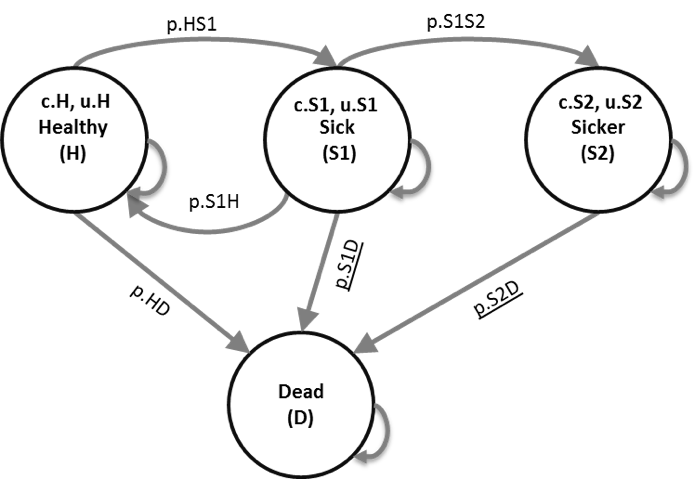
\includegraphics{../figs/Sick-Sicker figure.png}
\caption{State-transition diagram of the Sick-Sicker model. Healthy
individuals can get Sick, die or stay healthy. Sick individuals can
recover, transitioning back to healthy, can die, or stay sick. Once
individuals are Sicker, they stay Sicker until they die.
\label{fig:STM Sick-Sicker}}
\end{figure}

Two alternative strategies exist for this hypothetical disease: a
no-treatment and a treatment strategy. Under the treatment strategy,
Sick and Sicker individuals receive treatment and continue doing so
until they recover or die. The cost of the treatment is additional to
the cost of being Sick or Sicker for one year. The treatment improves
QoL for those individuals who are Sick but has no effect on the QoL of
those who are sicker. To evaluate these two alternative strategies, we
perform a CEA.

We assume that most of the parameters of the Sick-Sicker model and their
uncertainty have been previously estimated and are known to the analyst.
However, while we can identify those who are afflicted with the illness
through obvious symptoms, we can not easily distinguish those in the
Sick state from the those in the Sicker state. Thus, we can not directly
estimate state-specific mortality hazard rate ratios, nor do we know the
transition probability of progressing from Sick to Sicker. Therefore, we
calibrate the model to different epidemiological data. We internally
validated the calibrated model by comparing the predicted outputs from
the model evaluated at the calibrated parameters against the calibration
targets (Eddy et al. 2012, Goldhaber-Fiebert, Stout, and Goldie (2010)).

As part of the CEA, we conducted different deterministic sensitivity
analysis (SA), including one-way and two-way SA, and tornado plots. To
quantify the effect of parameter uncertainty on decision uncertainty, we
conducted a probabilistic sensitivity analysis (PSA) and reported our
uncertainty analysis results with a cost-effectiveness acceptability
curve (CEAC), cost-effectiveness acceptability frontier (CEAF) and
expected loss curves (ELC) (Alarid-Escudero et al. 2019). We also
conducted a value of information (VOI) analysis to determine whether
potential future research is needed to reduce parameter uncertainty. All
steps of the CEA will be described using the different components of the
framework.

\subsection{Set up}\label{set-up}

This report is a supplementary material meant to guide you through the
\texttt{R} code of a fully functional decision model to showcase the
framework described by the Decision Analysis in R for Technologies in
Health (DARTH) workgroup in the manuscript \emph{A need for change! A
coding framework for improving transparency in decision modeling}. The
code of this analysis can be downloaded from GitHub
(\url{https://github.com/DARTH-git/Decision-Modeling-Framework}). We
recommend downloading the case-study files as a single .zip file
containing all directories. Unzip the folder and save to your desired
directory. The framework is divided into different directories,
described in Table 1, that could be accessed from the RStudio project
\emph{Decision-Modeling-Framework.Rproj}. In this framework, you will
find multiple directories as described in Table 1 of the main
manuscript. We refer to the directory names of this framework and
scripts stored in these directories using \emph{italic} style. This
report is created with Markdown and is located in the \emph{reports}
directory of the framework. The figures for the case-study can be found
in the \emph{figs} directory, data required to conduct some of the
analyses of the different components are in the \emph{data} directory
and the \texttt{R} scripts with functions, are located in the
\emph{functions} directory. The main \texttt{R} scripts that conduct the
analyses of the different components of the framework are stored in the
\texttt{R} directory. In this document we do not show all the \texttt{R}
code we refer to. Therefore, it is important to follow along while
reading this document. To make sure you have all the required packages
needed to run all the code, first install all the required packages by
running the \emph{00\_general-setup.R} script in the \texttt{R}
directory.

\begin{Shaded}
\begin{Highlighting}[]
\KeywordTok{source}\NormalTok{(}\StringTok{"R/app0_packages-setup.R"}\NormalTok{)}
\end{Highlighting}
\end{Shaded}

\subsubsection{01 Define model inputs}\label{define-model-inputs}

As described in the main manuscript, in this component we declare all
model input variables and set their values. The \texttt{R} script
running the analysis of this component is the \emph{01\_model-inputs.R}
file in the \texttt{R} directory.

The input to inform the values is divided in three categories: external,
estimated, and calibrated. The majority of the Sick-Sicker model
parameters are informed by external data. Only three parameter values
need to be estimated using model calibration.

In this component, we start with the general setup of the model,
specifying among others the time horizon, name and number of health
states, proportion of the cohort in each of the different health states
at the start of the simulation and discount rates. The next step is to
specify the external parameters. The initial model parameter values and
\texttt{R} variable names are presented in Table \ref{tab:parameters}.

\begin{longtable}[]{@{}lcc@{}}
\caption{\label{tab:parameters} Description of the initial parameters
with their \texttt{R} name and value of the Sick-Sicker
model.}\tabularnewline
\toprule
\textbf{Parameter} & \textbf{R name} & \textbf{Value}\tabularnewline
\midrule
\endfirsthead
\toprule
\textbf{Parameter} & \textbf{R name} & \textbf{Value}\tabularnewline
\midrule
\endhead
Time horizon (\(n_t\)) & \texttt{n.t} & 75 years\tabularnewline
Names of health states (\(n\)) & \texttt{v.n} & H, S1, S2,
D\tabularnewline
Annual discount rate (costs/QALYs) & \texttt{d.c}/\texttt{d.e} &
3\%\tabularnewline
Annual transition probabilities & &\tabularnewline
- Disease onset (H to S1) & \texttt{p.HS1} & 0.15\tabularnewline
- Recovery (S1 to H) & \texttt{p.S1H} & 0.5\tabularnewline
- Disease progression (S1 to S2) in the time-homogenous model &
\texttt{p.S1S2} & 0.105\tabularnewline
Annual mortality & &\tabularnewline
- All-cause mortality (H to D) & \texttt{p.HD} &
age-specific\tabularnewline
- Hazard rate ratio of death in S1 vs H & \texttt{hr.S1} &
3\tabularnewline
- Hazard rate ratio of death in S2 vs H & \texttt{hr.S2} &
3\tabularnewline
Annual costs & &\tabularnewline
- Healthy individuals & \texttt{c.H} & \$2,000\tabularnewline
- Sick individuals in S1 & \texttt{c.S1} & \$4,000\tabularnewline
- Sick individuals in S2 & \texttt{c.S2} & \$15,000\tabularnewline
- Dead individuals & \texttt{c.D} & \$0\tabularnewline
- Additional costs of sick individuals treated in S1 or S2 &
\texttt{c.Trt} & \$12,000\tabularnewline
Utility weights & &\tabularnewline
- Healthy individuals & \texttt{u.H} & 1.00\tabularnewline
- Sick individuals in S1 & \texttt{u.S1} & 0.75\tabularnewline
- Sick individuals in S2 & \texttt{u.S2} & 0.50\tabularnewline
- Dead individuals & \texttt{u.D} & 0.00\tabularnewline
Intervention effect & &\tabularnewline
- Utility for treated individuals in S1 & \texttt{u.Trt} &
0.95\tabularnewline
\bottomrule
\end{longtable}

Age-specific background mortality for healthy individuals is represented
by the US population in 2015 and obtained from the
\href{https://www.mortality.org}{Human Mortality database}. This
information is stored in the \emph{01\_all-cause-mortality.csv} file in
the \emph{data} directory. Based on this .csv file a vector with
mortality rates by age is created using the \texttt{f.load\_mort\_data}
function in the \emph{01\_model-inputs\_functions.R} script. This
function gives us the flexibility to easily import data from other
countries or years.

\begin{Shaded}
\begin{Highlighting}[]
\KeywordTok{print.function}\NormalTok{(f.load_mort_data) }\CommentTok{# print the function}
\end{Highlighting}
\end{Shaded}

\begin{verbatim}
## function (file = "data/01_all-cause-mortality.csv") 
## {
##     df.r.mort_by_age <- read.csv(file = file)
##     v.r.mort_by_age <- df.r.mort_by_age %>% dplyr::select(Total) %>% 
##         as.matrix()
##     return(v.r.mort_by_age)
## }
\end{verbatim}

Another function in the \emph{01\_model-inputs\_functions.R} script, is
the \texttt{f.load\_all\_parms} function. This function, which is
actually using the \texttt{f.load\_mort\_data} function, loads all
parameters for the decision model from multiple sources and creates a
list that contains all parameters and their values.

\begin{Shaded}
\begin{Highlighting}[]
\KeywordTok{print.function}\NormalTok{(f.load_all_params)  }\CommentTok{# print the function}
\end{Highlighting}
\end{Shaded}

\begin{verbatim}
## function (file.init = "data/01_init-params.csv", file.mort = "data/01_all-cause-mortality.csv") 
## {
##     df.params.init <- read.csv(file = file.init)
##     v.r.mort_by_age <- f.load_mort_data(file = file.mort)
##     l.params.all <- with(as.list(df.params.init), {
##         v.age.names <- n.age.init:(n.age.init + n.t - 1)
##         v.n <- c("H", "S1", "S2", "D")
##         n.states <- length(v.n)
##         v.s.init <- c(H = 1, S1 = 0, S2 = 0, D = 0)
##         l.params.all <- list(n.age.init = n.age.init, n.t = n.t, 
##             v.age.names = v.age.names, v.n = v.n, n.states = n.states, 
##             v.s.init = c(H = 1, S1 = 0, S2 = 0, D = 0), v.r.mort_by_age = v.r.mort_by_age)
##         return(l.params.all)
##     })
##     l.params.all <- c(l.params.all, df.params.init)
## }
## <bytecode: 0x7fa0766ce748>
\end{verbatim}

The \texttt{f.load\_all\_params} function is informed by the arguments
\texttt{file.init} and \texttt{file.mort}. The \texttt{file.init}
argument is a string with the location and name of the file with initial
set of parameters. The initial parameter values for our case-study are
stored in the \emph{01\_init-params.csv} file located in the \emph{data}
directory. The \texttt{f.load\_all\_params} function read this .csv file
into the function environment as a dataframe called,
\texttt{df.params.init}.

The \texttt{file.mort} argument is a string with the location and name
of the file with mortality data. As described before, in our case-study
this is the \emph{01\_all-cause-mortality.csv} file. Within the
\texttt{f.load\_all\_parms} function, the \texttt{f.load\_mort\_data}
function is used to create a vector with mortality rates from the .csv
data.

After loading all the information, the \texttt{f.load\_all\_params}
generates a list called,\texttt{l.params.all}, including all parameters
for the model including the general setup parameters and the vector of
mortality rates. The function also stores the dataframe
\texttt{df.params.init} with the initial set of parameters in the list.
This is all executed in the in the \emph{01\_model-inputs.R} script by
running the code below.

\begin{Shaded}
\begin{Highlighting}[]
\NormalTok{l.params.all <-}\StringTok{ }\KeywordTok{f.load_all_params}\NormalTok{(}\DataTypeTok{file.init =} \StringTok{"data/01_init-params.csv"}\NormalTok{,}
                                  \DataTypeTok{file.mort =} \StringTok{"data/01_all-cause-mortality.csv"}\NormalTok{)}
\end{Highlighting}
\end{Shaded}

For the Sick-Sicker model we do not have to estimated parameters, but we
do have three parameters that need to be estimated via model
calibration. In this stage of the framework, we simply set these
parameters to valid ``dummy'' values that are compatible with the next
phase of the analysis, model implementation, but are ultimately just
placeholder values until we conduct the calibration phase. This means
that these values will be replaced by the best-fitted calibrated values
after we performed the calibration in component 3.

Using a function to create a list of base-case parameters to have all
model parameters in a single object is very useful, because this object
will have to be updated for the calibration and the different
sensitivity analyses in components 3 and 5 of the framework,
respectively. Below, we guide you through the components of the
function.

\subsubsection{02 Model implementation}\label{model-implementation}

In this component, we build the backbone of the decision analysis: the
implementation of the model. This component is performed by the
\emph{02\_simulation-model.R} script. This file itself is not very
large. It simply loads some packages, sources the input from component
01, sources the function \texttt{f.decision\_model} that is used the
capture the dynamic process of the Sick-Sicker example, runs this
function and stores the output. The output of the model is the
traditional cohort trace, describing how the cohort is distributed among
the different health states over time, which is plotted at the end of
this script. This trace will be used in many of the other components.

The function \texttt{f.decision\_model} is defined in the
\emph{02\_simulation-model\_functions.R file}. As described in the
paper, constructing a model as a function at this stage facilitates
subsequent stages of the model development and analysis, as these
processes will all call the same model function, but pass different
parameter values and/or calculate different final outcomes based on the
model outputs. In the next part, we will describe the code within the
function.

\begin{Shaded}
\begin{Highlighting}[]
\KeywordTok{print.function}\NormalTok{(f.decision_model) }\CommentTok{# print the code of the function}
\end{Highlighting}
\end{Shaded}

\begin{verbatim}
## function (l.params.all, verbose = FALSE) 
## {
##     with(as.list(l.params.all), {
##         p.HDage <- 1 - exp(-v.r.mort_by_age[(n.age.init + 1) + 
##             0:(n.t - 1)])
##         p.S1Dage <- 1 - exp(-v.r.mort_by_age[(n.age.init + 1) + 
##             0:(n.t - 1)] * hr.S1)
##         p.S2Dage <- 1 - exp(-v.r.mort_by_age[(n.age.init + 1) + 
##             0:(n.t - 1)] * hr.S2)
##         a.P <- array(0, dim = c(n.states, n.states, n.t), dimnames = list(v.n, 
##             v.n, 0:(n.t - 1)))
##         a.P["H", "H", ] <- (1 - p.HDage) * (1 - p.HS1)
##         a.P["H", "S1", ] <- (1 - p.HDage) * p.HS1
##         a.P["H", "D", ] <- p.HDage
##         a.P["S1", "H", ] <- (1 - p.S1Dage) * p.S1H
##         a.P["S1", "S1", ] <- (1 - p.S1Dage) * (1 - (p.S1S2 + 
##             p.S1H))
##         a.P["S1", "S2", ] <- (1 - p.S1Dage) * p.S1S2
##         a.P["S1", "D", ] <- p.S1Dage
##         a.P["S2", "S2", ] <- 1 - p.S2Dage
##         a.P["S2", "D", ] <- p.S2Dage
##         a.P["D", "D", ] <- 1
##         m.indices.notvalid <- arrayInd(which(a.P < 0 | a.P > 
##             1), dim(a.P))
##         try(if (dim(m.indices.notvalid)[1] != 0) {
##             v.rows.notval <- rownames(a.P)[m.indices.notvalid[, 
##                 1]]
##             v.cols.notval <- colnames(a.P)[m.indices.notvalid[, 
##                 2]]
##             v.cycles.notval <- dimnames(a.P)[[3]][m.indices.notvalid[, 
##                 3]]
##             df.notvalid <- data.frame(`Transition probabilities not valid:` = matrix(paste0(paste(v.rows.notval, 
##                 v.cols.notval, sep = "->"), "; at cycle ", v.cycles.notval), 
##                 ncol = 1), check.names = FALSE)
##             if (verbose) {
##                 message("Not valid transition probabilities")
##                 stop(print(df.notvalid), call. = FALSE)
##             }
##         })
##         valid <- apply(a.P, 3, function(x) all.equal(sum(rowSums(x)), 
##             n.states))
##         if (!isTRUE(all.equal(as.numeric(sum(valid)), as.numeric(n.t)))) {
##             if (verbose) {
##                 stop("This is not a valid transition Matrix")
##             }
##         }
##         m.M <- matrix(0, nrow = (n.t + 1), ncol = n.states, dimnames = list(0:n.t, 
##             v.n))
##         m.M[1, ] <- v.s.init
##         for (t in 1:n.t) {
##             m.M[t + 1, ] <- m.M[t, ] %*% a.P[, , t]
##         }
##         return(list(a.P = a.P, m.M = m.M))
##     })
## }
## <bytecode: 0x7fa0793befa8>
\end{verbatim}

The \texttt{f.decision\_model} function is informed by the argument
\texttt{l.params.all}. Via this argument we give the function a list
with all parameters of the decision model. For the Sick-Sicker model,
these parameters are stored in the list \texttt{l.params.all}, which we
passed into the function as shown below.

\begin{Shaded}
\begin{Highlighting}[]
\NormalTok{l.out.stm <-}\StringTok{ }\KeywordTok{f.decision_model}\NormalTok{(}\DataTypeTok{l.params.all =}\NormalTok{ l.params.all) }\CommentTok{# run the function}
\end{Highlighting}
\end{Shaded}

This function itself has all the mathematical equations of the decision
models coded inside. It starts by calculating the age-specific
transition probabilities from all non-dead states based on the vector of
age-specific mortality rates \texttt{v.r.asr}. These parameters will
become vectors of length \texttt{n.t}, describing the probability to die
for all ages from all non-dead states.

The next part of the function, creates an array that stores the
age-specific transition probability matrices in each of the third
dimension. The transition probability matrix is a core component of a
state-transition cohort model (Iskandar 2018). This matrix contains the
probabilities of transitioning from the current health state, indicated
by the rows, to the other health states, specified by the columns. Since
we have age-specific transition probabilities, the transition
probability matrix is different at each cycle. These probabilities are
only depending on the age of the cohort, and not on other events;
therefore, we can generate all matrices at the start of the model. This
results in \texttt{n.t} different age-specific matrices that are stored
in an array, called \texttt{a.P}, of dimensions \texttt{n.s} x
\texttt{n.s} x \texttt{n.t}. After initializing the array, it is filled
with the transition probability stored in the list. When running the
model, we can index the correct transition probability matrix
corresponding with the current age of the cohort. We then added some
sanity checks to make sure that the transition matrices and the
transition probabilities are valid. The transition probability matrices
stored in the array \texttt{a.P}, for the first three and last cycle,
are shown below.

\begin{Shaded}
\begin{Highlighting}[]
\NormalTok{l.out.stm}\OperatorTok{$}\NormalTok{a.P[, , }\DecValTok{1}\OperatorTok{:}\DecValTok{3}\NormalTok{] }\CommentTok{# show the first three time-points of a.P}
\end{Highlighting}
\end{Shaded}

\begin{verbatim}
## , , 0
## 
##            H        S1        S2           D
## H  0.8491385 0.1498480 0.0000000 0.001013486
## S1 0.4984813 0.3938002 0.1046811 0.003037378
## S2 0.0000000 0.0000000 0.9899112 0.010088764
## D  0.0000000 0.0000000 0.0000000 1.000000000
## 
## , , 1
## 
##            H        S1        S2            D
## H  0.8491513 0.1498502 0.0000000 0.0009985012
## S1 0.4985037 0.3938180 0.1046858 0.0029925135
## S2 0.0000000 0.0000000 0.9900597 0.0099402657
## D  0.0000000 0.0000000 0.0000000 1.0000000000
## 
## , , 2
## 
##            H        S1        S2           D
## H  0.8490910 0.1498396 0.0000000 0.001069428
## S1 0.4983976 0.3937341 0.1046635 0.003204853
## S2 0.0000000 0.0000000 0.9893570 0.010642959
## D  0.0000000 0.0000000 0.0000000 1.000000000
\end{verbatim}

\begin{Shaded}
\begin{Highlighting}[]
\NormalTok{l.out.stm}\OperatorTok{$}\NormalTok{a.P[, , l.params.all}\OperatorTok{$}\NormalTok{n.t] }\CommentTok{# show it for the last cycle}
\end{Highlighting}
\end{Shaded}

\begin{verbatim}
##            H        S1         S2         D
## H  0.6055199 0.1068564 0.00000000 0.2876237
## S1 0.1807584 0.1427991 0.03795926 0.6384833
## S2 0.0000000 0.0000000 0.03365849 0.9663415
## D  0.0000000 0.0000000 0.00000000 1.0000000
\end{verbatim}

By comparing these probability matrices, we observe an increase in the
probabilities of transitioning to death from all health states.

After the array is filled, the cohort trace matrix, \texttt{m.M}, of
dimensions \texttt{n.t} x \texttt{n.s} is initialized. This matrix will
store the state occupation at each point in time. The first row of the
matrix is informed by the initial state vector \texttt{v.s.init}. For
the remaining points in time, we iteratively multiply the cohort trace
with the age-specific transition probability matrix corresponding to the
specific cycle obtained by indexing the array \texttt{a.P}
appropriately. All the outputs and relevant elements of the decision
model are stored in a list, called \texttt{l.out.stm}. This list
contains the array of the transition probability matrix for all cycles
\texttt{t} and the cohort trace \texttt{m.M}.

\begin{Shaded}
\begin{Highlighting}[]
\KeywordTok{head}\NormalTok{(l.out.stm}\OperatorTok{$}\NormalTok{m.M)    }\CommentTok{# show the top part of the cohort trace}
\end{Highlighting}
\end{Shaded}

\begin{verbatim}
##           H        S1         S2           D
## 0 1.0000000 0.0000000 0.00000000 0.000000000
## 1 0.8491385 0.1498480 0.00000000 0.001013486
## 2 0.7957468 0.1862564 0.01568695 0.002309774
## 3 0.7684912 0.1925699 0.03501425 0.003924648
## 4 0.7484793 0.1909659 0.05478971 0.005765035
## 5 0.7306193 0.1873106 0.07413838 0.007931783
\end{verbatim}

\begin{Shaded}
\begin{Highlighting}[]
\KeywordTok{tail}\NormalTok{(l.out.stm}\OperatorTok{$}\NormalTok{m.M)    }\CommentTok{# show the bottom part of the cohort trace}
\end{Highlighting}
\end{Shaded}

\begin{verbatim}
##              H           S1           S2         D
## 70 0.009928317 0.0022433565 2.035951e-04 0.9876247
## 71 0.007153415 0.0015935925 1.311619e-04 0.9911218
## 72 0.005058845 0.0011174473 8.674540e-05 0.9937370
## 73 0.003460336 0.0007552206 5.436484e-05 0.9957301
## 74 0.002289594 0.0004937081 3.298632e-05 0.9971837
## 75 0.001475636 0.0003151589 1.985106e-05 0.9981894
\end{verbatim}

Using the code below, we can graphically show the model dynamics by
plotting the cohort trace. Figure \ref{fig:Sick-Sicker-Trace} shows the
distribution of the cohort among the different health states at each
time point.

\begin{figure}
\centering
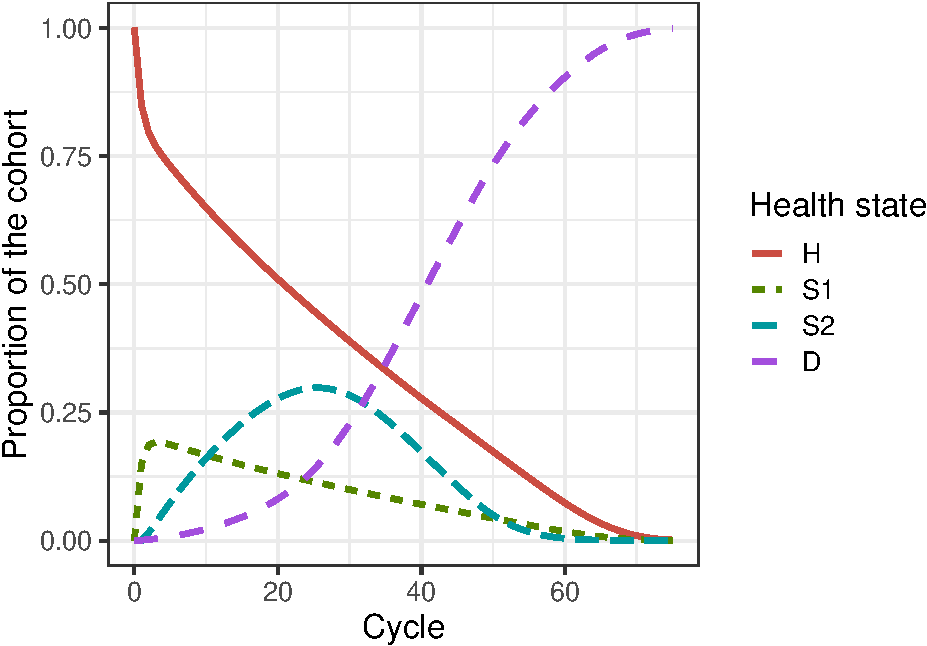
\includegraphics{Case_study_Sick-Sicker_Framework_files/figure-latex/Sick-Sicker-Trace-1.pdf}
\caption{Cohort trace of the Sick-Sicker cohort
model\label{fig:Sick-Sicker-Trace}}
\end{figure}

\subsubsection{03 Model calibration}\label{model-calibration}

In this component, we calibrate unknown model parameters by matching
model outputs to specified calibration targets. Specifically, we
calibrate the Sick-Sicker model to match survival, prevalence and the
proportion who are Sicker, among all those afflicted (Sick+Sicker). We
used a Bayesian calibration approach using the incremental mixture
importance sampling (IMIS) algorithm (Steele, Raftery, and Emond 2006),
which has been used to calibrate health policy models (Raftery and Bao
2010, Menzies et al. (2017), Rutter et al. (2018)). Bayesian methods
allow us to quantify the uncertainty in the calibrated parameters even
in the presence of non-identifiability (Alarid-Escudero et al. 2018).
This analysis is coded in the \emph{03\_calibration.R} file. The target
data is stored in the \emph{03\_calibration-targets.RData} file. Similar
to component 02, in the section \emph{03.1 Load packages}, data and
functions we start by loading inputs and functions. In addition, we load
the calibration targets data into the R workspace. In the next section,
\emph{03.2 Visualize targets}, we plot each of the calibration targets
with their confidence intervals.

In section \emph{03.3 Run calibration algorithms}, we set the parameters
we like to calibrate to fixed values and test if the function
\texttt{f.calibration\_out} that produces model outputs corresponding to
the calibration targets works. This function takes a vector of
parameters that need to be calibrated and a list with all parameters of
decision model and computes model outputs to be used for calibration
routines.

\begin{Shaded}
\begin{Highlighting}[]
\KeywordTok{print.function}\NormalTok{(f.calibration_out) }\CommentTok{# print the functions}
\end{Highlighting}
\end{Shaded}

\begin{verbatim}
## function (v.params.calib, l.params.all) 
## {
##     l.params.all <- f.update_param_list(l.params.all = l.params.all, 
##         params.updated = v.params.calib)
##     l.out.stm <- f.decision_model(l.params.all = l.params.all)
##     v.os <- 1 - l.out.stm$m.M[, "D"]
##     v.prev <- rowSums(l.out.stm$m.M[, c("S1", "S2")])/v.os
##     v.prop.S2 <- l.out.stm$m.M[, "S2"]/rowSums(l.out.stm$m.M[, 
##         c("S1", "S2")])
##     l.out <- list(Surv = v.os[c(11, 21, 31)], Prev = v.prev[c(11, 
##         21, 31)], PropSicker = v.prop.S2[c(11, 21, 31)])
##     return(l.out)
## }
\end{verbatim}

This function is informed by two argument \texttt{v.params.calib} and
\texttt{l.params.all}. The vector \texttt{v.params.calib} contains the
values of the three parameters of interest and the list
\texttt{l.params.all} contains all parameters of the decision model. The
placeholder values are replaced by \texttt{v.params.calib} and with
these values the model is evaluated. This is done by running the
\texttt{f.decision\_model} function, described in component 02. This
results in a new list with output of the model corresponding to the
parameter values in the \texttt{v.params.calib}. With this new decision
model output, the overall survival, disease prevalence and the
proportion of Sicker in the Sick and Sicker states are calculated. The
estimated values for these epidemiological outcomes at different
timepoints are combined in a list called \texttt{l.out} produced but the
\texttt{f.calibration\_out}.

Once we make sure this code works, we specify the calibration parameters
in section \emph{03.3.1 Specify calibration parameters}. These include
setting the seed for the random number generation, specifying the number
of random samples to obtain from the calibrated posterior distribution,
the name of the input parameters and the range of these parameters that
will inform the prior distributions of the calibrated parameters, and
the name of the calibration targets: \texttt{Surv}, \texttt{Prev},
\texttt{PropSick}.

In the next section, \emph{03.3.2 Run IMIS algorithm}, we calibrate the
Sick-Sicker model with the IMIS algorithm. For this case-study, we
assume a normal likelihood and uniform priors but other could be used.
For a more detailed description of IMIS for Bayesian calibration,
different likelihood functions and prior distributions, we refer the
reader to the tutorial for Bayesian calibration by Menzies et al.
(Menzies et al. 2017). We use the \texttt{IMIS} function from the
\texttt{IMIS} package that calls the functions \texttt{likelihood},
\texttt{sample.prior} and \texttt{prior}, to draw samples from the
posterior distribution (A. Raftery and Le Bao 2012). The functions are
specified in the \emph{03\_calibration\_functions.R} file. For the
\texttt{IMIS} function, we specify the incremental sample size at each
iteration of IMIS, the desired posterior sample size at the resample
stage, the maximum number of iterations in IMIS and the number of
optimizers which could be 0. The function returns a list, which we call
\texttt{l.fit.imis}, with the posterior samples, the diagnostic
statistics at each IMIS iteration and the centers of Gaussian components
(A. Raftery and Le Bao 2012). We store the posterior samples in the
matrix \texttt{m.calib.post}.

We then explore these posterior distributions in section \emph{03.4
Exploring posterior distribution}. We start by estimating the posterior
mean, median and 95\% credible interval, the mode and the
maximum-a-posteriori (MAP). To estimate the mode, we use the package
\texttt{modeest} (Poncet 2018). All for these summary statistics are
combined in a dataframe called \texttt{df.posterior.summ}. Table
\ref{tab:SummaryCal} shows the summary statistics of the posterior
distribution.

\begin{table}[t]

\caption{\label{tab:unnamed-chunk-11}Summary statistics of the posterior distribution\label{tab:SummaryCal}}
\centering
\begin{tabular}{l|r|r|r|r|r|r}
\hline
  & Mean & 2.5\% & 50\% & 97.5\% & Mode & MAP\\
\hline
p.S1S2 & 0.1077822 & 0.0966154 & 0.107619 & 0.1206907 & 0.1071694 & 0.1078278\\
\hline
hr.S1 & 2.7151807 & 1.1007592 & 2.608970 & 4.4139330 & 1.9654838 & 2.2970418\\
\hline
hr.S2 & 9.5435354 & 7.1631569 & 9.534398 & 11.8839979 & 9.2717728 & 9.8870386\\
\hline
\end{tabular}
\end{table}

In section \emph{03.4.2 Visualization of posterior distribution}, we
generate a pairwise scatter plot of the calibrated parameters (Figure
\ref{fig:03_posterior-distribution-marginal}) and a 3D scatter plot of
the joint posterior distribution (Figure
\ref{fig:Posterior-distribution-joint}). These figures are saved in the
\emph{figs} directory.

\begin{figure}
\centering
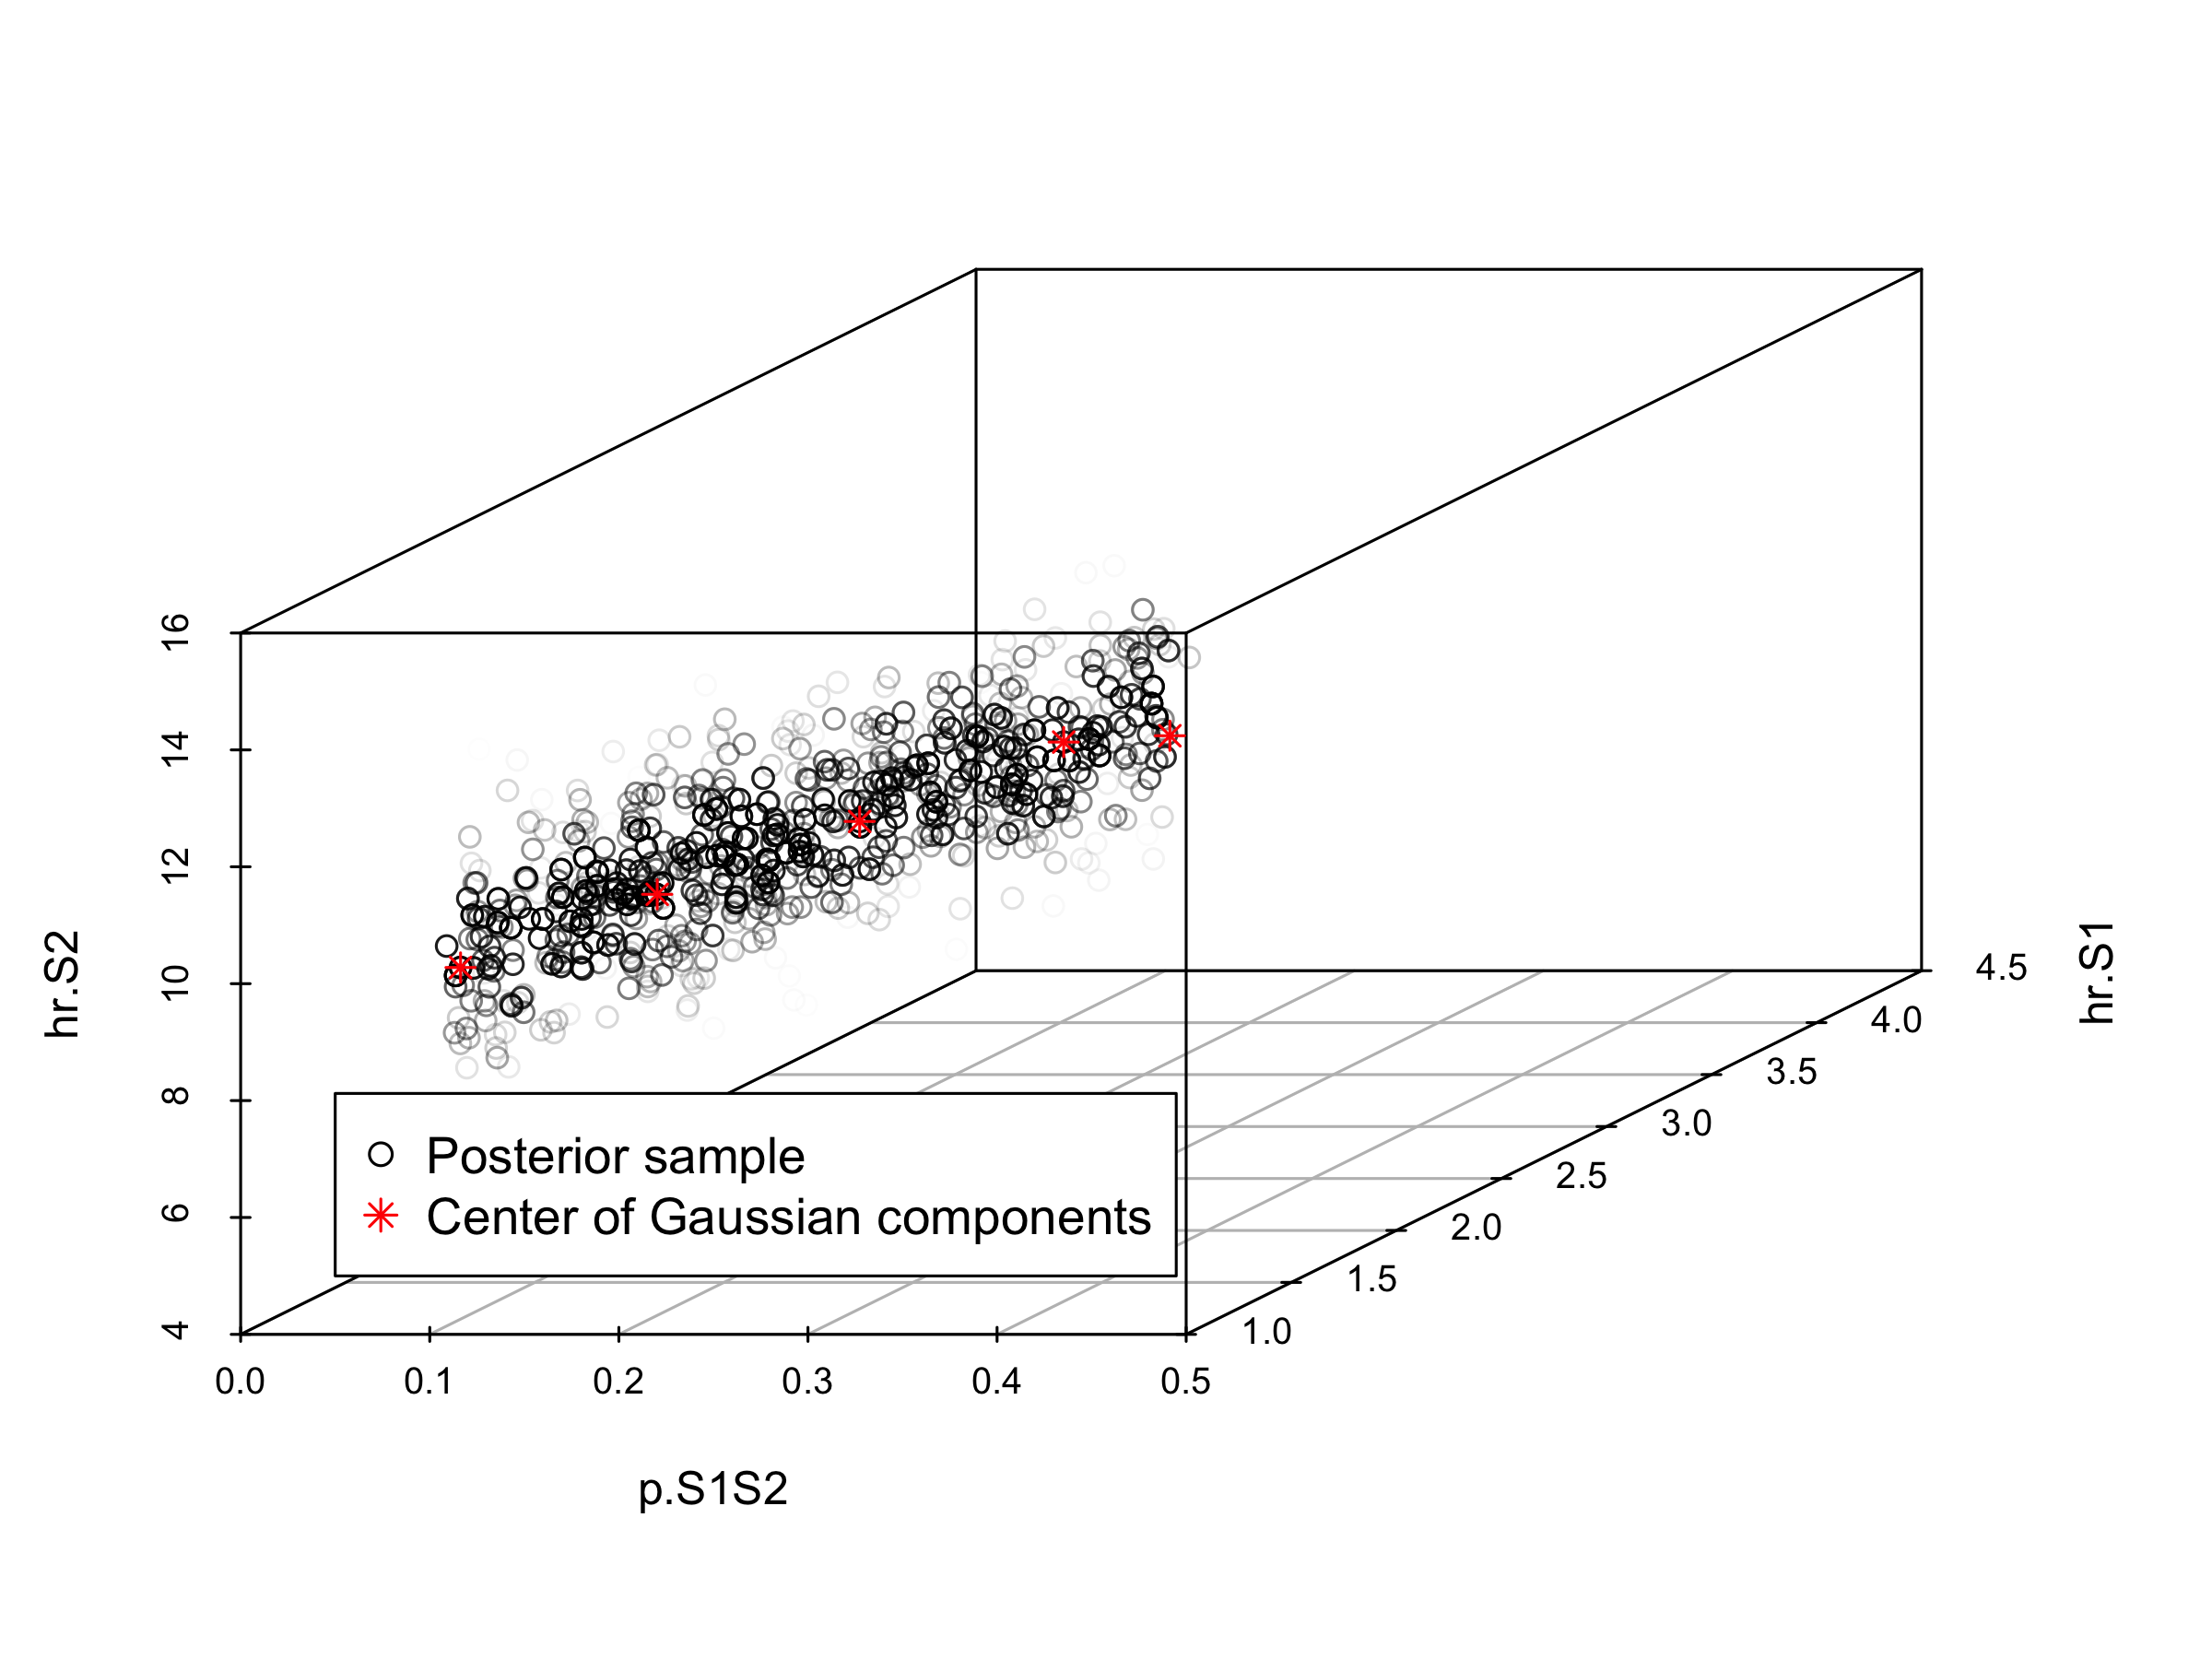
\includegraphics{../figs/03_posterior-distribution-joint.png}
\caption{Joint posterior distribution
\label{fig:Posterior-distribution-joint}}
\end{figure}

\begin{figure}
\centering
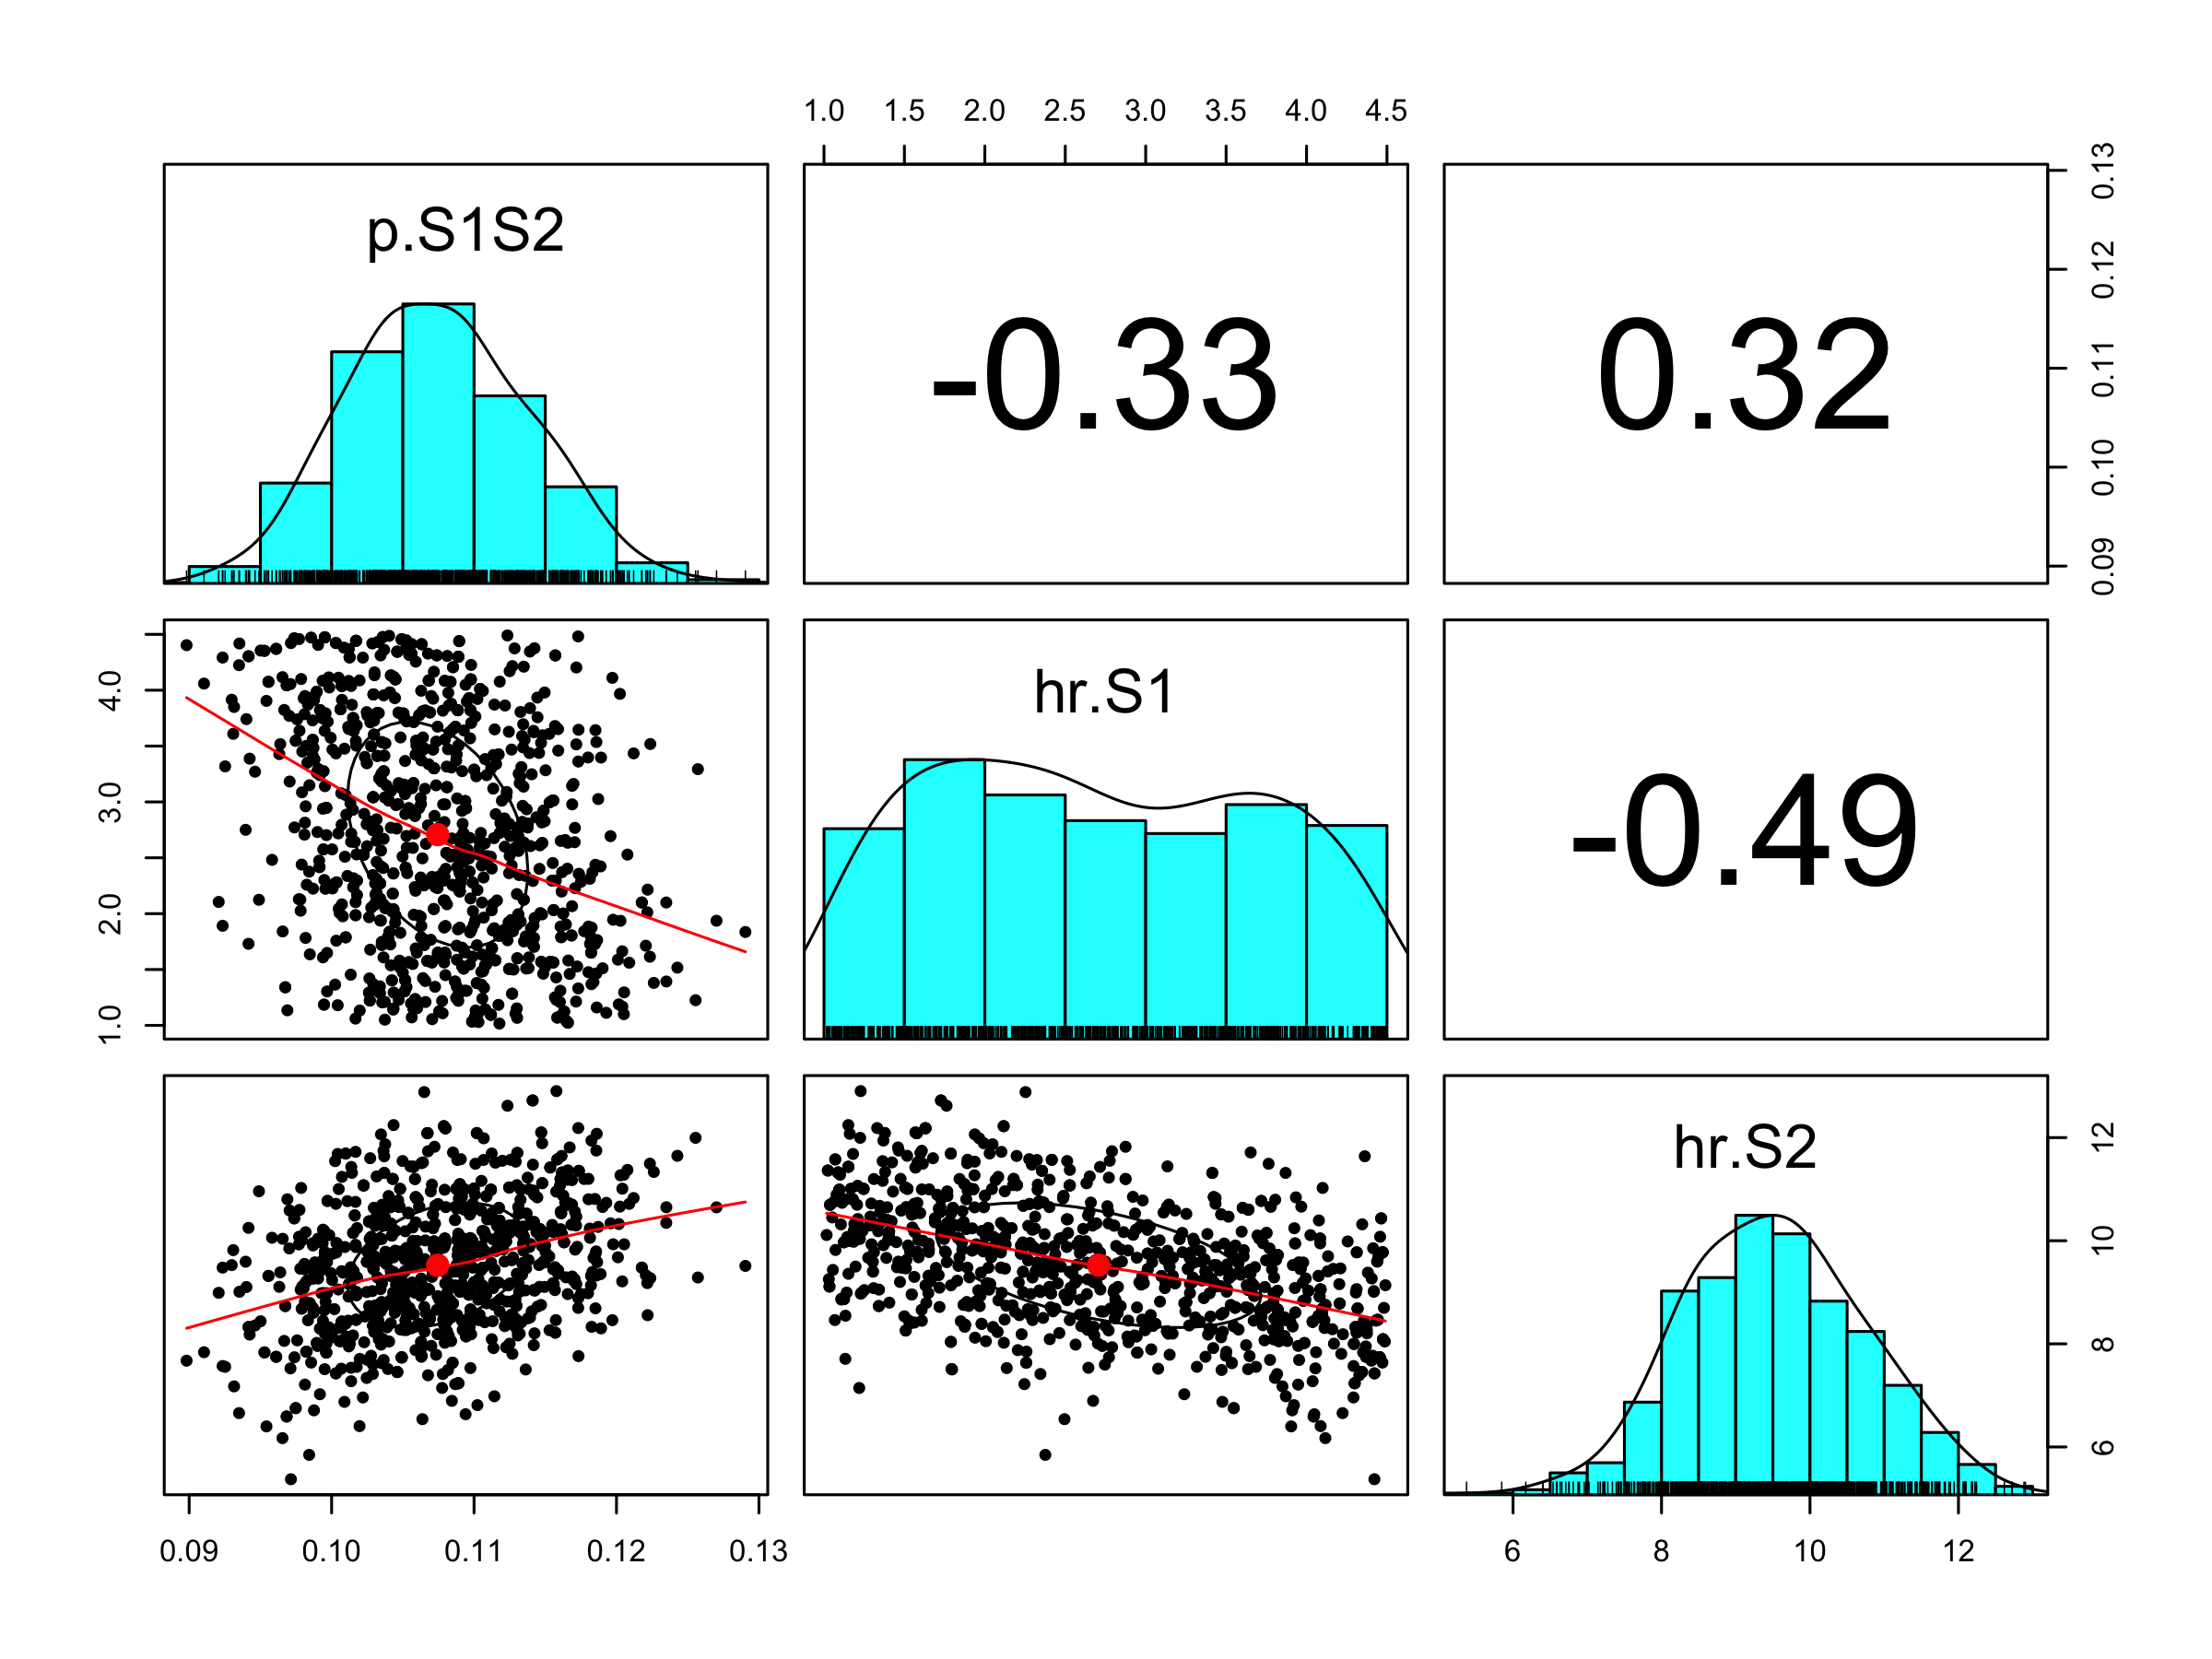
\includegraphics{../figs/03_posterior-distribution-marginal.png}
\caption{Pairwise posterior distribution of calibrated parameters
\label{fig:03_posterior-distribution-marginal}}
\end{figure}

Finally, the posterior distribution and MAP estimate from the IMIS
calibration are stored in the file \emph{03\_imis-output.RData}. Storing
this data as an .Rdata file allows to import the data in following
sections without needing to re-run the calibration component.

\subsubsection{04 Validation}\label{validation}

In this section, we check the internal validity of our Sick-Sicker model
before we move on to the analysis components. To internally validate the
Sick-Sicker model, we compare the model-predicted output evaluated at
posterior parameters against the calibration targets. This is all done
in the \emph{04\_validation.R} script by loading all previously
described functions and the generated calibration targets.

In section \emph{04.2 Compute model-predicted outputs}, we compute the
model-predicted outputs for each sample of posterior distribution as
well as for the MAP estimate. We then use the function
\texttt{f.data\_summary} to summarize the model-predicted posterior
outputs into different summary statistics.

\begin{Shaded}
\begin{Highlighting}[]
\KeywordTok{print.function}\NormalTok{(f.data_summary)}
\end{Highlighting}
\end{Shaded}

\begin{verbatim}
## function (data, varname, groupnames) 
## {
##     require(plyr)
##     summary_func <- function(x, col) {
##         c(mean = mean(x[[col]], na.rm = TRUE), median = quantile(x[[col]], 
##             probs = 0.5, names = FALSE), sd = sd(x[[col]], na.rm = TRUE), 
##             lb = quantile(x[[col]], probs = 0.025, names = FALSE), 
##             ub = quantile(x[[col]], probs = 0.975, names = FALSE))
##     }
##     data_sum <- ddply(data, groupnames, .fun = summary_func, 
##         varname)
##     data_sum <- plyr::rename(data_sum, c(mean = varname))
##     return(data_sum)
## }
## <bytecode: 0x7fa075c4b468>
\end{verbatim}

This function is informed by three arguments, \texttt{data},
\texttt{varname} and \texttt{groupnames}.

The computation of the model-predicted outputs using the MAP estimate is
done by inserting the \texttt{v.calib.post.map} data into the previously
described \texttt{f.calibration\_out} function. This function creates a
list including the estimated values for survival, prevalence and the
proportion of sicker individuals at cycles 10, 20 and 30.

In sections \emph{04.6 Internal validation: Model-predicted outputs
vs.~targets}, we check the internal validation by plotting the
model-predicted outputs against the calibration targets (Figure
\ref{fig:04_surv}-\ref{fig:04_proportion}). The generated plots are
saved as .png files, which could be used in reports later on without the
need of re-running the code.

\begin{figure}
\centering
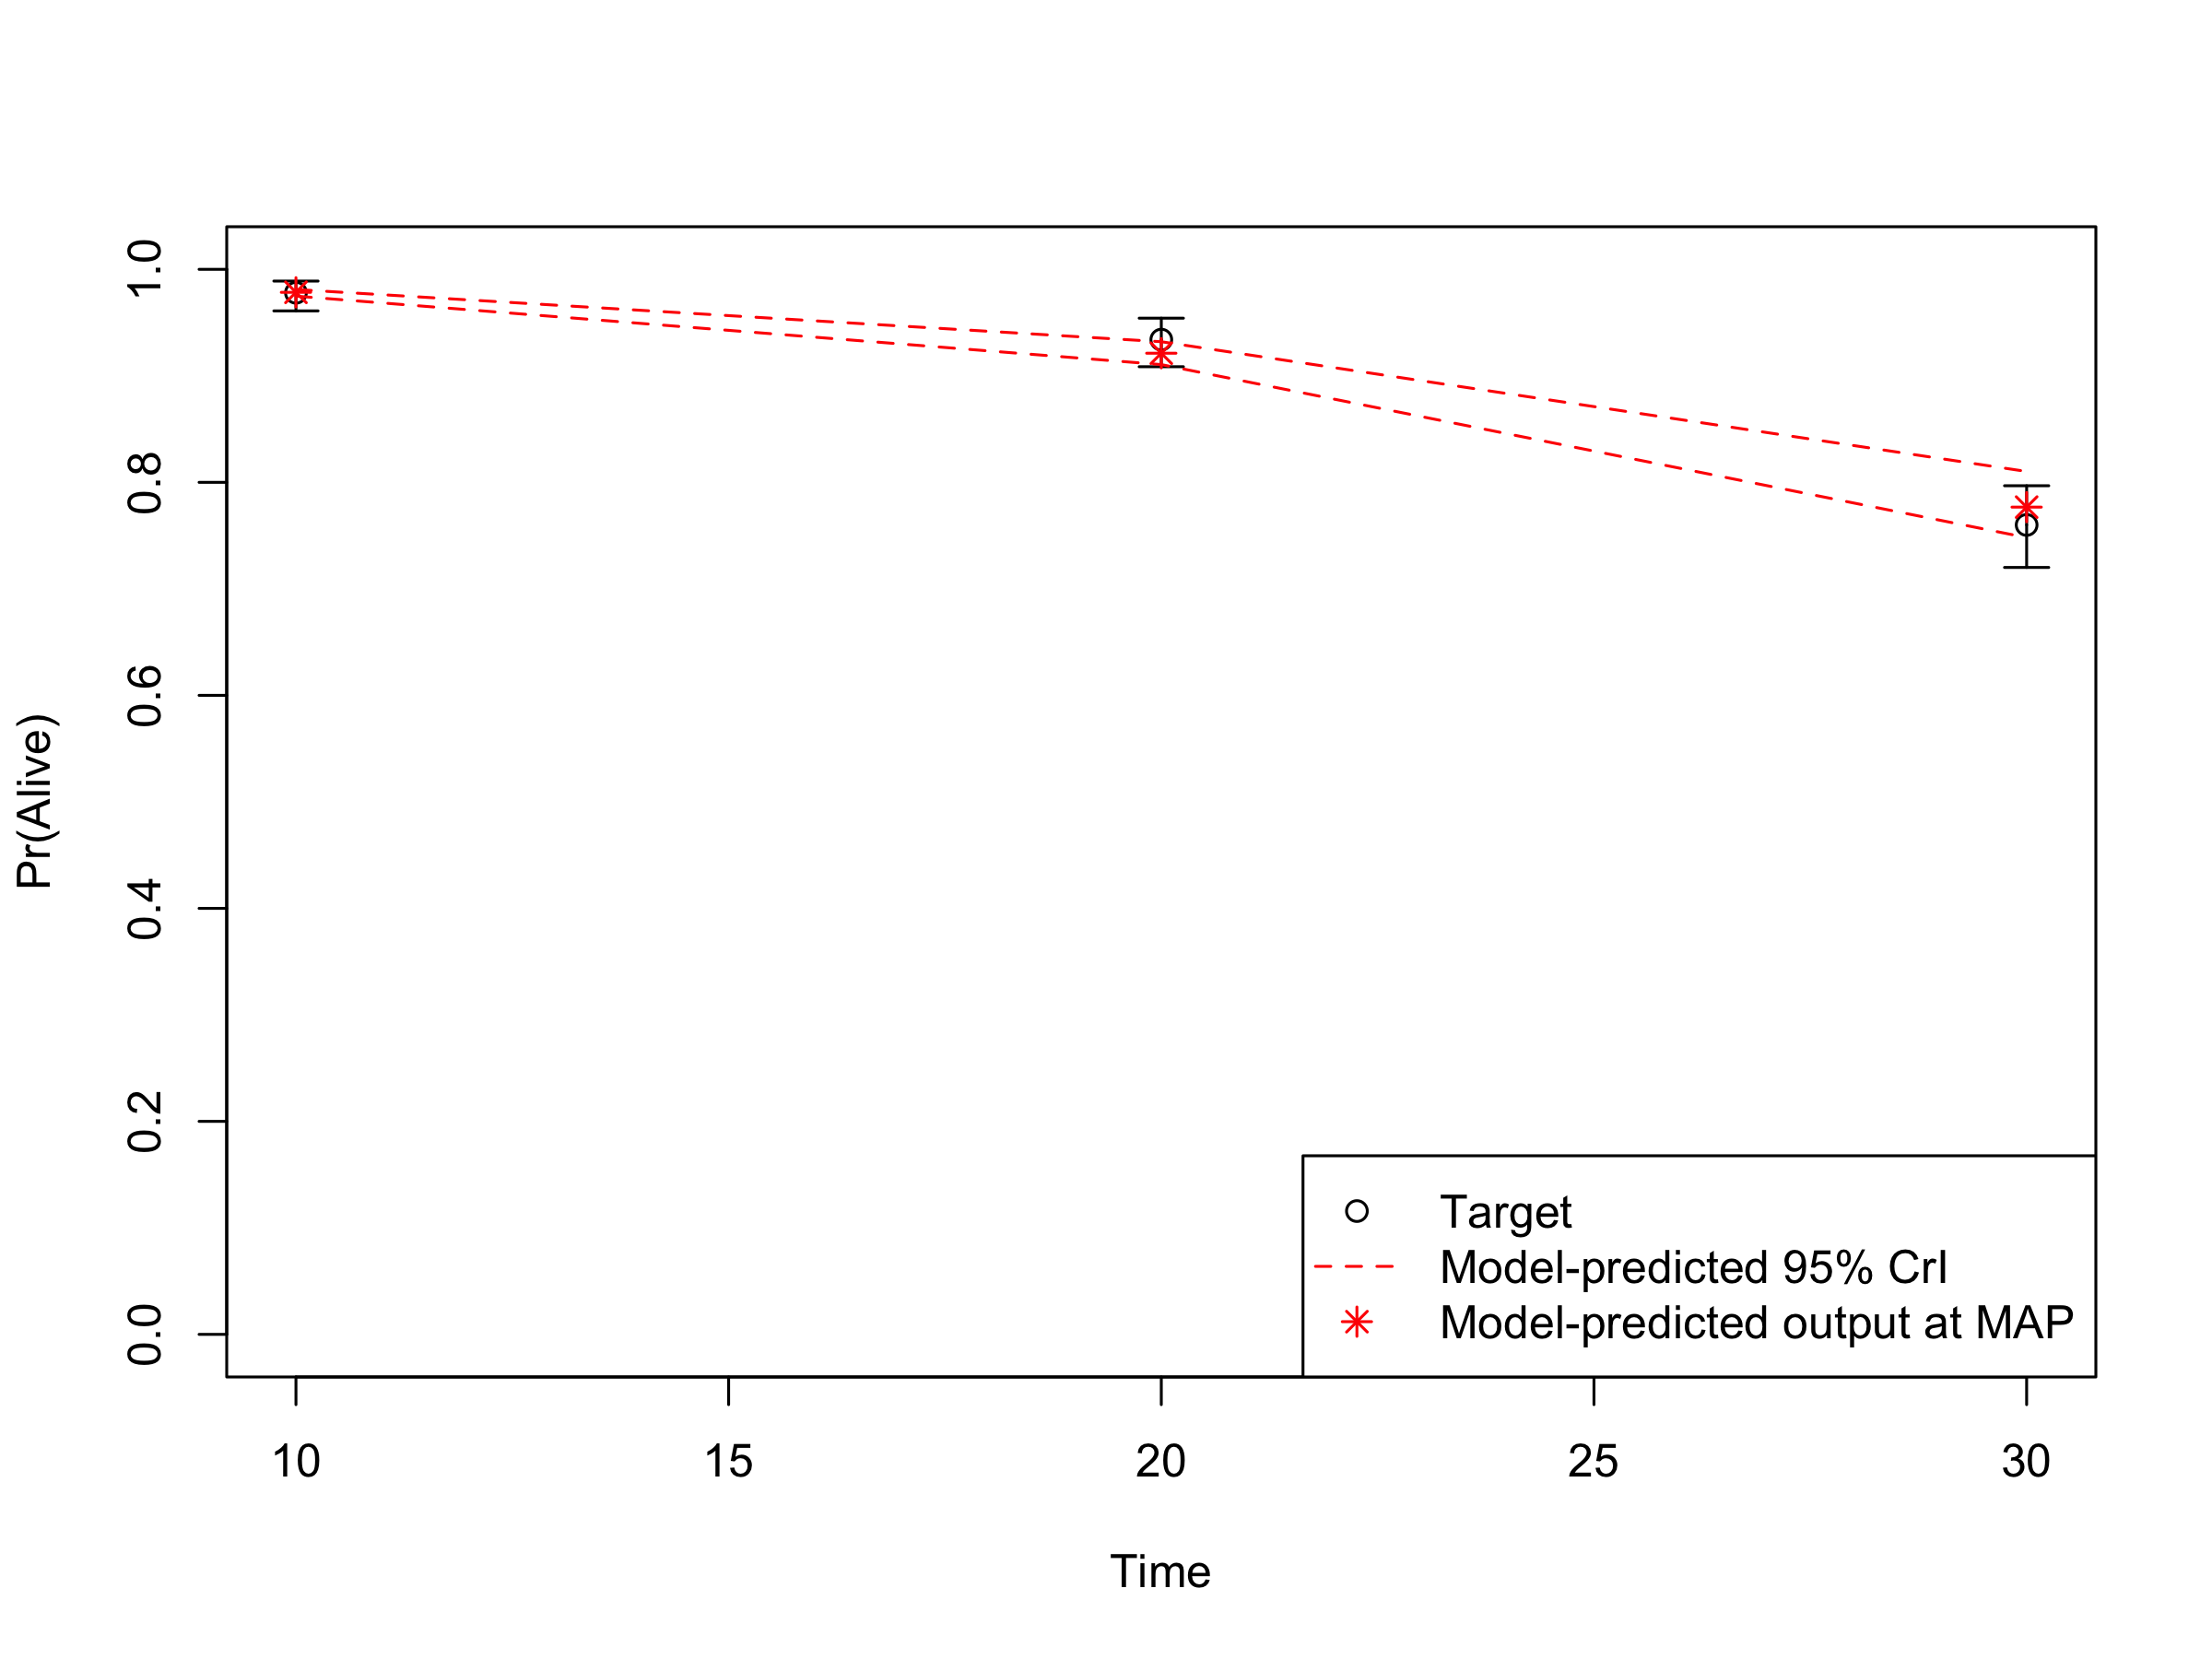
\includegraphics{../figs/04_posterior-vs-targets-survival.png}
\caption{Survival data: Model-predicted outputs vs targets
\label{fig:04_surv}}
\end{figure}

\begin{figure}
\centering
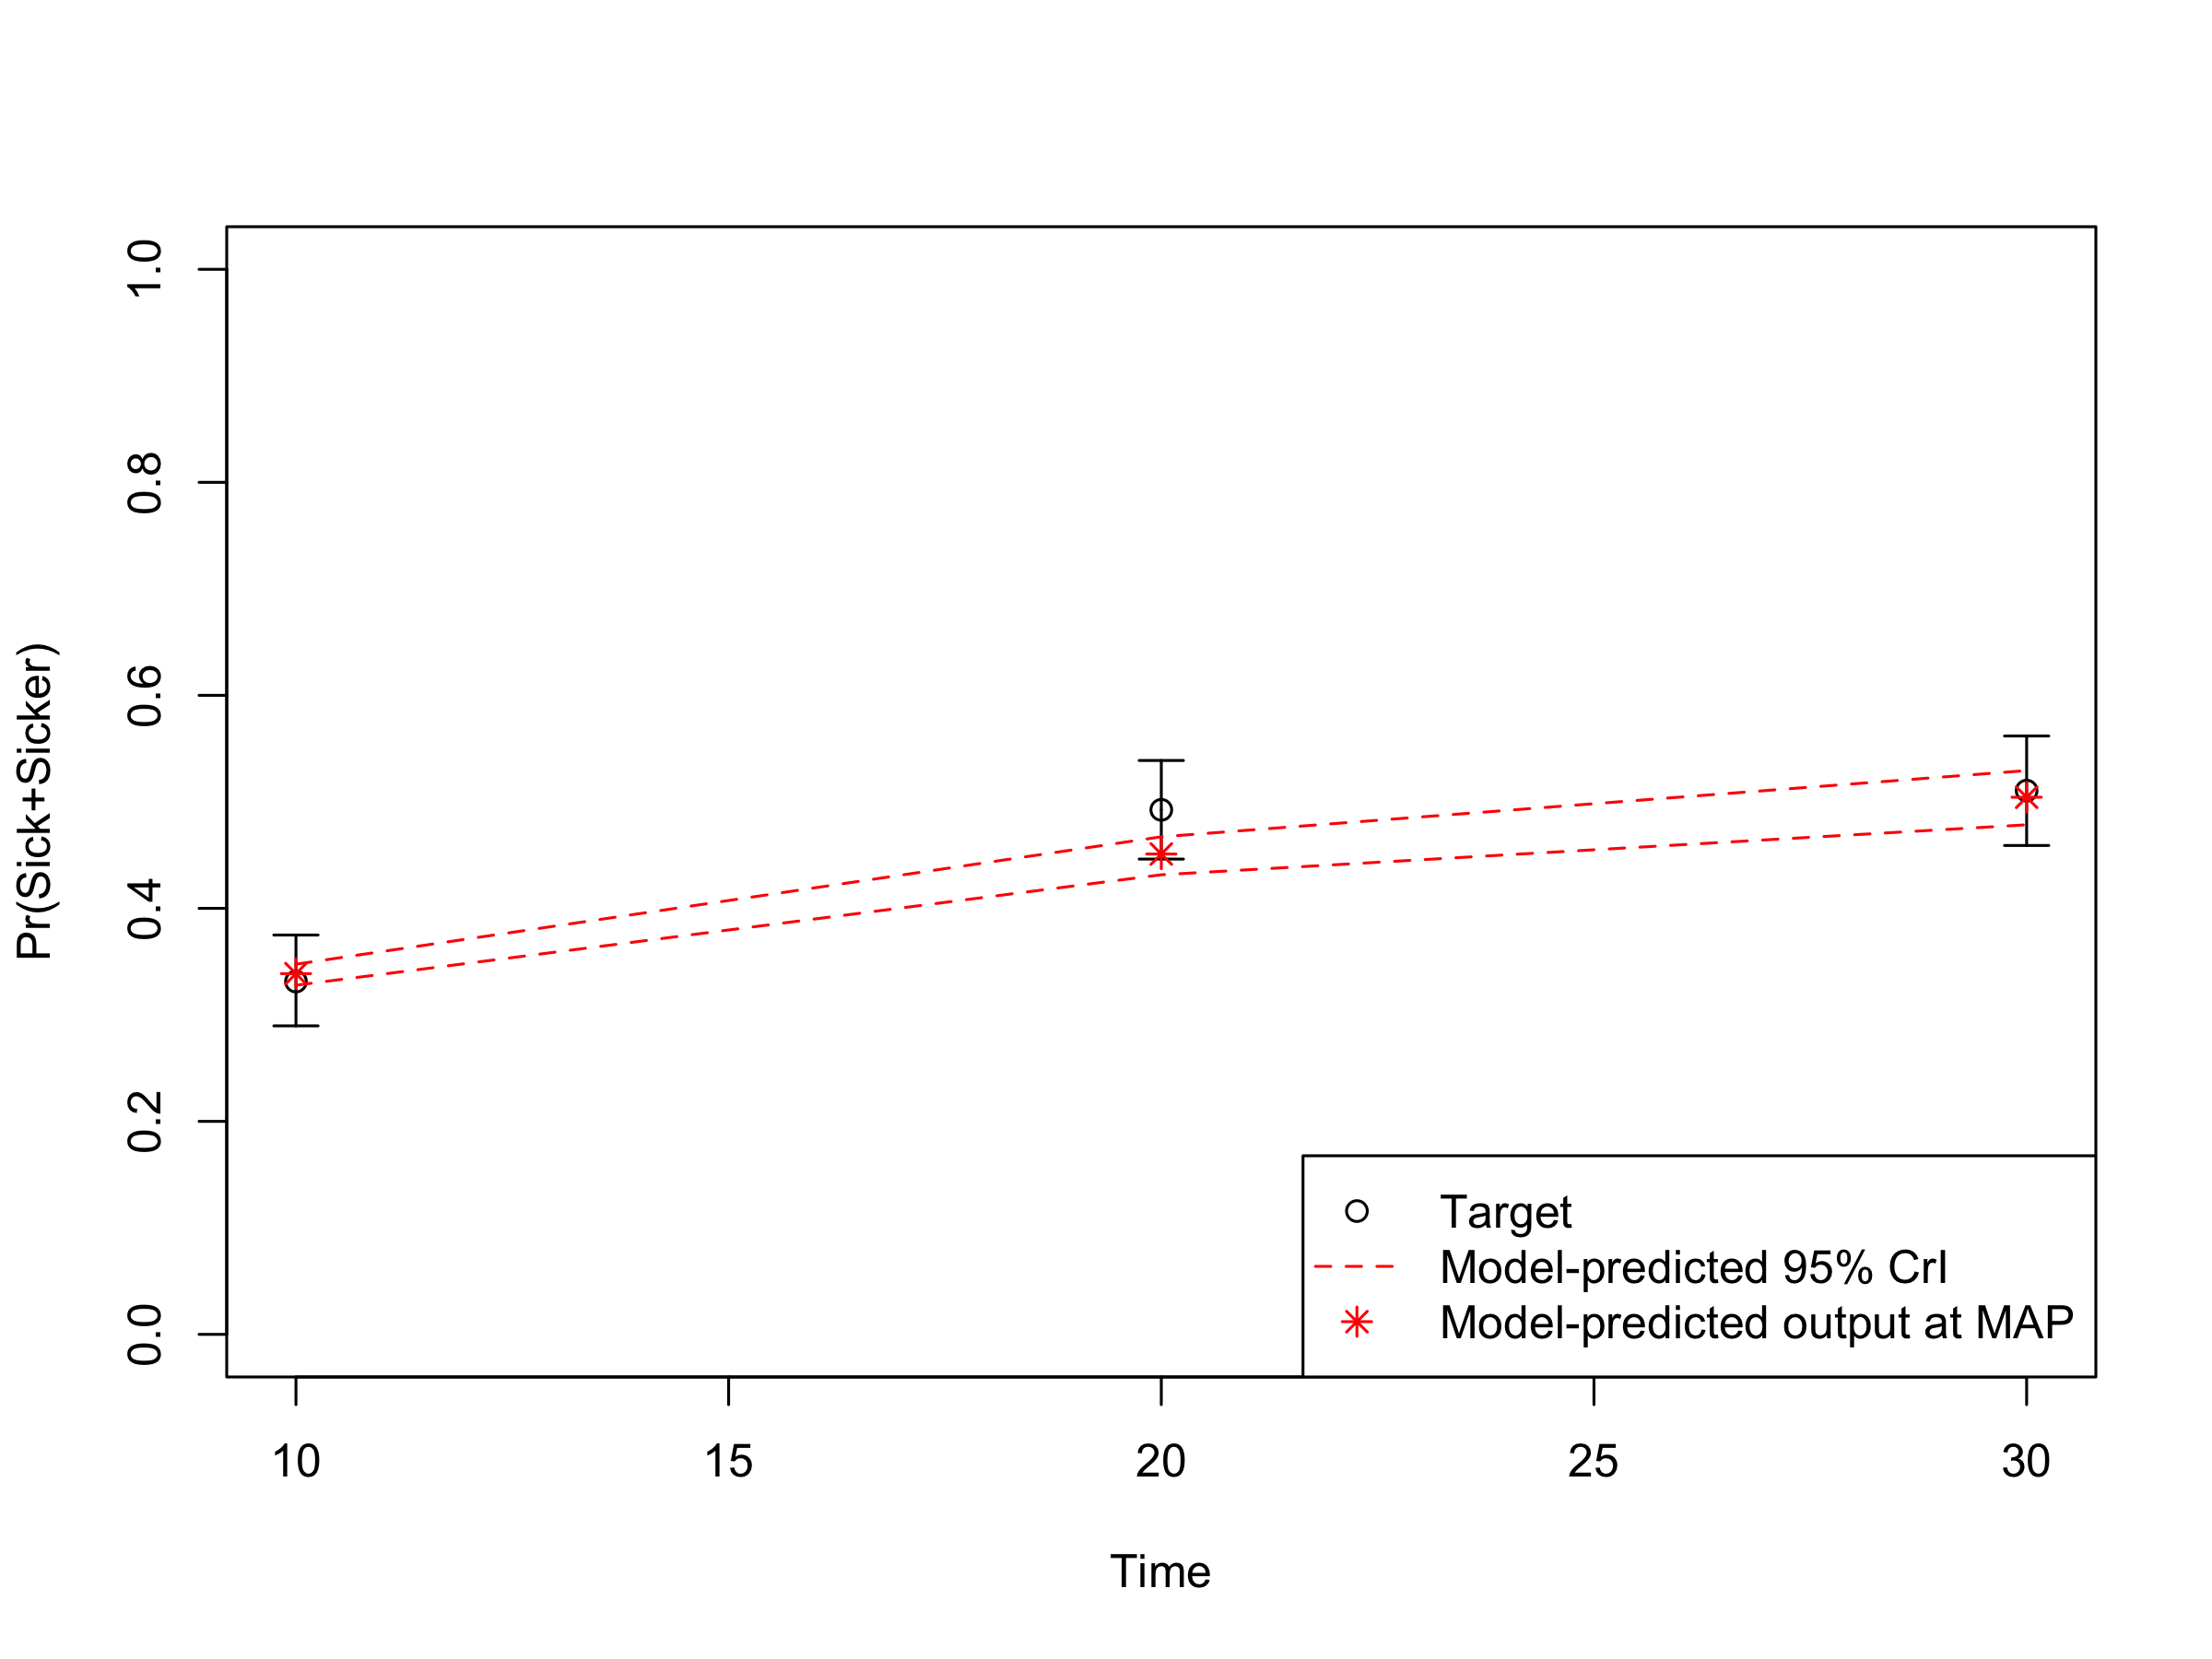
\includegraphics{../figs/04_posterior-vs-targets-prevalence.png}
\caption{Prevalence data of sick individuals: Model-predicted output vs
targets \label{fig:04_p}}
\end{figure}

\begin{figure}
\centering
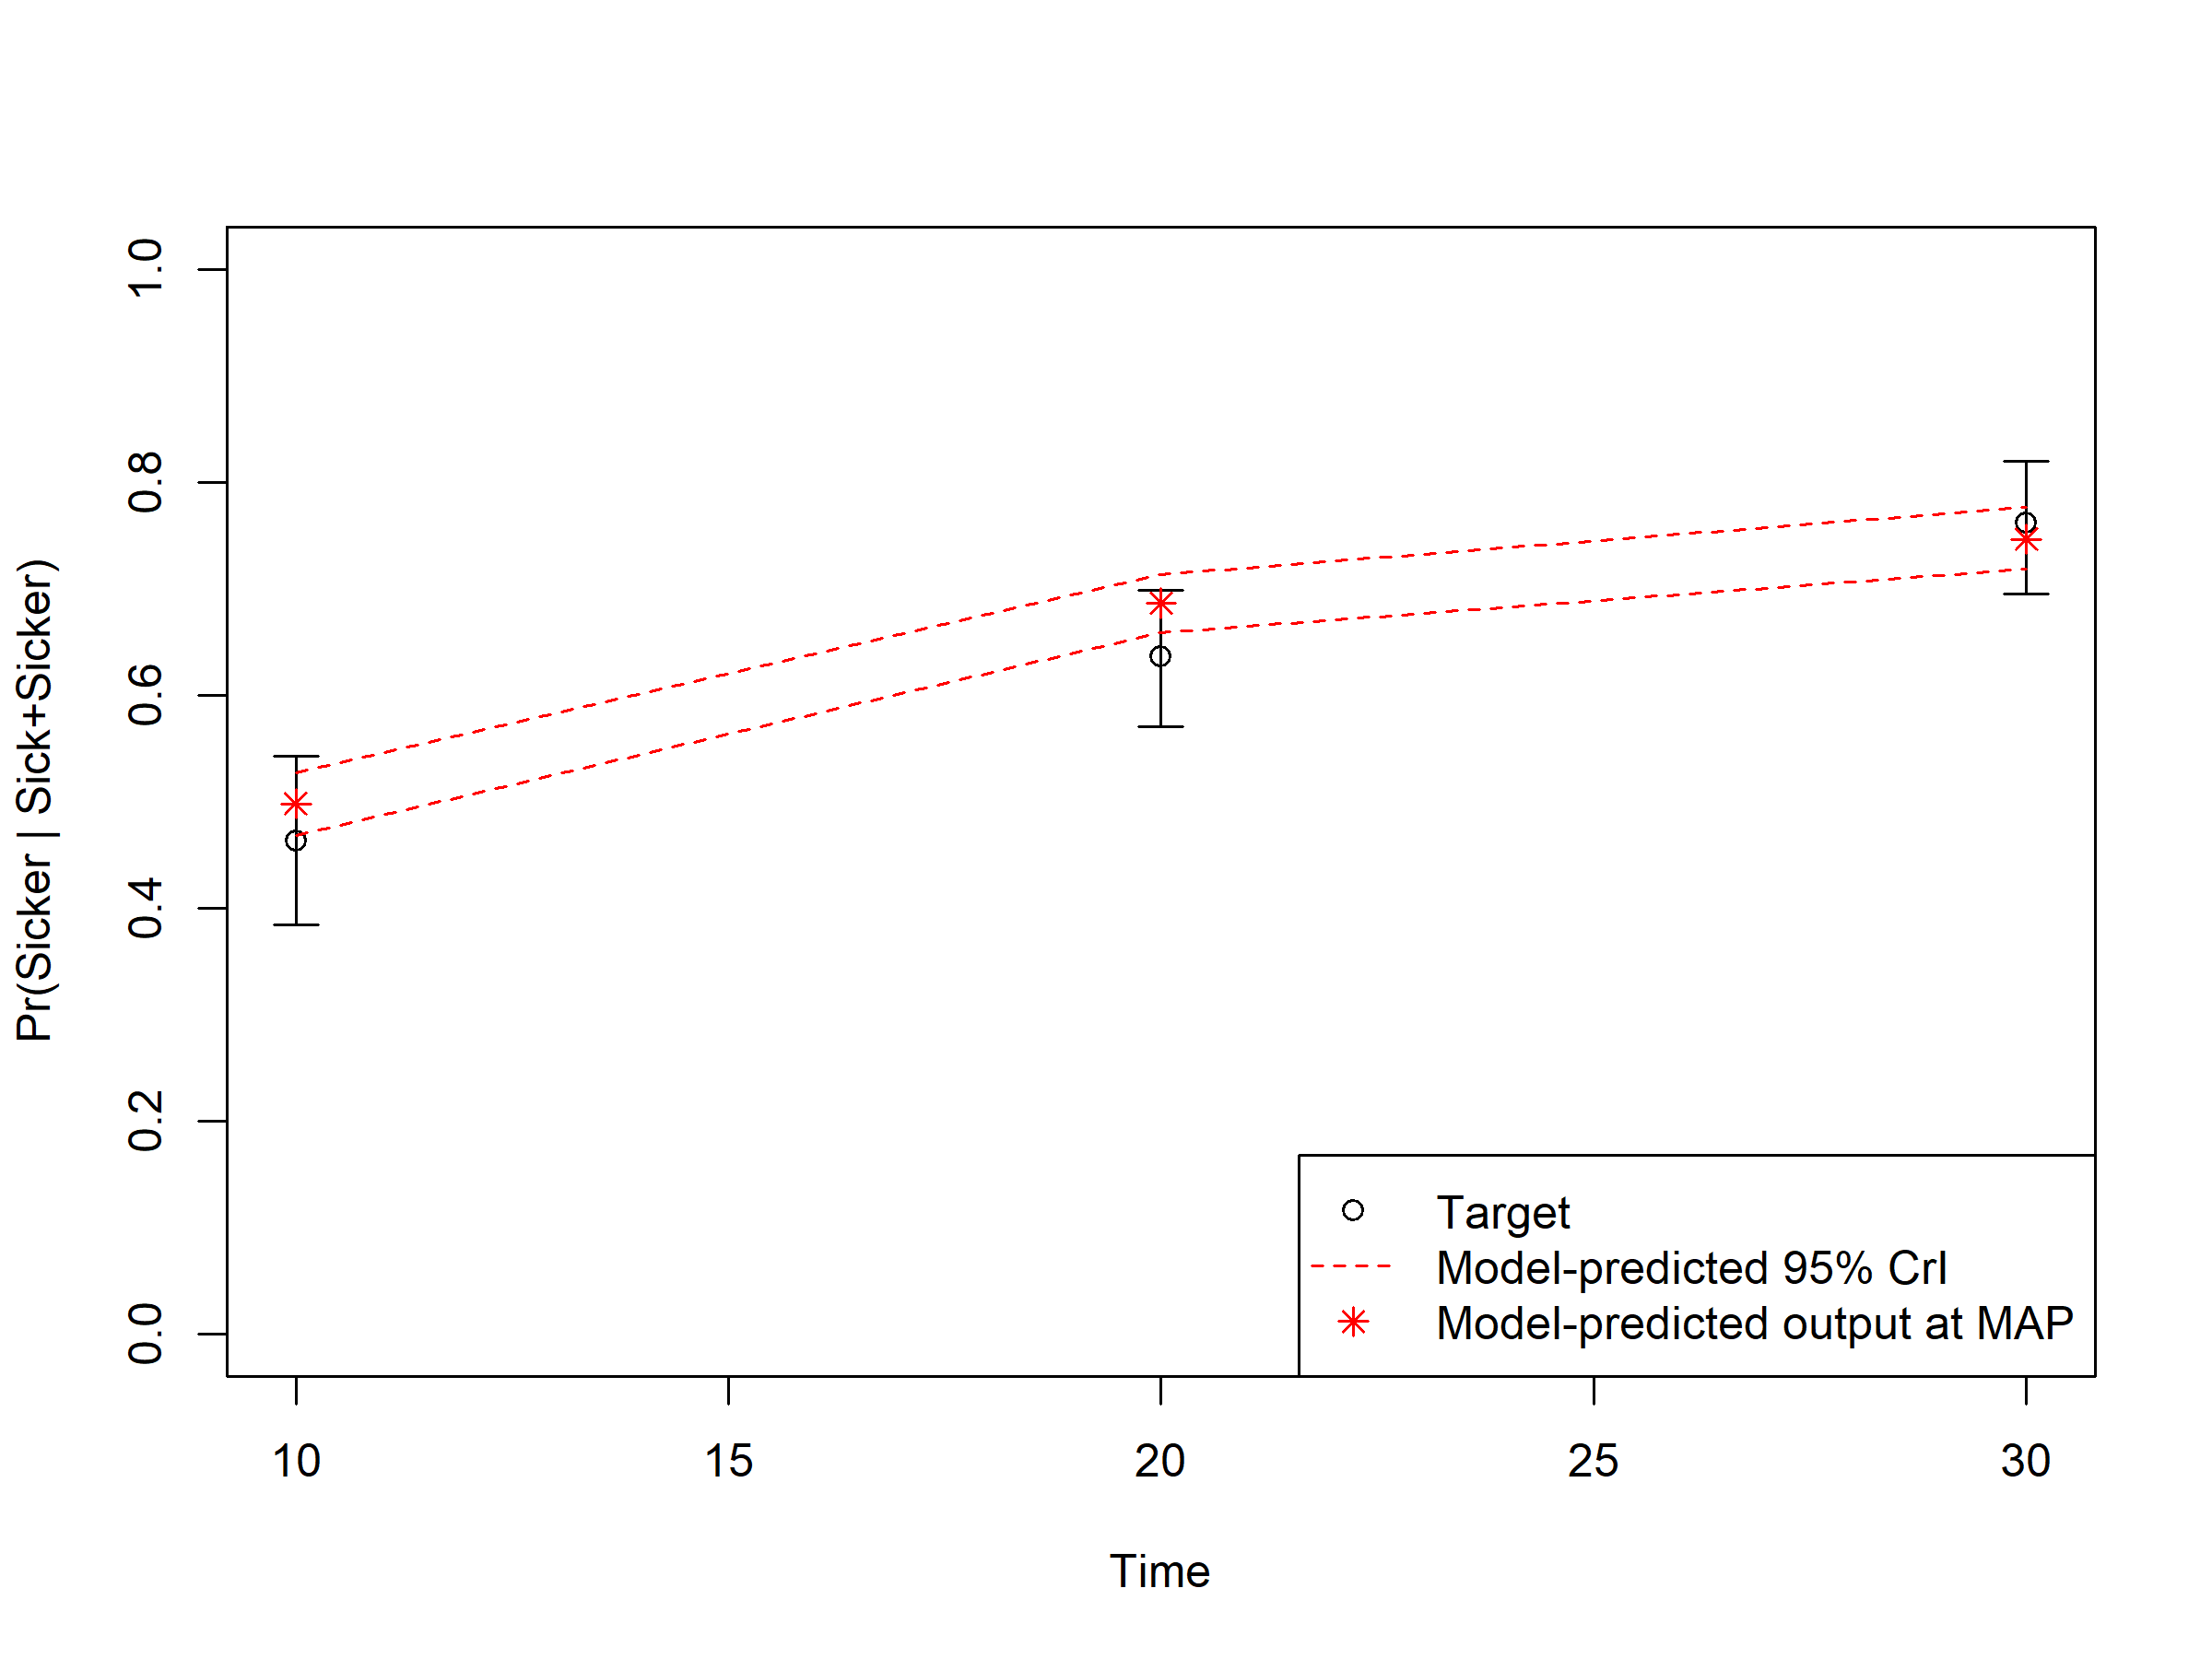
\includegraphics{../figs/04_posterior-vs-targets-proportion-sicker.png}
\caption{Proportion who are Sicker, among all those afflicted (Sick +
Sicker): Model-predicted output \label{fig:04_proportion}}
\end{figure}

\subsubsection{05: Analysis}\label{analysis}

The analysis component is where the elements in components 1-4 are
combined to answer the question(s) of interest given current information
and to quantify the value of potential further research. Our framework
separates the analysis in three subcomponents: \emph{05a Deterministic
analysis}, \emph{05b Uncertainty analysis} and \emph{05c Value of
information analysis}. For the Sick-Sicker case-study, we use all three
subcomponents to conduct the CEA and to quantify the uncertainty of our
decision. For procedures in the CEA, we rely on the \texttt{R} package
\texttt{dampack}, which is available here:
\url{https://github.com/DARTH-git/dampack}. Instructions for installing
\texttt{dampack} are described in Appendix 0 provided in the
\emph{app0\_packages-setup.R} script.

\paragraph{05a Deterministic analysis}\label{a-deterministic-analysis}

In this subcomponent, we perform a deterministic CEA, followed by some
deterministic sensitivity analysis, including one-way, two-way and
tornado sensitivity analyses. The function script of this subcomponent,
\emph{05a\_deterministic-analysis\_function.R}, contains the function
\texttt{f.calculate\_ce\_out}. This function calculates costs and
effects for a given vector of parameters using a simulation model. We
need to run our simulation model using the calibrated parameter values,
but the list we created in component 01 still contain the placeholder
values for the calibrated parameters. This means we need to update these
values by the calibrated values stored in the vector
\texttt{v.calib.post.map}. The \emph{00\_general\_functions.R} script in
the \emph{functions} folder creates the \texttt{f.update\_param\_list}
function that is able to update a list of parameters with new values for
some specific parameters.

\begin{Shaded}
\begin{Highlighting}[]
\KeywordTok{print.function}\NormalTok{(f.update_param_list)}
\end{Highlighting}
\end{Shaded}

\begin{verbatim}
## function (l.params.all, params.updated) 
## {
##     if (typeof(params.updated) != "list") {
##         params.updated <- split(unname(params.updated), names(params.updated))
##     }
##     l.params.all <- modifyList(l.params.all, params.updated)
##     return(l.params.all)
## }
## <bytecode: 0x7fa07670eb38>
\end{verbatim}

The first argument of the function, called \texttt{l.params.all}, is a
list with all the parameters of decision model. The second argument,
\texttt{params.updated}, is an object with parameters for which values
need to be updated. The function returns the list \texttt{l.params.all}
with updated values.

In the \emph{05a\_deterministic-analysis.R} script we execute the
\texttt{f.update\_param\_list} function for our case-study, resulting in
the list \texttt{l.params.basecase} where the placeholder values for
\texttt{p.S1S2}, \texttt{hr.S1} and \texttt{hr.S2} are replaced by the
calibration estimates.

\begin{Shaded}
\begin{Highlighting}[]
\NormalTok{l.params.basecase <-}\StringTok{ }\KeywordTok{f.update_param_list}\NormalTok{(l.params.all, v.calib.post.map) }
\end{Highlighting}
\end{Shaded}

We use this new list as an argument in the \texttt{f.calculate\_ce\_out}
function. In addition, we specify the willingness-to-pay (WTP) threshold
value using the \texttt{n.wtp} argument of this function. This WTP value
is used to compute a net monetary benefit (NMB) value. If the user does
not specify the WTP, a default value of \$100,000/QALY will be used by
the function.

\begin{Shaded}
\begin{Highlighting}[]
\NormalTok{df.out.ce <-}\StringTok{ }\KeywordTok{f.calculate_ce_out}\NormalTok{(}\DataTypeTok{l.params.all =}\NormalTok{ l.params.basecase, }
                                \DataTypeTok{n.wtp =} \DecValTok{150000}\NormalTok{)}
\KeywordTok{print.function}\NormalTok{(f.calculate_ce_out) }\CommentTok{# print the function}
\end{Highlighting}
\end{Shaded}

\begin{verbatim}
## function (l.params.all, n.wtp = 1e+05) 
## {
##     with(as.list(l.params.all), {
##         v.dwc <- 1/((1 + d.e)^(0:(n.t)))
##         v.dwe <- 1/((1 + d.c)^(0:(n.t)))
##         l.model.out.no_trt <- f.decision_model(l.params.all = l.params.all)
##         l.model.out.trt <- f.decision_model(l.params.all = l.params.all)
##         m.M_no_trt <- l.model.out.no_trt$m.M
##         m.M_trt <- l.model.out.trt$m.M
##         v.u_no_trt <- c(u.H, u.S1, u.S2, u.D)
##         v.u_trt <- c(u.H, u.Trt, u.S2, u.D)
##         v.c_no_trt <- c(c.H, c.S1, c.S2, c.D)
##         v.c_trt <- c(c.H, c.S1 + c.Trt, c.S2 + c.Trt, c.D)
##         v.tu_no_trt <- m.M_no_trt %*% v.u_no_trt
##         v.tu_trt <- m.M_trt %*% v.u_trt
##         v.tc_no_trt <- m.M_no_trt %*% v.c_no_trt
##         v.tc_trt <- m.M_trt %*% v.c_trt
##         tu.d_no_trt <- t(v.tu_no_trt) %*% v.dwe
##         tu.d_trt <- t(v.tu_trt) %*% v.dwe
##         tc.d_no_trt <- t(v.tc_no_trt) %*% v.dwc
##         tc.d_trt <- t(v.tc_trt) %*% v.dwc
##         v.tc.d <- c(tc.d_no_trt, tc.d_trt)
##         v.tu.d <- c(tu.d_no_trt, tu.d_trt)
##         v.nmb.d <- v.tu.d * n.wtp - v.tc.d
##         df.ce <- data.frame(Strategy = v.names.str, Cost = v.tc.d, 
##             Effect = v.tu.d, NMB = v.nmb.d)
##         return(df.ce)
##     })
## }
## <bytecode: 0x7fa07eb31068>
\end{verbatim}

After calculating the discount weights, this function runs the
simulation model using the previously described function
\texttt{f.decision\_model} in the
\emph{02\_simulatiomn-model\_function.R} script. Inside the function
\texttt{f.calculate\_ce\_out}, the simulation model is run for both the
treatment, \texttt{l.model.out.trt}, and no treatment,
\texttt{l.model.out.no\_trt}, strategies of the Sick-Sicker model.
Running it for both treatment strategies is done for illustration
purposes. In this case-study, the resulting cohort traces are identical
and we could have executed it only once.

In the second part of the function we create multiple vectors for both
the cost and effects of both strategies. These vectors multiply the
cohort trace to compute the cycle-specific rewards. This results in
vectors of total costs (\texttt{v.tc}) and total effects (\texttt{v.tu})
per cycle. By multiplying these vectors with the vectors with the
discount weights for costs (\texttt{v.dwc}) and effects (\texttt{v.dwe})
we get the total discounted mean costs (\texttt{tc.d\_no\_trt} and
\texttt{tc.d\_trt}) and QALYs (\texttt{tu.d\_no\_trt} and
\texttt{tu.d\_trt}) for both strategies. These values are used in the
calculation of the NMB. Finally, the total discounted costs,
effectiveness and NMB are combined in the dataframe \texttt{df.ce}. The
results for our case-study are shown below.

\begin{Shaded}
\begin{Highlighting}[]
\NormalTok{df.out.ce }\CommentTok{# print the dataframe }
\end{Highlighting}
\end{Shaded}

\begin{verbatim}
##       Strategy     Cost   Effect     NMB
## 1 No Treatment 115239.8 20.02366 2888309
## 2    Treatment 214157.6 20.72299 2894291
\end{verbatim}

This dataframe of CE results can be used as an argument in the
\texttt{calculate\_icers} function from the \texttt{dampack} package to
calculate the incremental cost-effectiveness ratios (ICERs) and noting
which strategies are weakly and strongly dominated. Table
\ref{tab:df.cea.det} shows the result of the deterministic CEA.

\begin{Shaded}
\begin{Highlighting}[]
\NormalTok{df.cea.det <-}\StringTok{ }\KeywordTok{calculate_icers}\NormalTok{(}\DataTypeTok{cost =}\NormalTok{ df.out.ce}\OperatorTok{$}\NormalTok{Cost, }
                              \DataTypeTok{effect =}\NormalTok{ df.out.ce}\OperatorTok{$}\NormalTok{Effect, }
                              \DataTypeTok{strategies =}\NormalTok{ v.names.str)}
\end{Highlighting}
\end{Shaded}

\begin{table}[t]

\caption{\label{tab:unnamed-chunk-18}Deterministic cost-effectiveness analysis results of the Sick-Sicker model comparing no treatment with treatment \label{tab:df.cea.det}}
\centering
\begin{tabular}{l|r|r|r|r|r}
\hline
Strategy & Cost & Effect & Inc\_Cost & Inc\_Effect & ICER\\
\hline
No Treatment & 115239.8 & 20.02366 & NA & NA & NA\\
\hline
Treatment & 214157.6 & 20.72299 & 98917.83 & 0.6993333 & 141445.9\\
\hline
\end{tabular}
\end{table}

Finally, Figure \ref{fig:05a_CEA-frontier} shows the cost-effectiveness
frontier of the CEA.

\begin{figure}
\centering
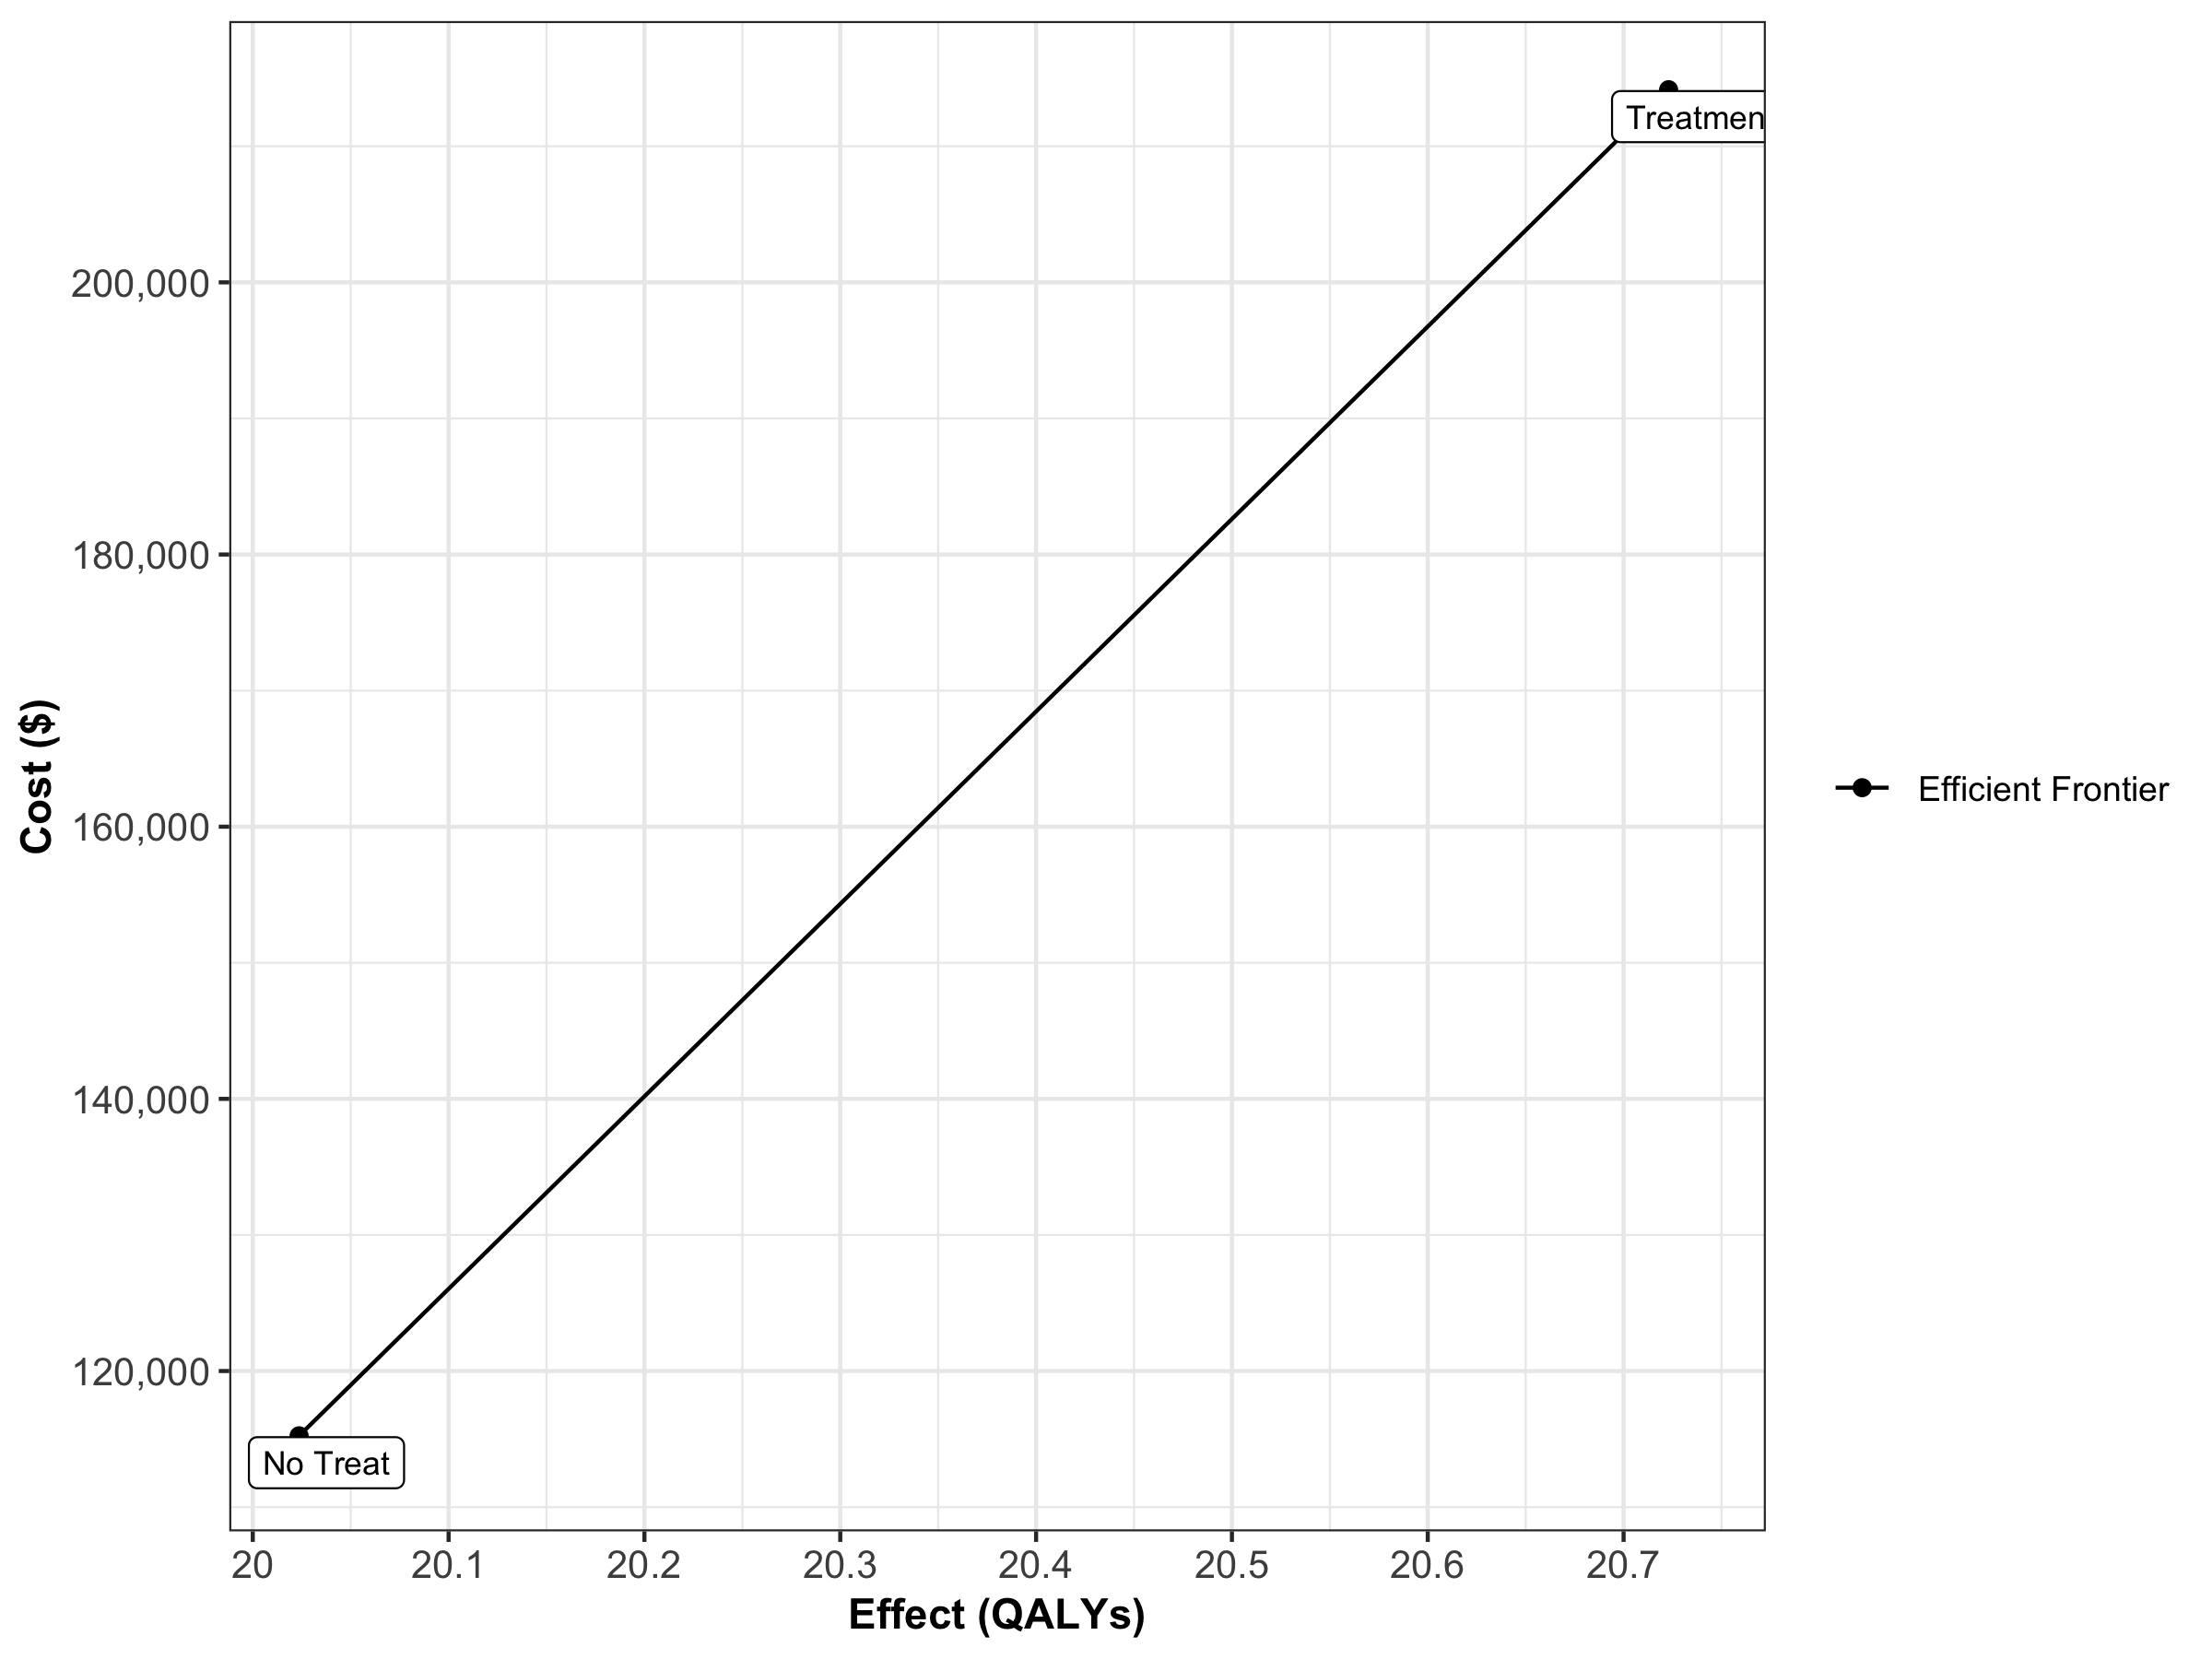
\includegraphics{../figs/05a_cea-frontier.png}
\caption{One-way sensitivity analysis results for the parameters c.Trt,
p.HS1, u.S1 and u.Trt \label{fig:05a_CEA-frontier}}
\end{figure}

We then conduct a series of deterministic sensitivity analysis. First,
we conduct a one-way sensitivity analysis (OWSA) on the variables
\texttt{c.Trt}, \texttt{p.HS1}, \texttt{u.S1} and \texttt{u.Trt} and a
two-way sensitivity analysis (TWSA) using the owsa\_det and twsa\_det
functions in the \emph{00\_general\_functions.R} file. We use the output
of these functions to produce different SA plots, such as OWSA tornado,
one-way optimal strategy and TWSA plots (Figures
\ref{fig:05a_owsa-nmb}{]} - \ref{fig:05a_twsa-uS1-uTrt-nmb.png}).

\begin{figure}
\centering
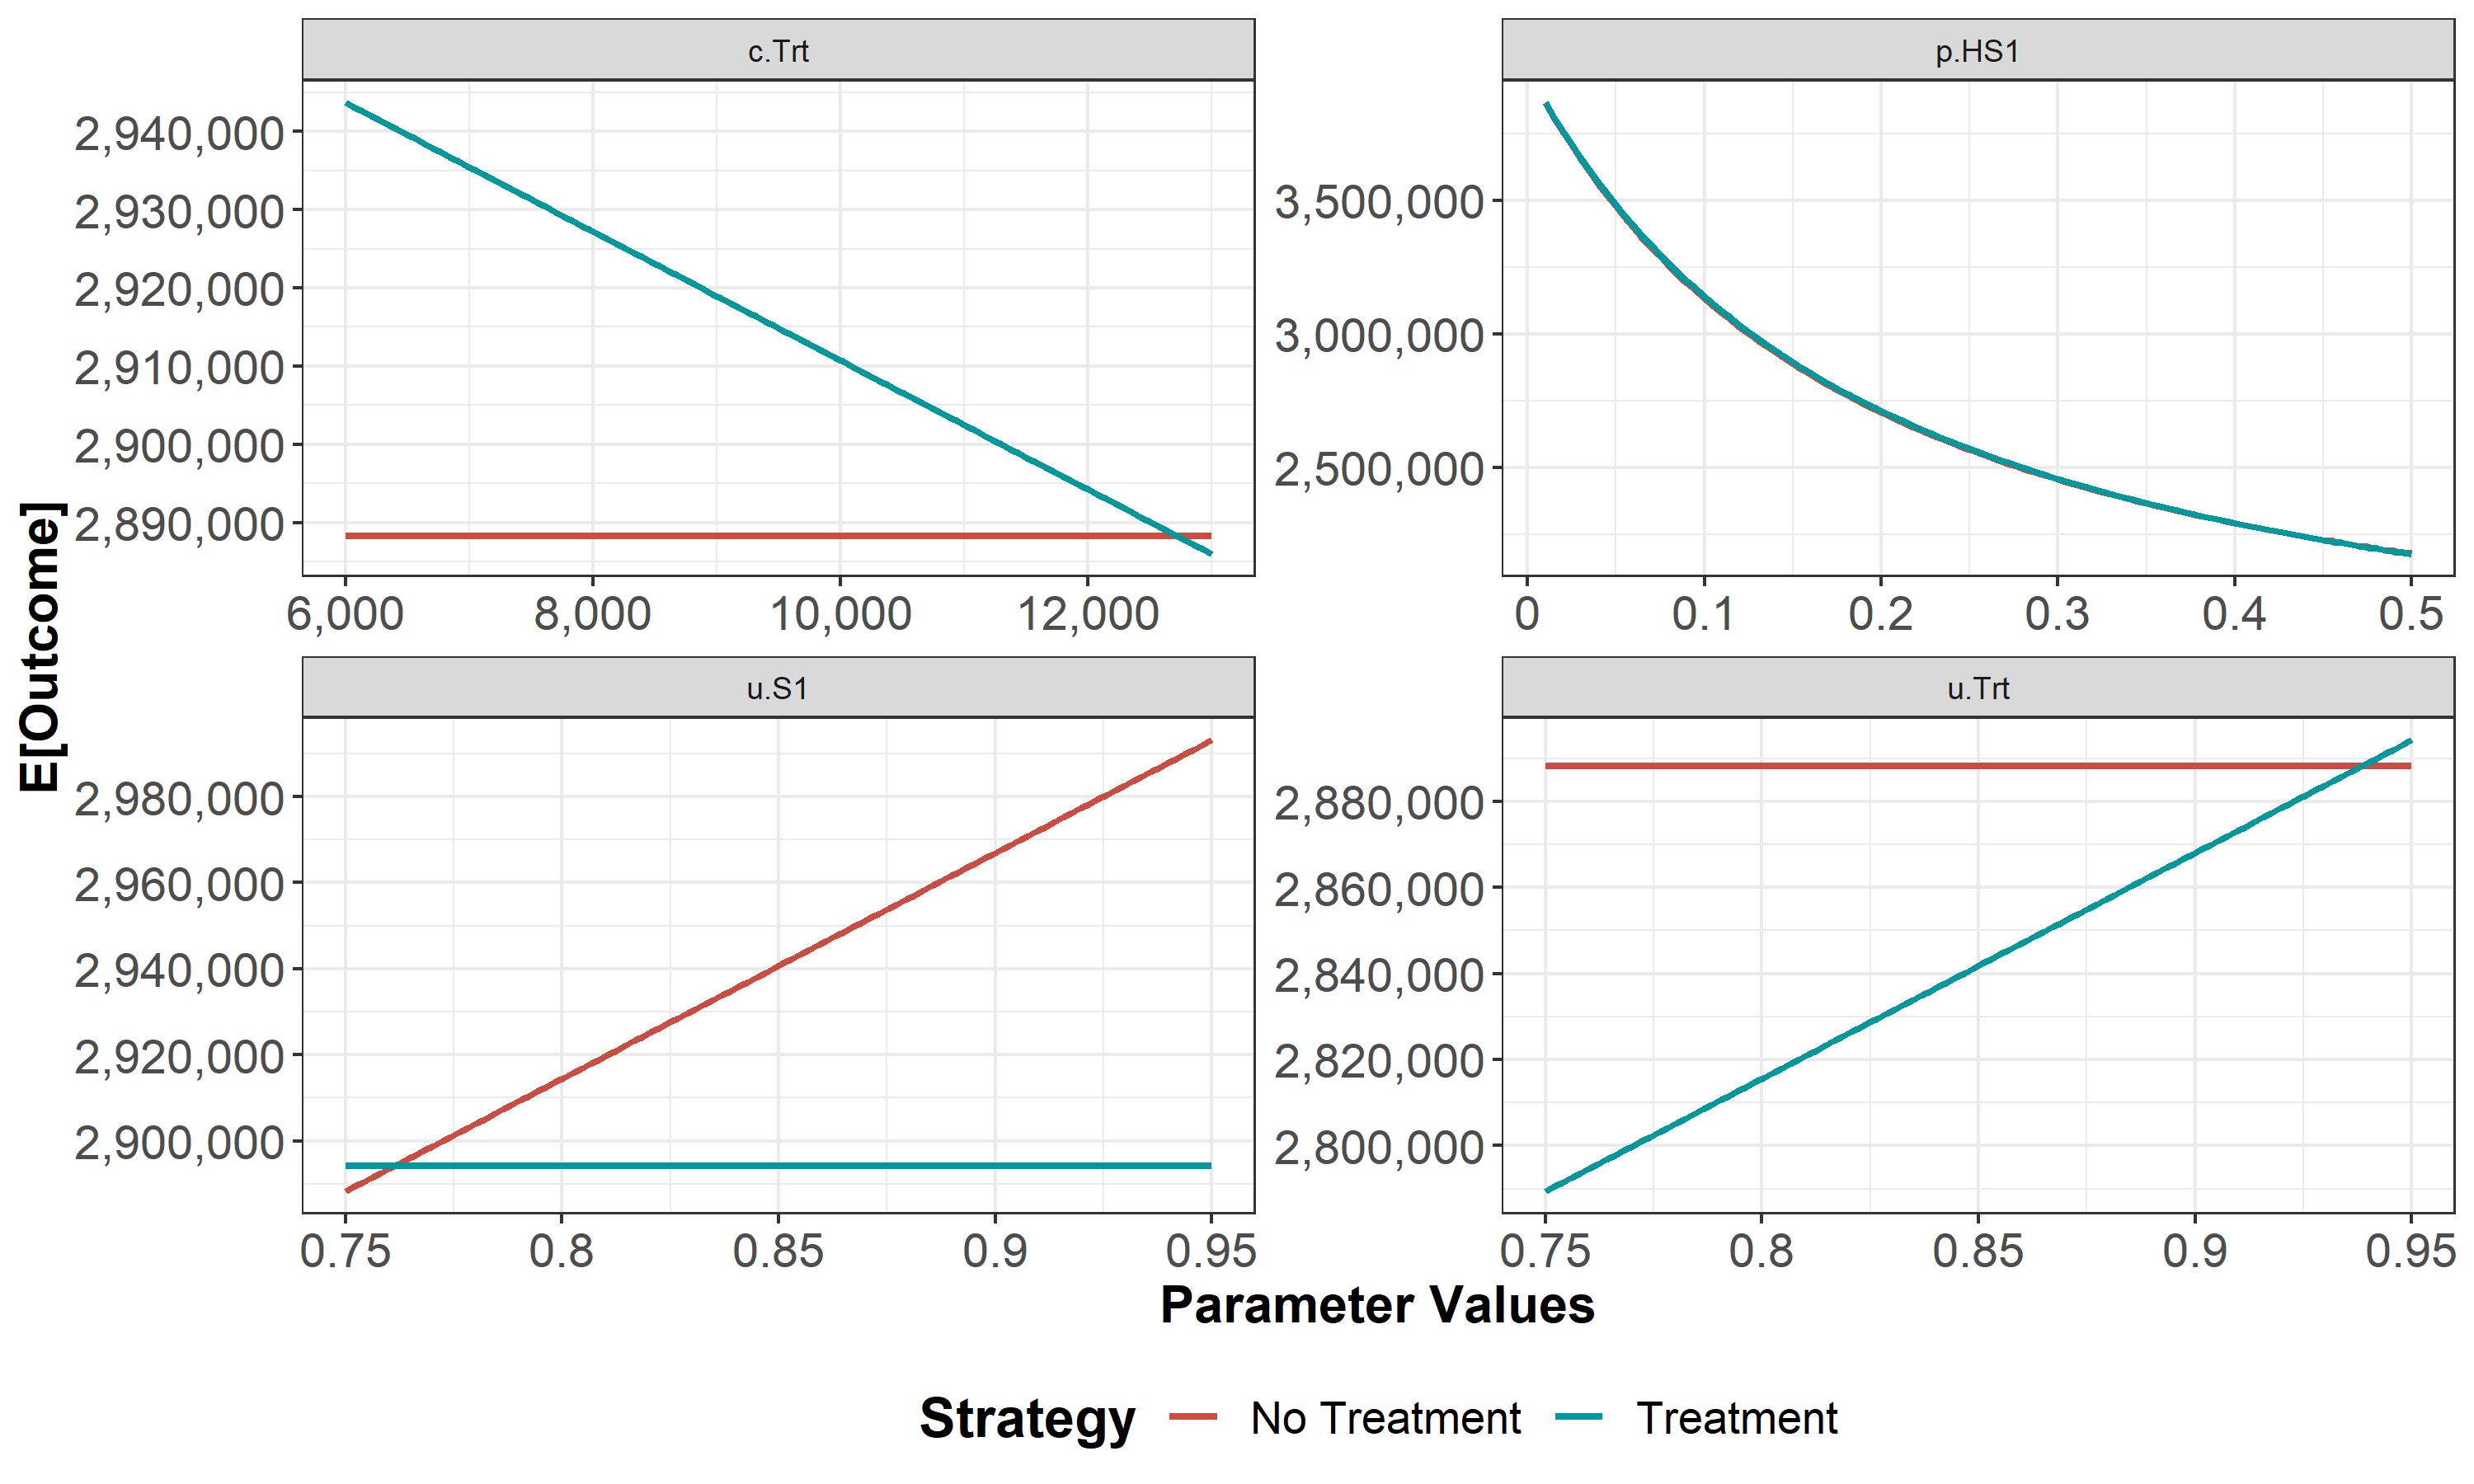
\includegraphics{../figs/05a_owsa-nmb.png}
\caption{One-way sensitivity analysis results for the parameters c.Trt,
p.HS1, u.S1 and u.Trt \label{fig:05a_owsa-nmb}}
\end{figure}

\begin{figure}
\centering
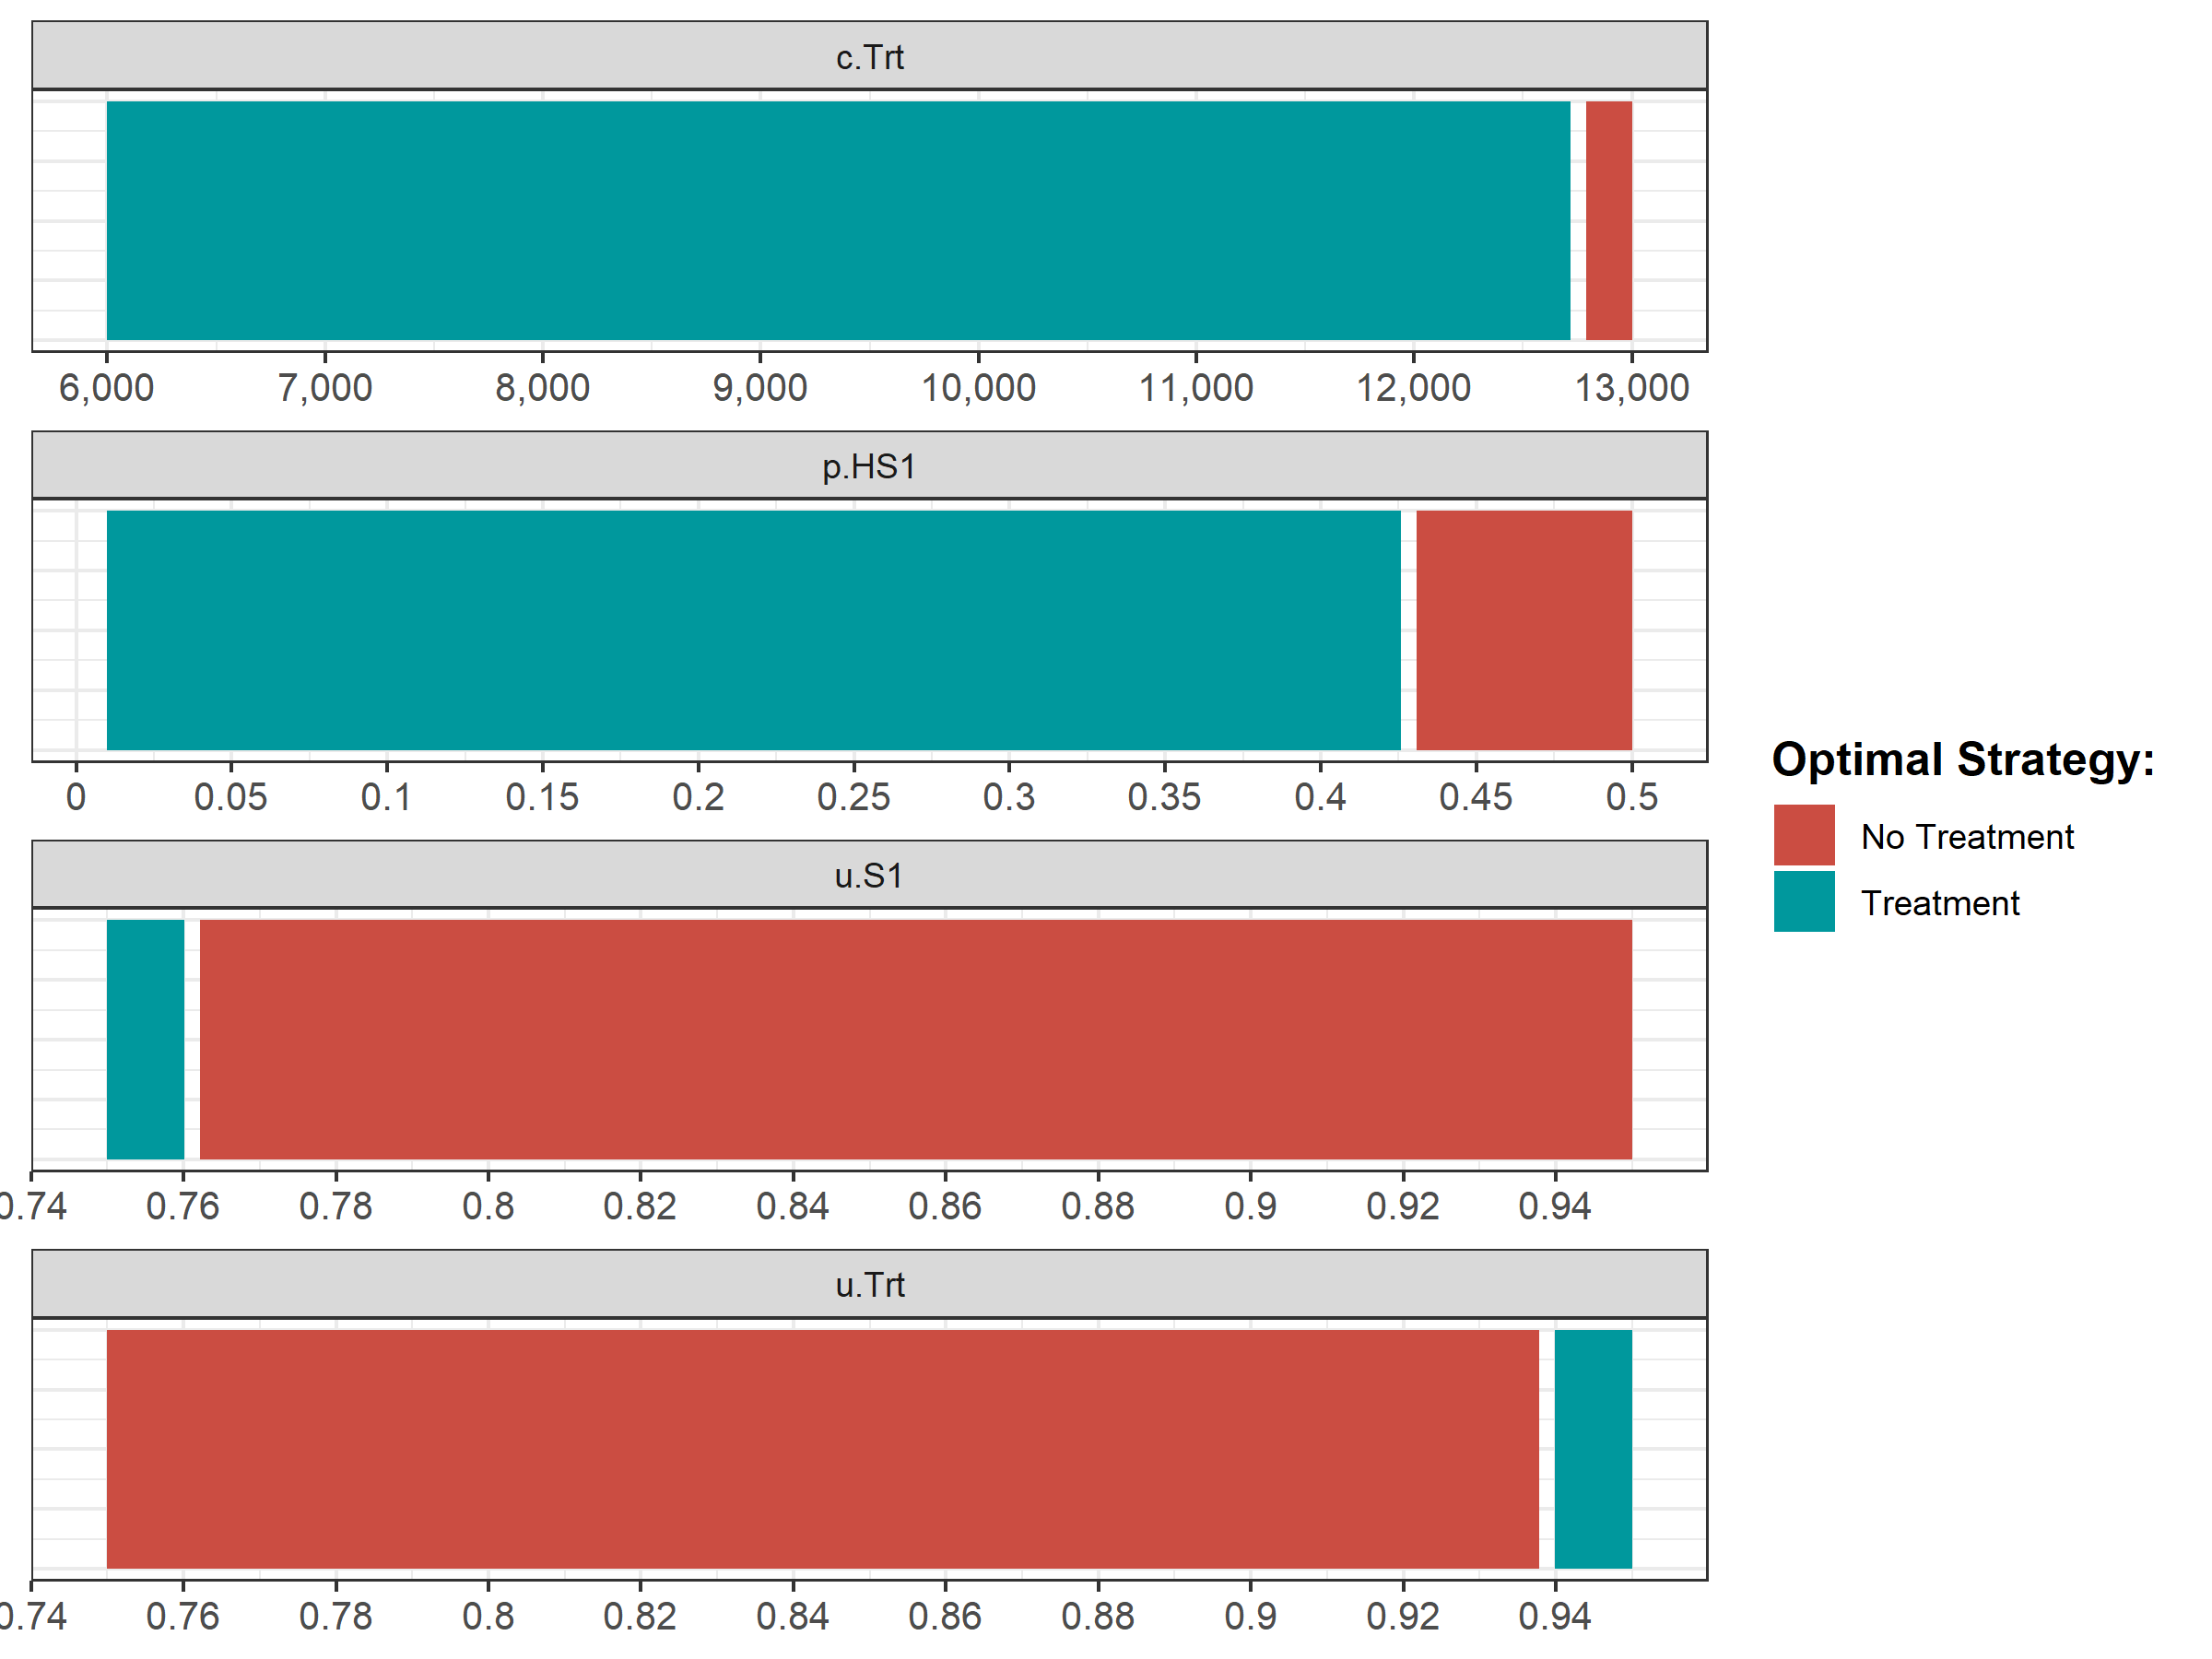
\includegraphics{../figs/05a_optimal-owsa-nmb.png}
\caption{The optimal strategy with OWSA
\label{fig:05a_optimal-owsa-nmb}}
\end{figure}

\begin{figure}
\centering
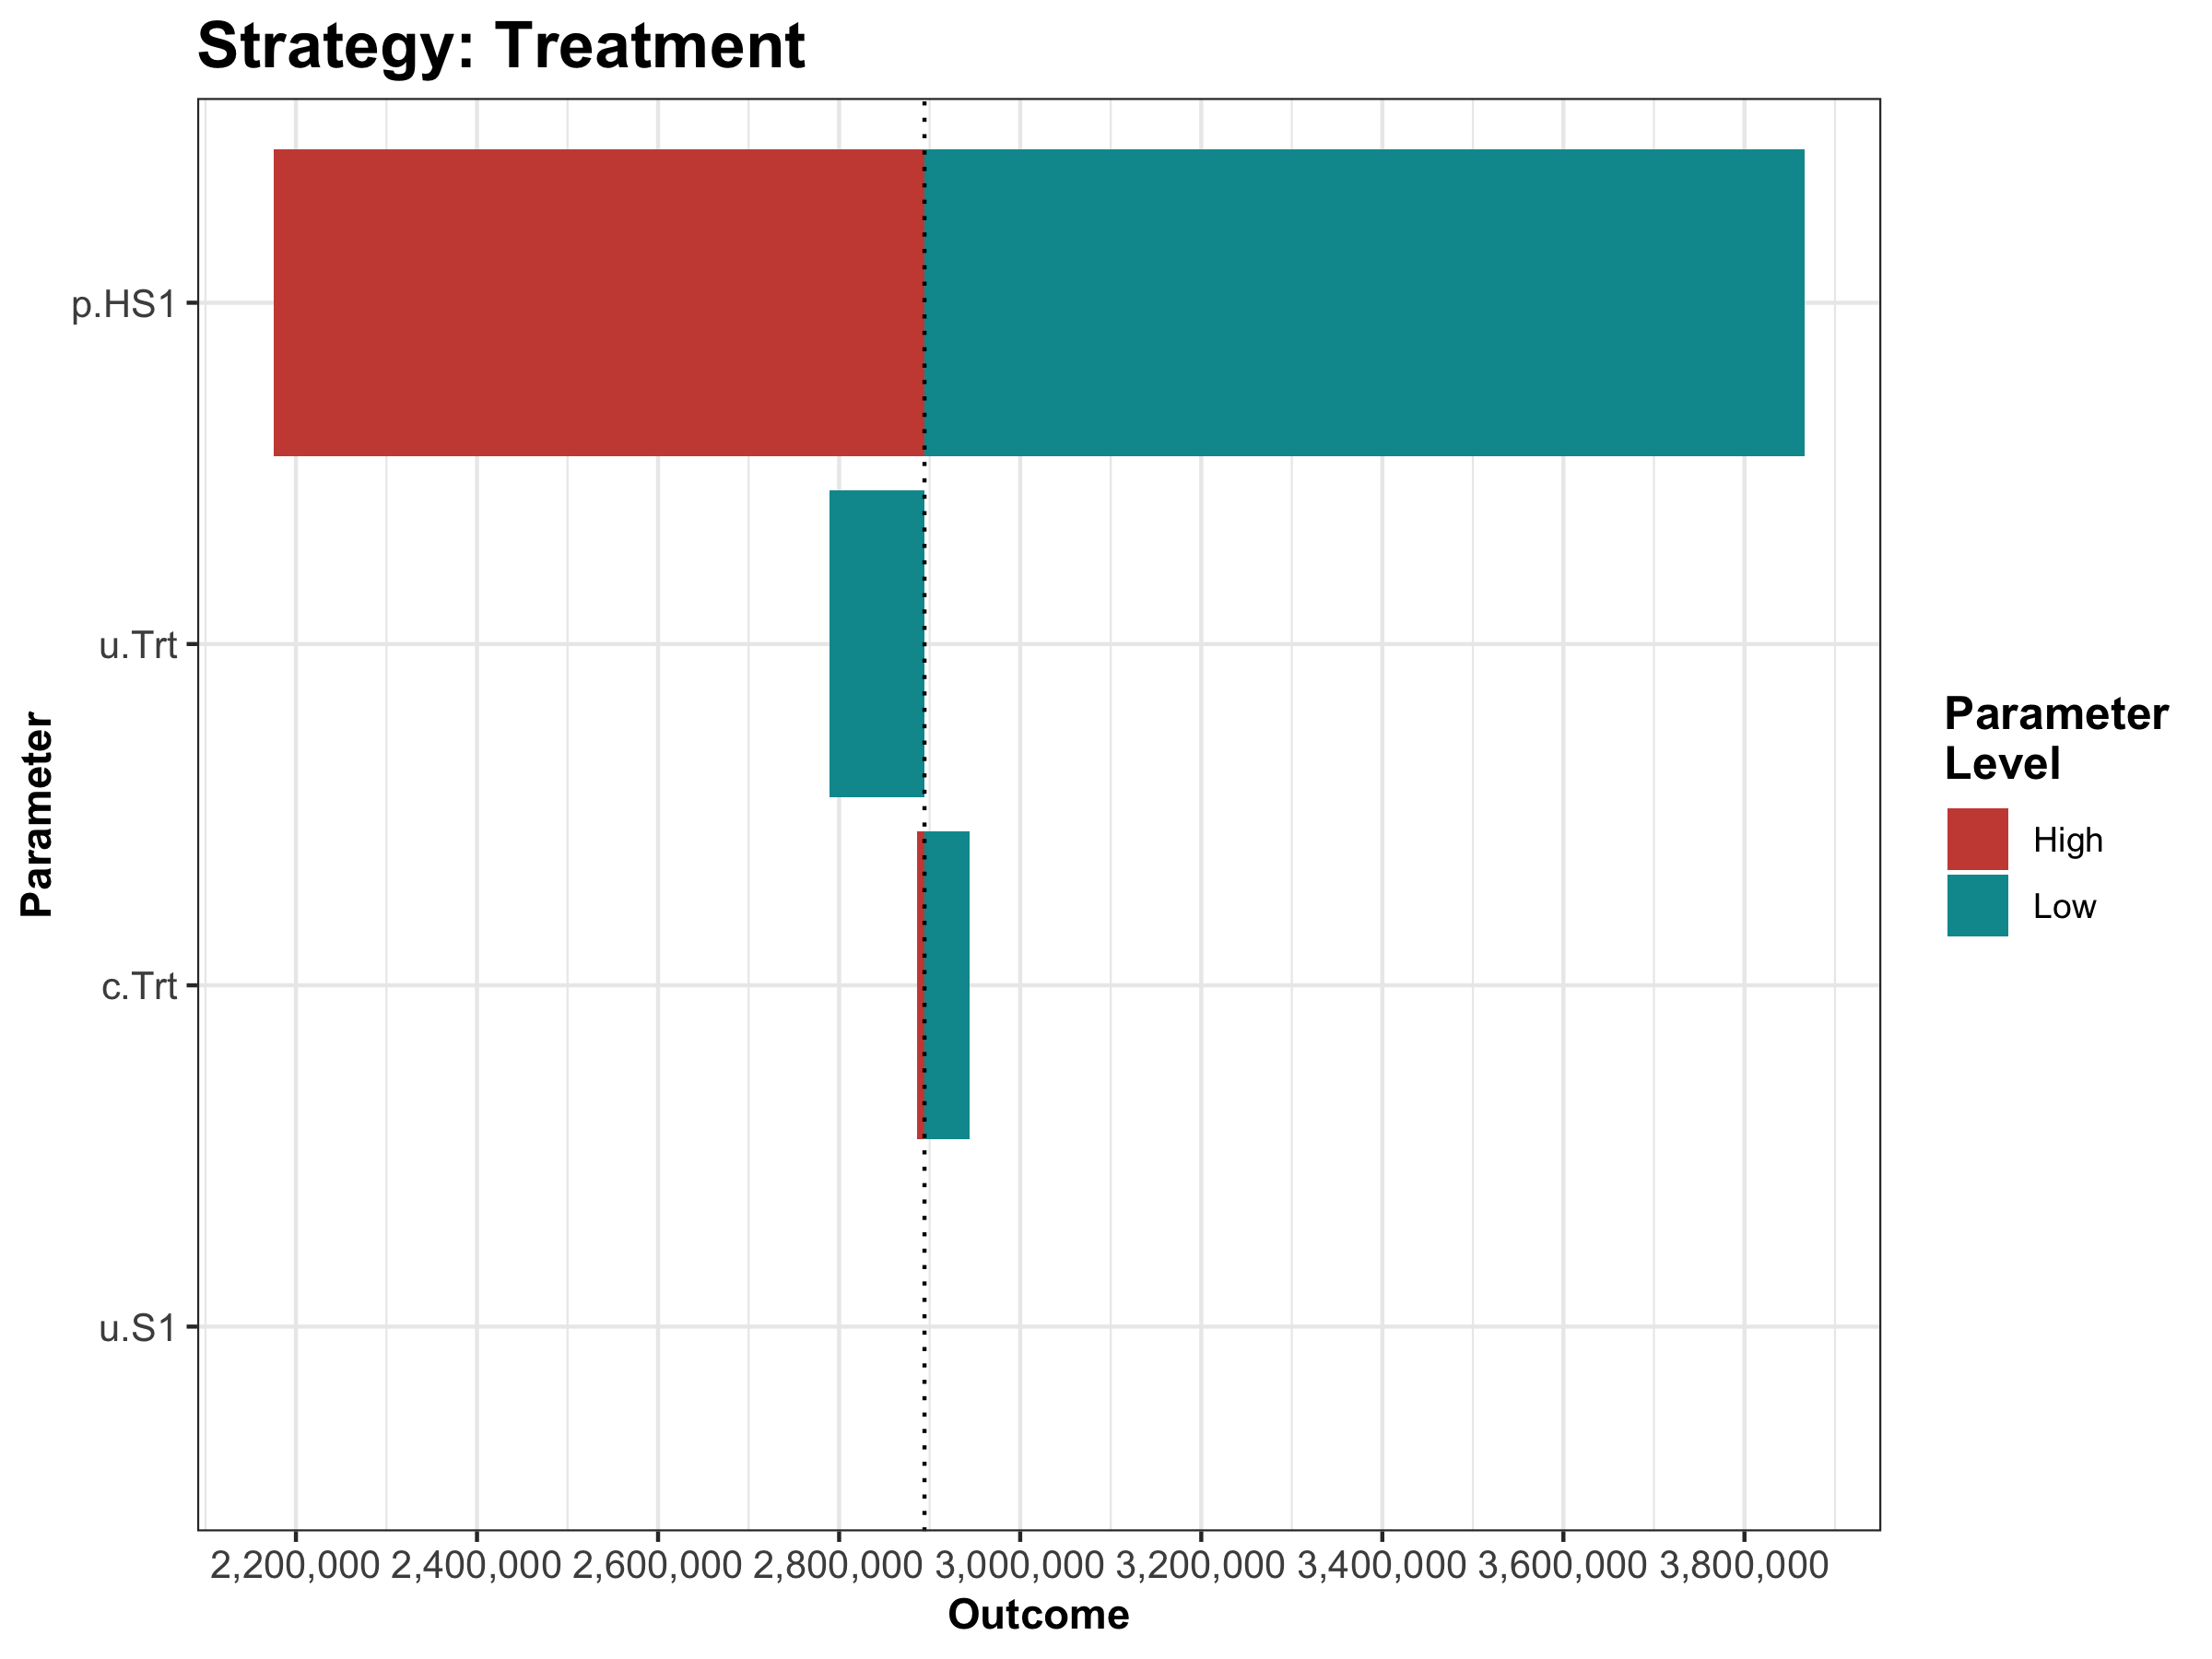
\includegraphics{../figs/05a_tornado-Treatment-nmb.png}
\caption{The tornado plot \label{fig:05a_tornado-Treatment-nmb}}
\end{figure}

\begin{figure}
\centering
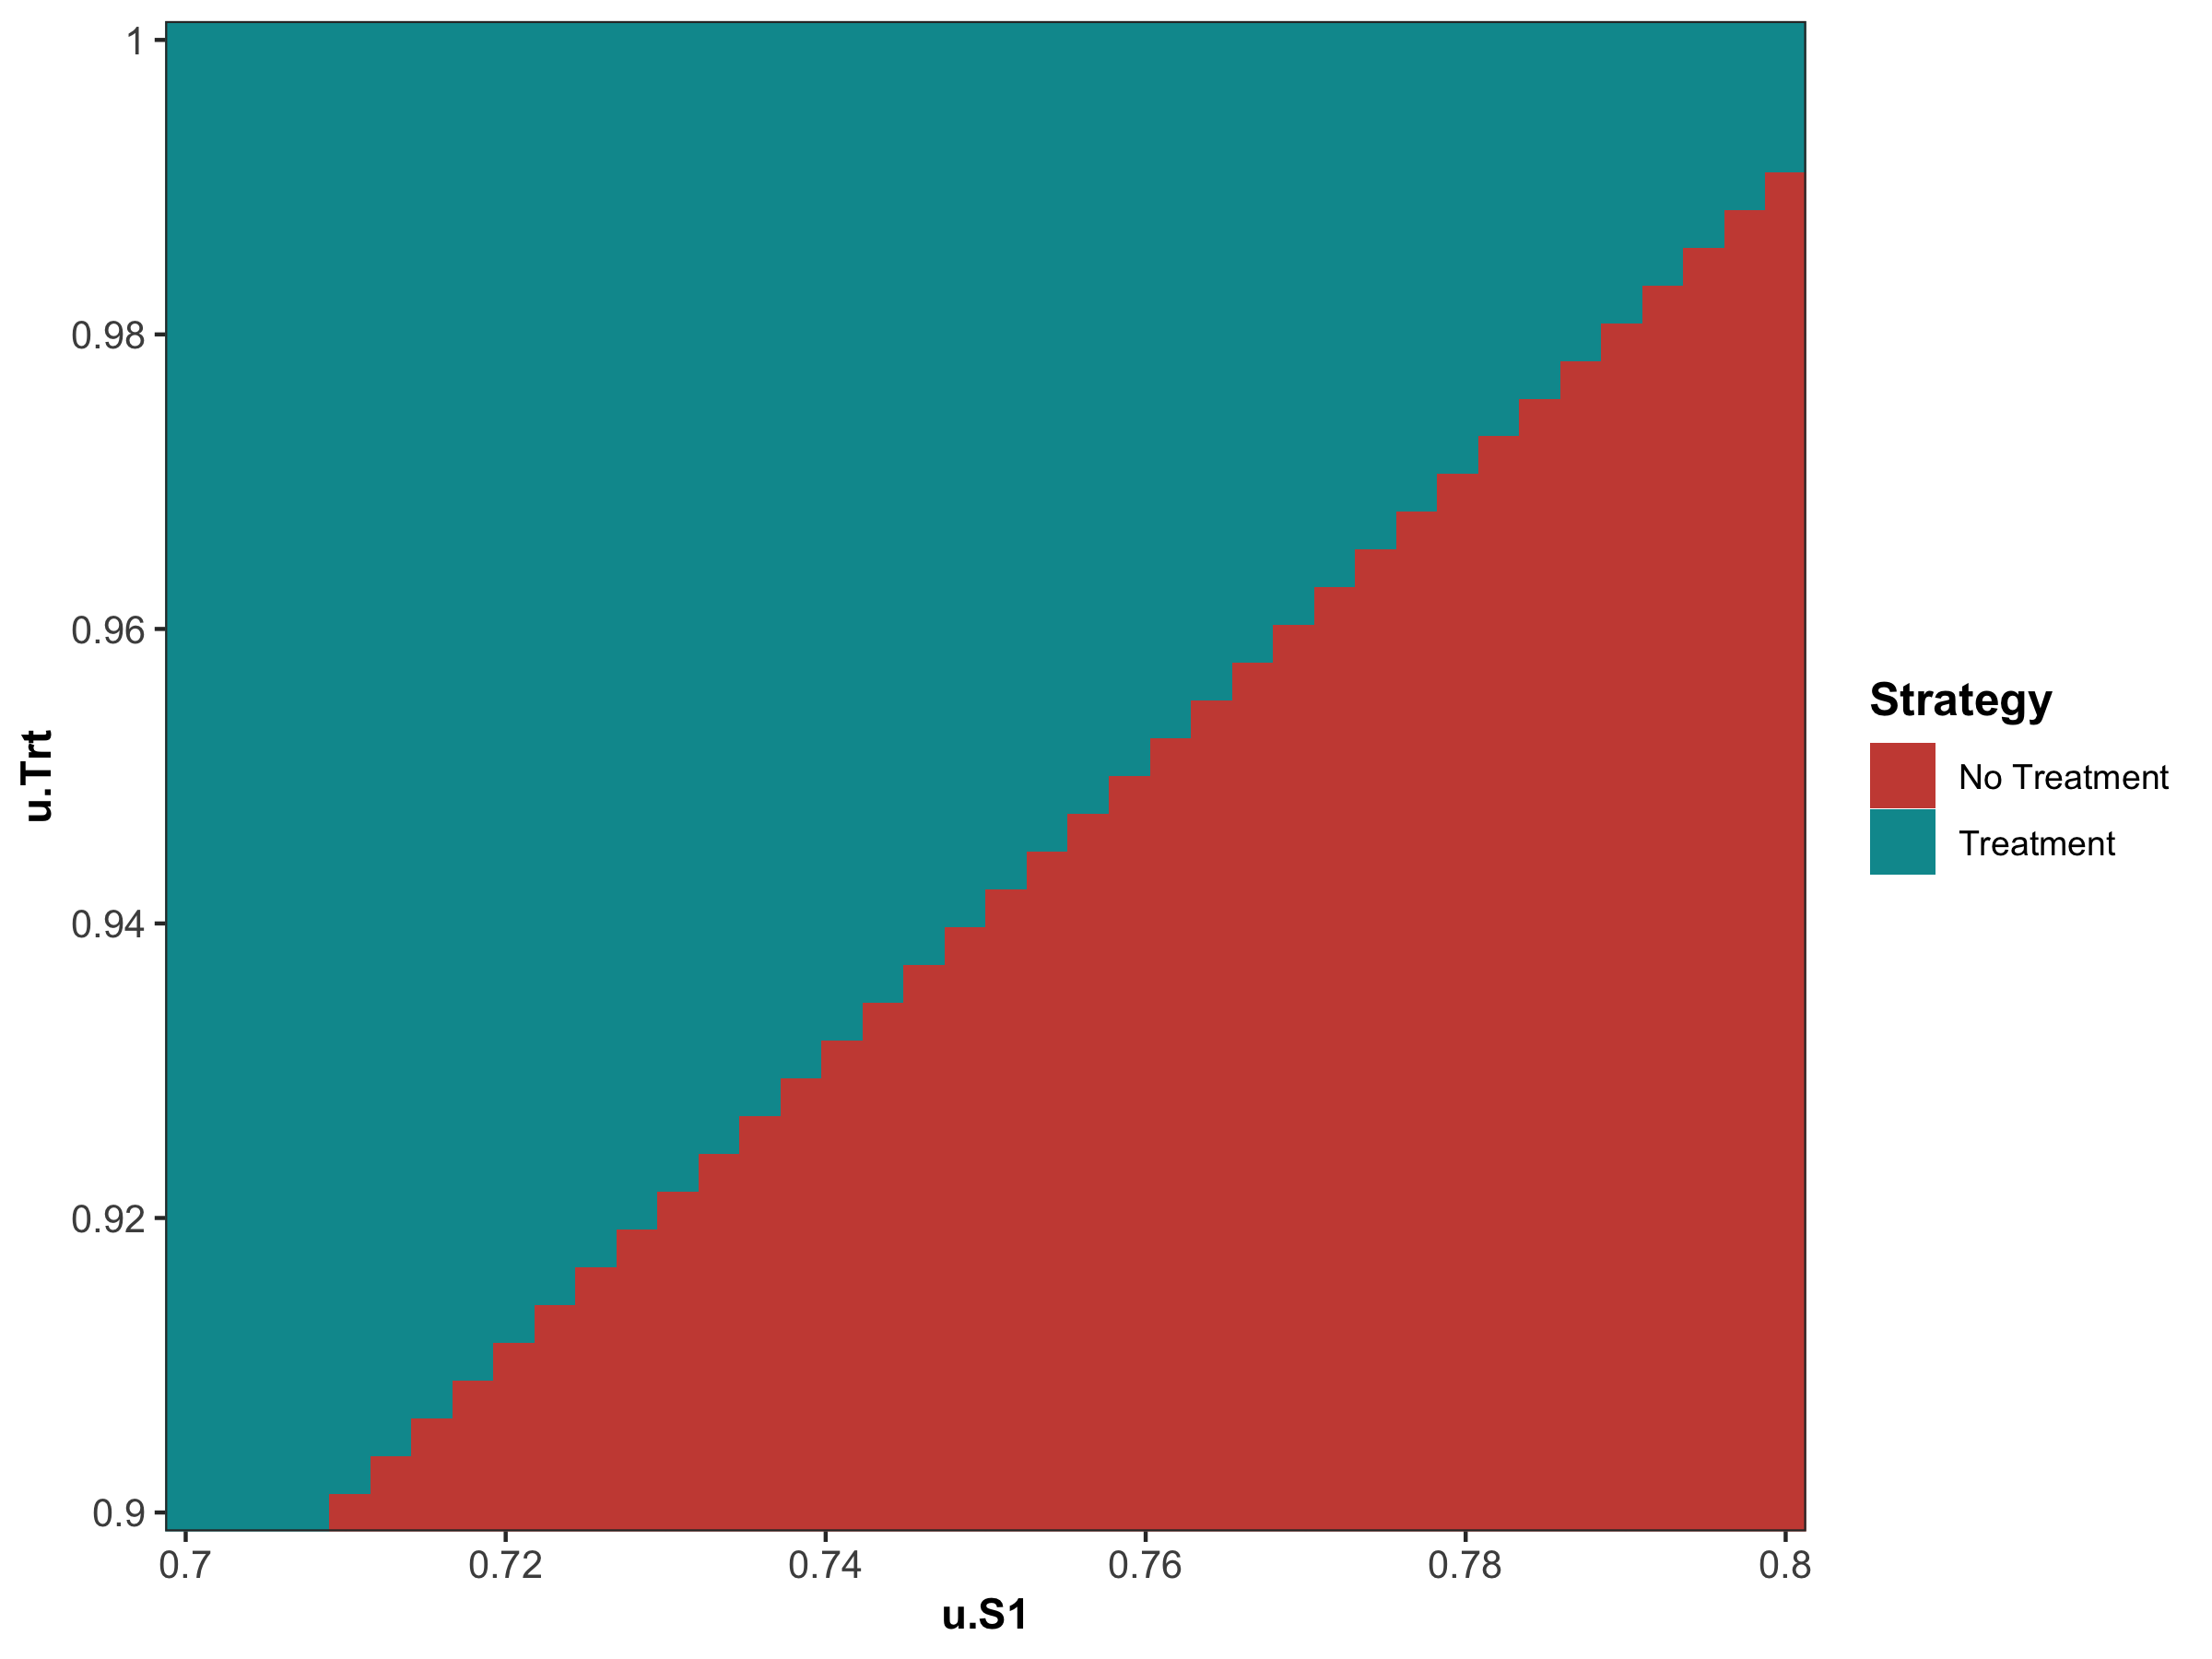
\includegraphics{../figs/05a_twsa-uS1-uTrt-nmb.png}
\caption{The two-way sensitivity results of the parameters u.Trt and
u.S1. \label{fig:05a_twsa-uS1-uTrt-nmb.png}}
\end{figure}

\paragraph{05b Uncertainty analysis}\label{b-uncertainty-analysis}

In this subcomponent, we evaluate decision uncertainty by propagating
the uncertainty through the CEA using probabilistic sensitivity analysis
(PSA). Until now we used the parameter values as described in Table
\ref{tab:parameters}. However, we are uncertain about these values. Most
of these input parameters are defined by probability distribution as
described in Table \ref{tab:parameters PSA}.

\begin{longtable}[]{@{}lcc@{}}
\caption{\label{tab:parameters PSA} Description of parameters with their
R name and distribution.}\tabularnewline
\toprule
\begin{minipage}[b]{0.43\columnwidth}\raggedright\strut
\textbf{Parameter}\strut
\end{minipage} & \begin{minipage}[b]{0.18\columnwidth}\centering\strut
\textbf{R name}\strut
\end{minipage} & \begin{minipage}[b]{0.20\columnwidth}\centering\strut
\textbf{Distribution}\strut
\end{minipage}\tabularnewline
\midrule
\endfirsthead
\toprule
\begin{minipage}[b]{0.43\columnwidth}\raggedright\strut
\textbf{Parameter}\strut
\end{minipage} & \begin{minipage}[b]{0.18\columnwidth}\centering\strut
\textbf{R name}\strut
\end{minipage} & \begin{minipage}[b]{0.20\columnwidth}\centering\strut
\textbf{Distribution}\strut
\end{minipage}\tabularnewline
\midrule
\endhead
\begin{minipage}[t]{0.43\columnwidth}\raggedright\strut
Annual transition probabilities\strut
\end{minipage} & \begin{minipage}[t]{0.18\columnwidth}\centering\strut
\strut
\end{minipage} & \begin{minipage}[t]{0.20\columnwidth}\centering\strut
\strut
\end{minipage}\tabularnewline
\begin{minipage}[t]{0.43\columnwidth}\raggedright\strut
- Disease onset (H to S1)\strut
\end{minipage} & \begin{minipage}[t]{0.18\columnwidth}\centering\strut
\texttt{p.HS1}\strut
\end{minipage} & \begin{minipage}[t]{0.20\columnwidth}\centering\strut
\texttt{beta(30,\ 170)}\strut
\end{minipage}\tabularnewline
\begin{minipage}[t]{0.43\columnwidth}\raggedright\strut
- Recovery (S1 to H)\strut
\end{minipage} & \begin{minipage}[t]{0.18\columnwidth}\centering\strut
\texttt{p.S1H}\strut
\end{minipage} & \begin{minipage}[t]{0.20\columnwidth}\centering\strut
\texttt{beta(60,\ 60)}\strut
\end{minipage}\tabularnewline
\begin{minipage}[t]{0.43\columnwidth}\raggedright\strut
Annual costs\strut
\end{minipage} & \begin{minipage}[t]{0.18\columnwidth}\centering\strut
\strut
\end{minipage} & \begin{minipage}[t]{0.20\columnwidth}\centering\strut
\strut
\end{minipage}\tabularnewline
\begin{minipage}[t]{0.43\columnwidth}\raggedright\strut
- Healthy individuals\strut
\end{minipage} & \begin{minipage}[t]{0.18\columnwidth}\centering\strut
\texttt{c.H}\strut
\end{minipage} & \begin{minipage}[t]{0.20\columnwidth}\centering\strut
\texttt{gamma(shape\ =\ 100,\ scale\ =\ 20)}\strut
\end{minipage}\tabularnewline
\begin{minipage}[t]{0.43\columnwidth}\raggedright\strut
- Sick individuals in S1\strut
\end{minipage} & \begin{minipage}[t]{0.18\columnwidth}\centering\strut
\texttt{c.S1}\strut
\end{minipage} & \begin{minipage}[t]{0.20\columnwidth}\centering\strut
\texttt{gamma(shape\ =\ 177.8,\ scale\ =\ 22.5)}\strut
\end{minipage}\tabularnewline
\begin{minipage}[t]{0.43\columnwidth}\raggedright\strut
- Sick individuals in S2\strut
\end{minipage} & \begin{minipage}[t]{0.18\columnwidth}\centering\strut
\texttt{c.S2}\strut
\end{minipage} & \begin{minipage}[t]{0.20\columnwidth}\centering\strut
\texttt{gamma(shape\ =\ 225,\ scale\ =\ 66.7)}\strut
\end{minipage}\tabularnewline
\begin{minipage}[t]{0.43\columnwidth}\raggedright\strut
- Additional costs of sick individuals treated in S1 or S2\strut
\end{minipage} & \begin{minipage}[t]{0.18\columnwidth}\centering\strut
\texttt{c.Trt}\strut
\end{minipage} & \begin{minipage}[t]{0.20\columnwidth}\centering\strut
\texttt{gamma(shape\ =\ 73.5,\ scale\ =\ 163.3)}\strut
\end{minipage}\tabularnewline
\begin{minipage}[t]{0.43\columnwidth}\raggedright\strut
Utility weights\strut
\end{minipage} & \begin{minipage}[t]{0.18\columnwidth}\centering\strut
\strut
\end{minipage} & \begin{minipage}[t]{0.20\columnwidth}\centering\strut
\strut
\end{minipage}\tabularnewline
\begin{minipage}[t]{0.43\columnwidth}\raggedright\strut
- Healthy individuals\strut
\end{minipage} & \begin{minipage}[t]{0.18\columnwidth}\centering\strut
\texttt{u.H}\strut
\end{minipage} & \begin{minipage}[t]{0.20\columnwidth}\centering\strut
\texttt{truncnorm(mean\ =\ 1,\ sd\ =\ 0.01,\ b\ =\ 1)}\strut
\end{minipage}\tabularnewline
\begin{minipage}[t]{0.43\columnwidth}\raggedright\strut
- Sick individuals in S1\strut
\end{minipage} & \begin{minipage}[t]{0.18\columnwidth}\centering\strut
\texttt{u.S1}\strut
\end{minipage} & \begin{minipage}[t]{0.20\columnwidth}\centering\strut
\texttt{truncnorm(mean\ =\ 0.75,\ sd\ =\ 0.02,\ b\ =\ 1)}\strut
\end{minipage}\tabularnewline
\begin{minipage}[t]{0.43\columnwidth}\raggedright\strut
- Sick individuals in S2\strut
\end{minipage} & \begin{minipage}[t]{0.18\columnwidth}\centering\strut
\texttt{u.S2}\strut
\end{minipage} & \begin{minipage}[t]{0.20\columnwidth}\centering\strut
\texttt{truncnorm(mean\ =\ 0.50,\ sd\ =\ 0.03,\ b\ =\ 1)}\strut
\end{minipage}\tabularnewline
\begin{minipage}[t]{0.43\columnwidth}\raggedright\strut
Intervention effect\strut
\end{minipage} & \begin{minipage}[t]{0.18\columnwidth}\centering\strut
\strut
\end{minipage} & \begin{minipage}[t]{0.20\columnwidth}\centering\strut
\strut
\end{minipage}\tabularnewline
\begin{minipage}[t]{0.43\columnwidth}\raggedright\strut
- Utility for treated individuals in S1\strut
\end{minipage} & \begin{minipage}[t]{0.18\columnwidth}\centering\strut
\texttt{u.Trt}\strut
\end{minipage} & \begin{minipage}[t]{0.20\columnwidth}\centering\strut
\texttt{truncnorm(mean\ =\ 0.95,\ sd\ =\ 0.02,\ b\ =\ 1)}\strut
\end{minipage}\tabularnewline
\bottomrule
\end{longtable}

In a PSA we sample the input parameter values from these distributions
and we then run the model at each sample. In the file
\emph{05b\_uncertainty-analysis\_functions.R} we created a single
function, called \texttt{f.generate\_psa\_params}, that generates a PSA
dataset for all the CEA input parameters. We specify the number of PSA
samples via the \texttt{n.sim} argument. The function also accepts
specifying a seed to allow reproducibility of the results.

\begin{Shaded}
\begin{Highlighting}[]
\KeywordTok{print.function}\NormalTok{(f.generate_psa_params) }\CommentTok{# print the function }
\end{Highlighting}
\end{Shaded}

\begin{verbatim}
## function (n.sim, seed = 20190220) 
## {
##     load("output/03_imis-output.RData")
##     n.sim <- nrow(m.calib.post)
##     set.seed <- seed
##     df.psa.params <- data.frame(m.calib.post, p.HS1 = rbeta(n.sim, 
##         30, 170), p.S1H = rbeta(n.sim, 60, 60), c.H = rgamma(n.sim, 
##         shape = 100, scale = 20), c.S1 = rgamma(n.sim, shape = 177.8, 
##         scale = 22.5), c.S2 = rgamma(n.sim, shape = 225, scale = 66.7), 
##         c.Trt = rgamma(n.sim, shape = 73.5, scale = 163.3), c.D = 0, 
##         u.H = rtruncnorm(n.sim, mean = 1, sd = 0.01, b = 1), 
##         u.S1 = rtruncnorm(n.sim, mean = 0.75, sd = 0.02, b = 1), 
##         u.S2 = rtruncnorm(n.sim, mean = 0.5, sd = 0.03, b = 1), 
##         u.D = 0, u.Trt = rtruncnorm(n.sim, mean = 0.95, sd = 0.02, 
##             b = 1))
##     return(df.psa.params)
## }
## <bytecode: 0x7fa07ef88e80>
\end{verbatim}

The function returns the \texttt{df.psa.input} dataframe with a PSA
dataset of the input parameters. With this dataframe we can run the PSA
to produce distributions of costs, effectiveness and NMB. The PSA is
performed by the \emph{05b\_probabilistic-analysis.R} script. As shown
in the code below, the \texttt{df.psa.input} dataframe is used by the
\texttt{f.update\_param\_list} function to generate the corresponding
list of parameters for the PSA. For each simulation, we perfrom three
steps. First, the list of parameters is updated by the
\texttt{f.update\_param\_list} function. Second, the model is executed
by the \texttt{f.calculate\_ce\_out} function using the updated
parameter list and third, the dataframes \texttt{df.c} and \texttt{df.e}
store the estimated cost and effects, respectively. The final part of
this loop is to satisfy the modeler when waiting on the results, by
displaying the simulation progress.

\begin{Shaded}
\begin{Highlighting}[]
\ControlFlowTok{for}\NormalTok{(i }\ControlFlowTok{in} \DecValTok{1}\OperatorTok{:}\NormalTok{n.sim)\{ }
\NormalTok{  l.psa.input <-}\StringTok{ }\KeywordTok{f.update_param_list}\NormalTok{(l.params.all, df.psa.input[i,])}
\NormalTok{  df.out.temp <-}\StringTok{ }\KeywordTok{f.calculate_ce_out}\NormalTok{(l.psa.input)}
\NormalTok{  df.c[i, ] <-}\StringTok{ }\NormalTok{df.out.temp}\OperatorTok{$}\NormalTok{Cost}
\NormalTok{  df.e[i, ] <-}\StringTok{ }\NormalTok{df.out.temp}\OperatorTok{$}\NormalTok{Effect}
  \CommentTok{# Display simulation progress}
  \ControlFlowTok{if}\NormalTok{(i}\OperatorTok{/}\NormalTok{(n.sim}\OperatorTok{/}\DecValTok{10}\NormalTok{) }\OperatorTok{==}\StringTok{ }\KeywordTok{round}\NormalTok{(i}\OperatorTok{/}\NormalTok{(n.sim}\OperatorTok{/}\DecValTok{10}\NormalTok{),}\DecValTok{0}\NormalTok{)) \{}
    \KeywordTok{cat}\NormalTok{(}\StringTok{'}\CharTok{\textbackslash{}r}\StringTok{'}\NormalTok{, }\KeywordTok{paste}\NormalTok{(i}\OperatorTok{/}\NormalTok{n.sim }\OperatorTok{*}\StringTok{ }\DecValTok{100}\NormalTok{, }\StringTok{"% done"}\NormalTok{, }\DataTypeTok{sep =} \StringTok{" "}\NormalTok{))}
\NormalTok{  \}}
\NormalTok{\}}
\end{Highlighting}
\end{Shaded}

We can plot the results using the \texttt{plot} function from
\texttt{dampack}. Figure \ref{fig:05b_CEAplane} shows the CE scatter
plot with the joint distribution of costs and effects for each strategy
and their corresponding 95\% confidence ellipse.

\begin{figure}
\centering
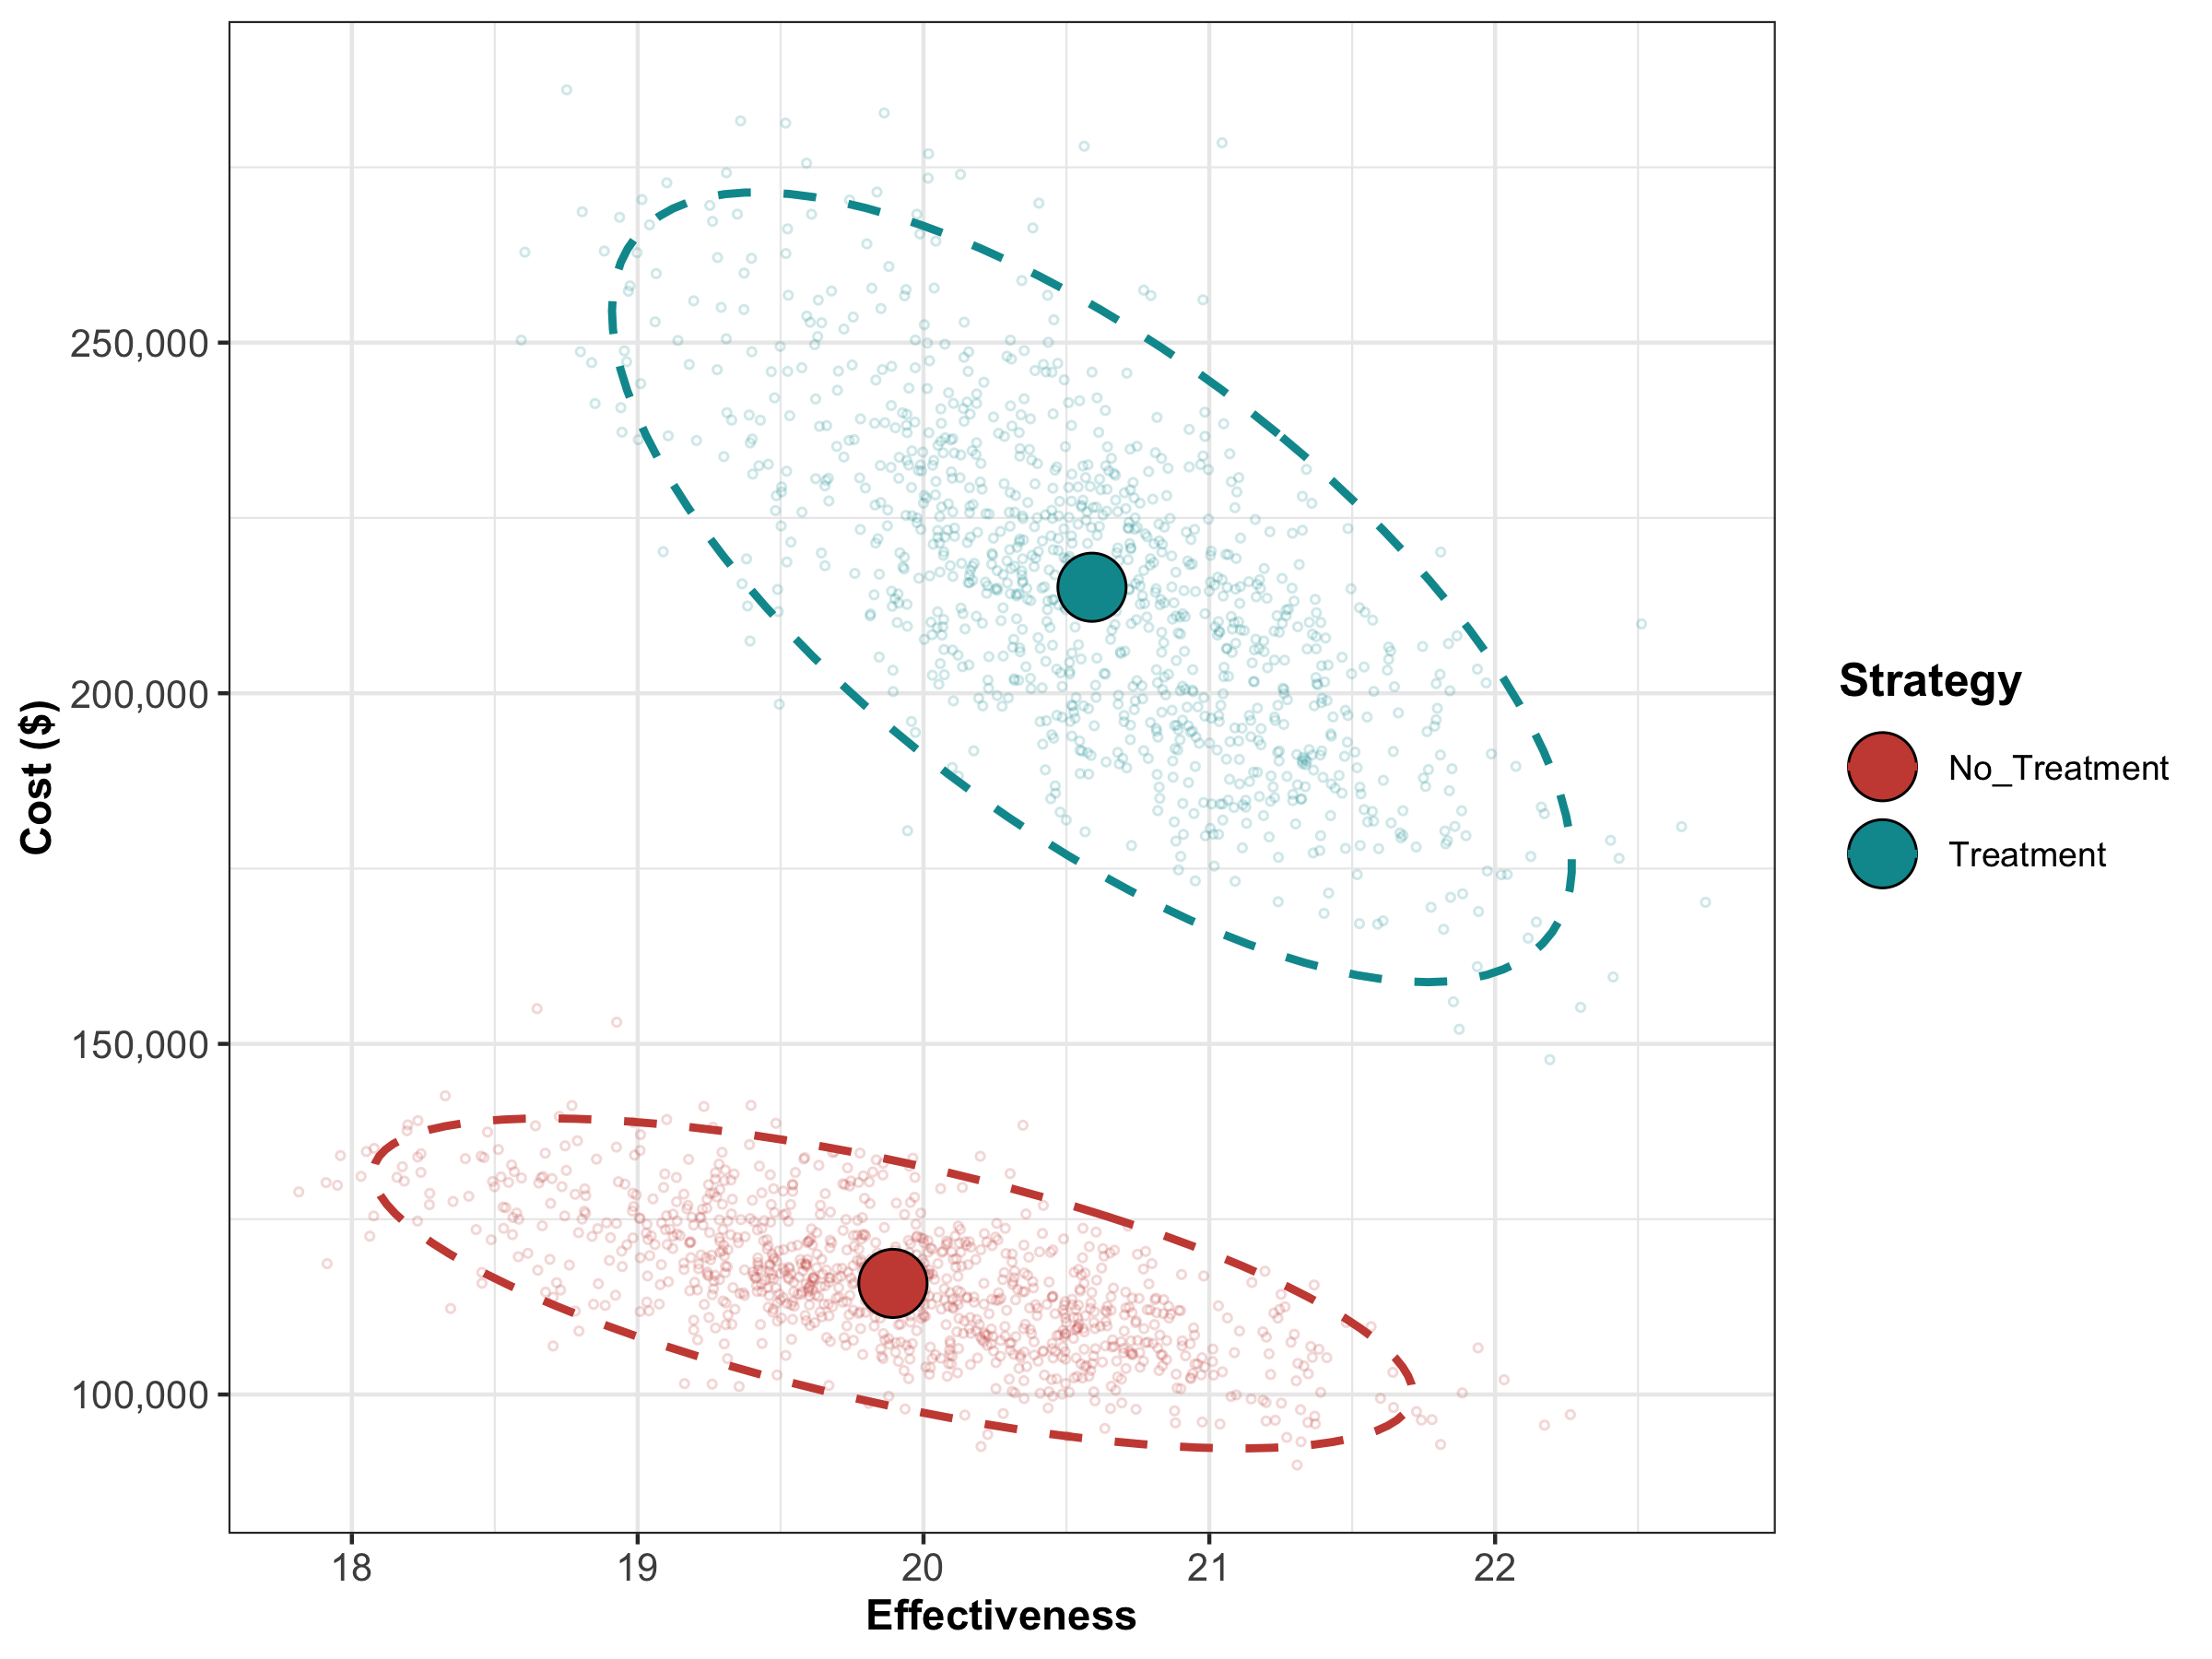
\includegraphics{../figs/05b_cea-plane-scatter.png}
\caption{The cost-effectiveness plane graph showing the results of the
probabilistic sensitivity analysis for the Sick-Sicker case-study.
\label{fig:05b_CEAplane}}
\end{figure}

\begin{table}[t]

\caption{\label{tab:unnamed-chunk-21}Probabilistic cost-effectiveness analysis results of the Sick-Sicker model comparing no treatment with treatment. \label{tab:df.cea.prob}}
\centering
\begin{tabular}{l|r|r|r|r|r}
\hline
Strategy & Cost & Effect & Inc\_Cost & Inc\_Effect & ICER\\
\hline
No\_Treatment & 115562.1 & 19.91203 & NA & NA & NA\\
\hline
Treatment & 214583.9 & 20.60653 & 99021.74 & 0.6944993 & 142580\\
\hline
\end{tabular}
\end{table}

Next, we perform a CEA using the previously used
\texttt{calculate\_icers} functions from \texttt{dampack}. Table
\ref{tab:df.cea.prob} shows the results of the probabilistic CEA. In
addition, we plot a cost-effectiveness plane with the frontier, the
cost-effectiveness acceptability curves (CEACs) and frontier (CEAF),
expected Loss curves (ELCs) (Figure \ref{fig:05b_cea-frontier-psa} -
\ref{fig:05b_elc}) (Alarid-Escudero et al. 2019). Followed by creating
linear regression metamodeling sensitivity analysis graphs (Figure
\ref{fig:05b_owsa-lrm-nmb} - \ref{fig:05b_twsa-lrm-uS1-uTrt-nmb}). All
generated figures are shown below and stored to the \emph{figs} folder
(H. Jalal et al. 2013).

\begin{figure}
\centering
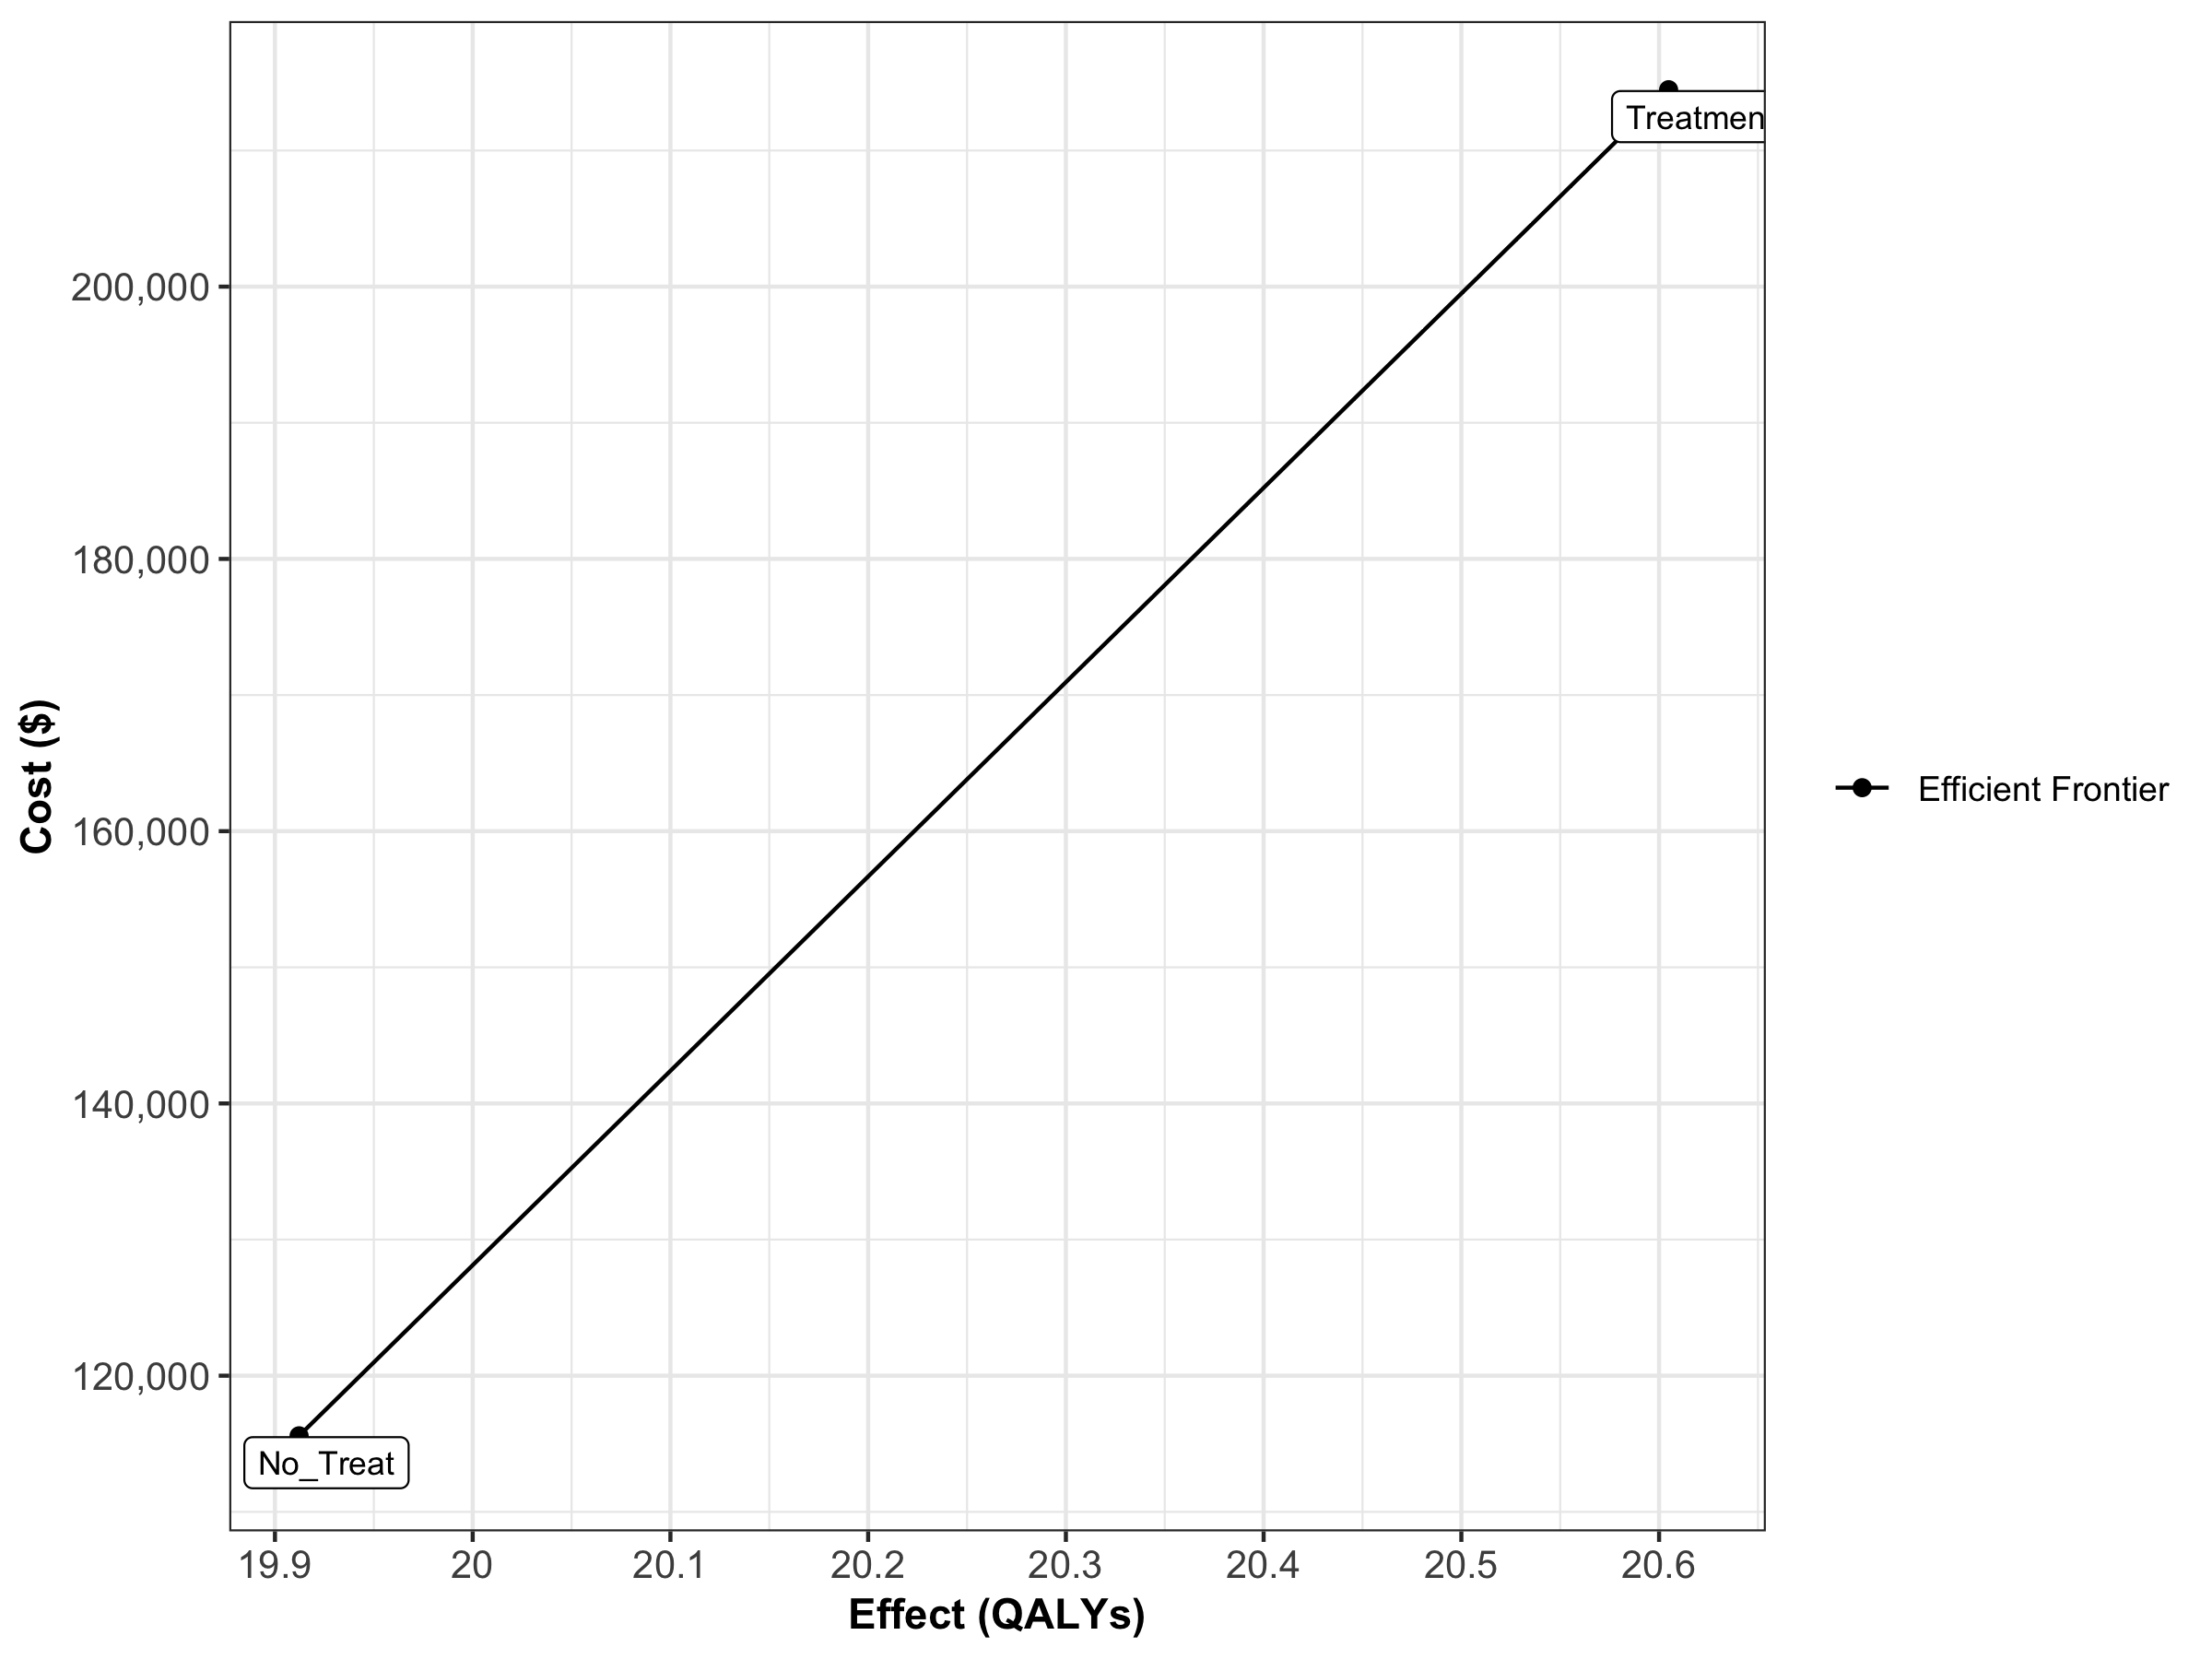
\includegraphics{../figs/05b_cea-frontier-psa.png}
\caption{Cost-effectiveness frontier\label{fig:05b_cea-frontier-psa}}
\end{figure}

\begin{figure}
\centering
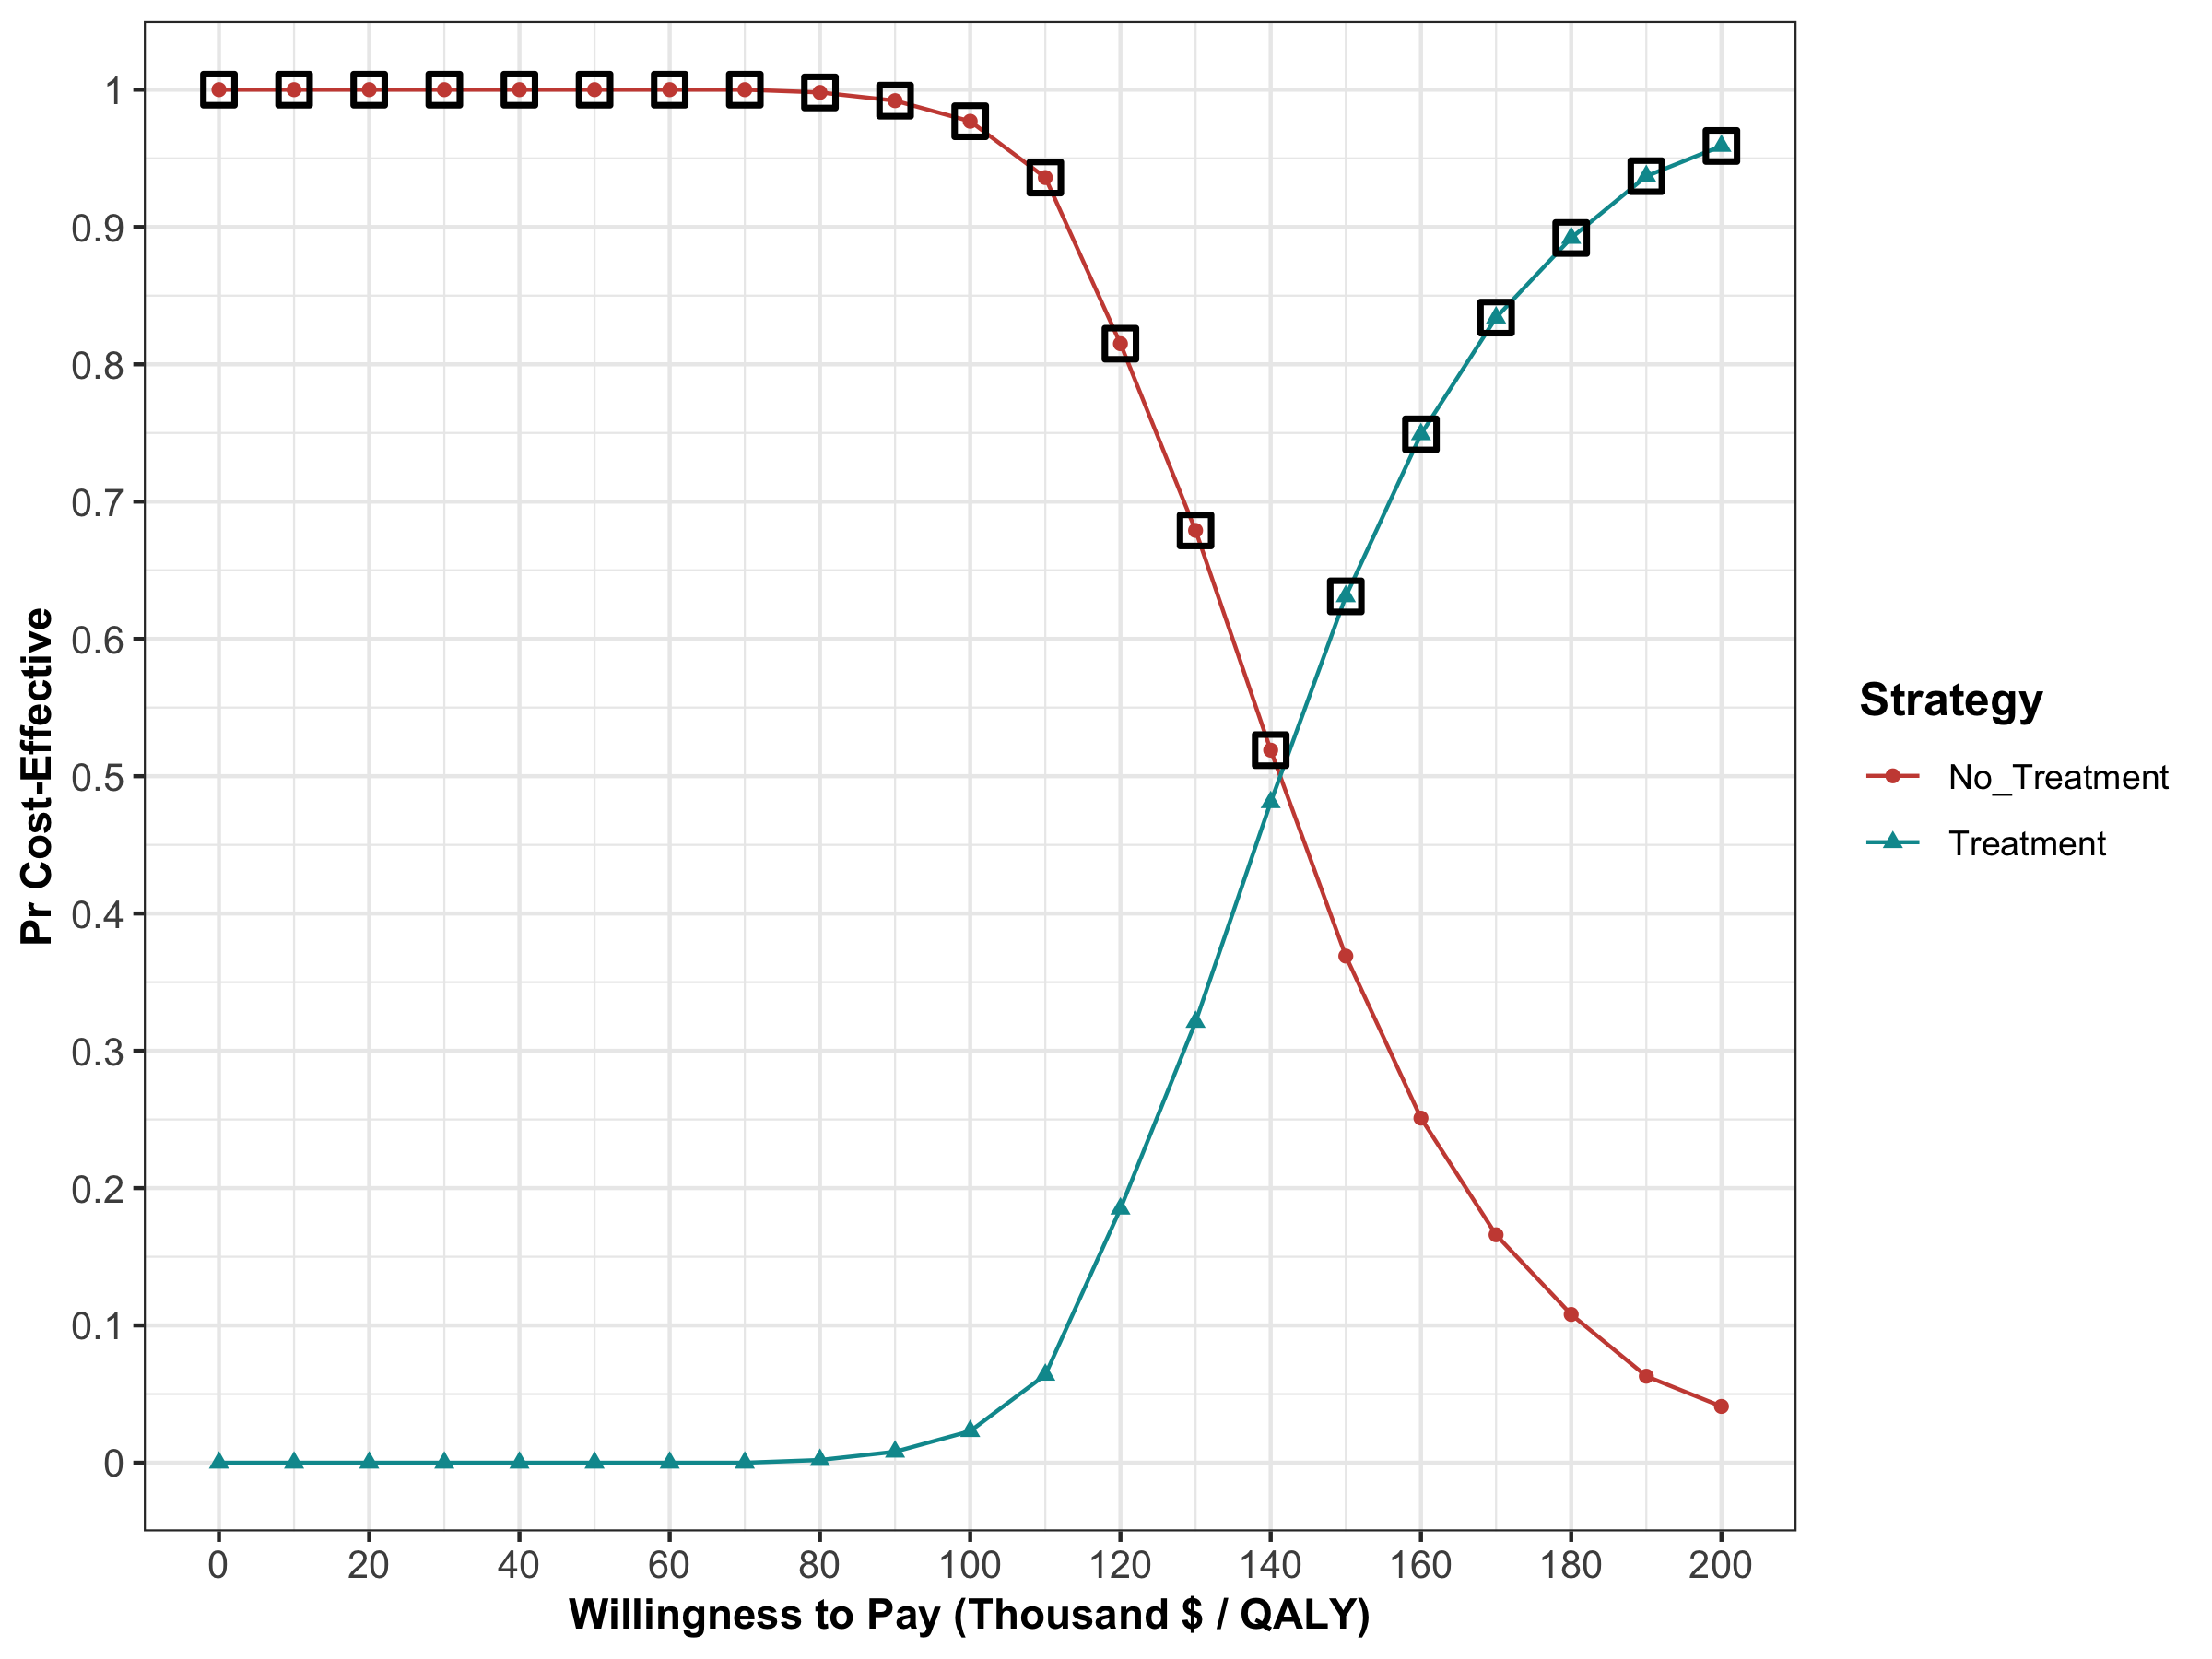
\includegraphics{../figs/05b_ceac-ceaf.png}
\caption{Cost-effectiveness acceptability curves (CEACs) and frontier
(CEAF)\label{fig:05b_ceac-ceaf}}
\end{figure}

\begin{figure}
\centering
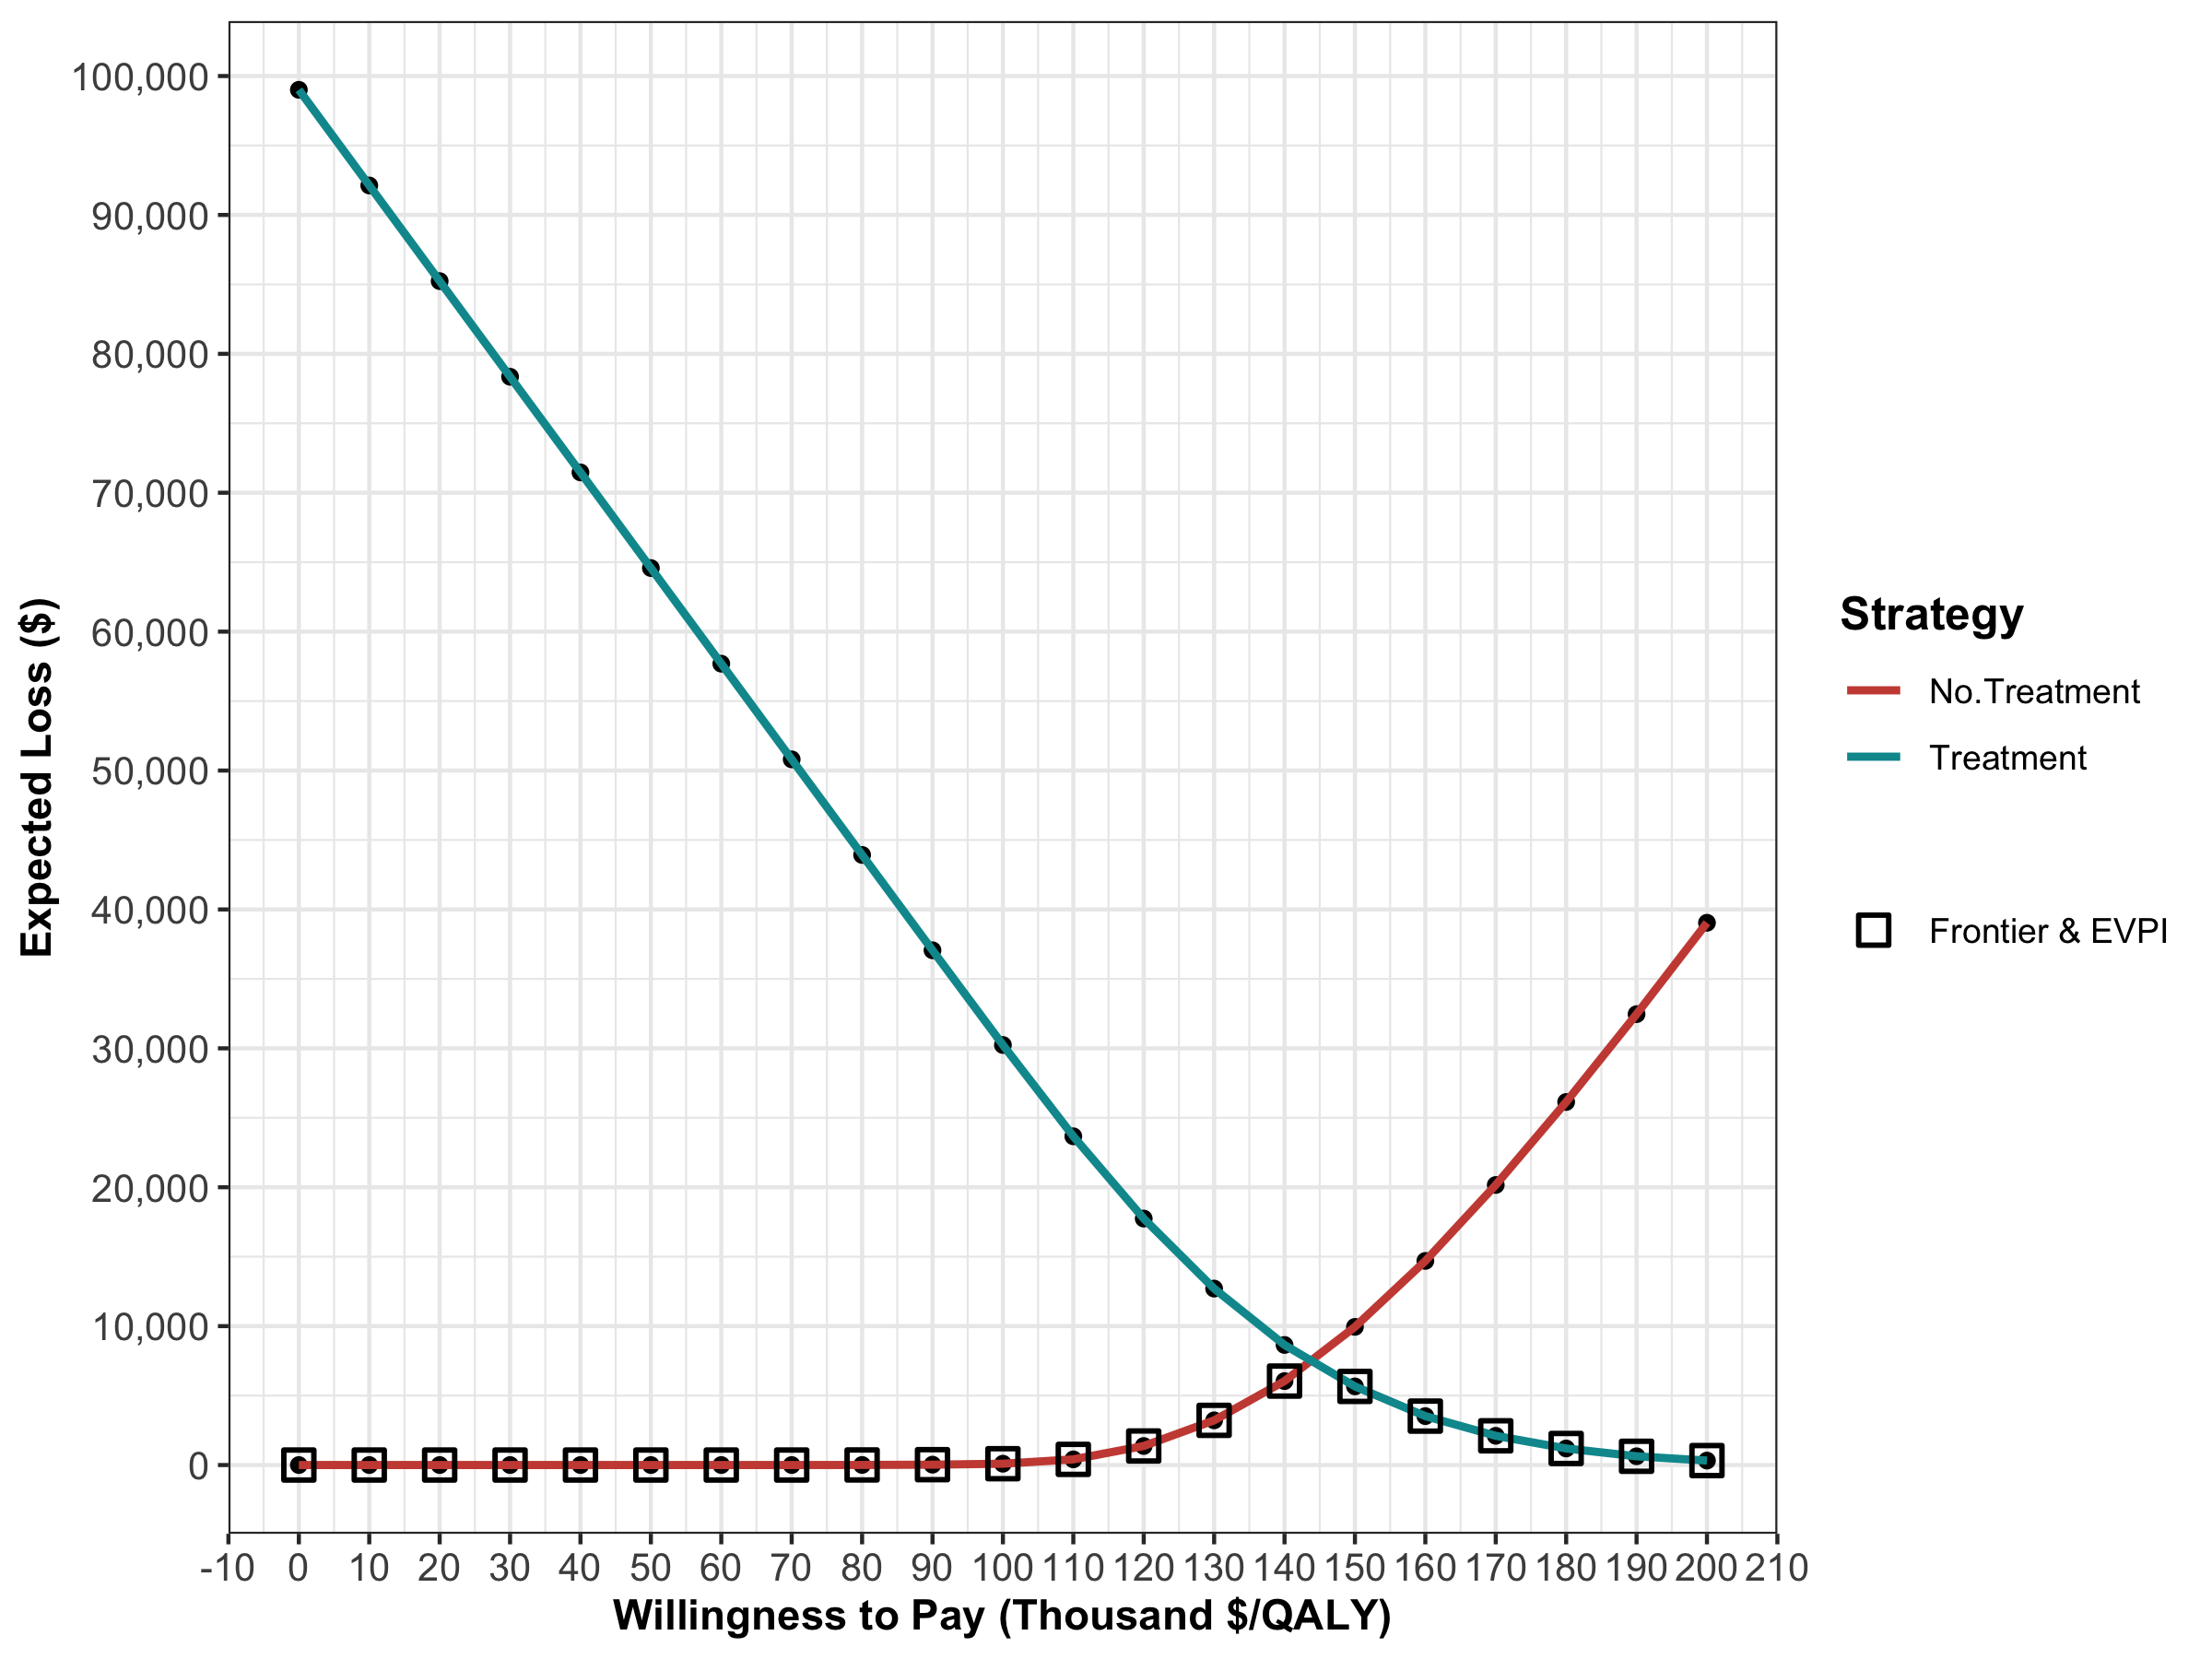
\includegraphics{../figs/05b_elc.png}
\caption{Expected Loss Curves \label{fig:05b_elc}}
\end{figure}

\begin{figure}
\centering
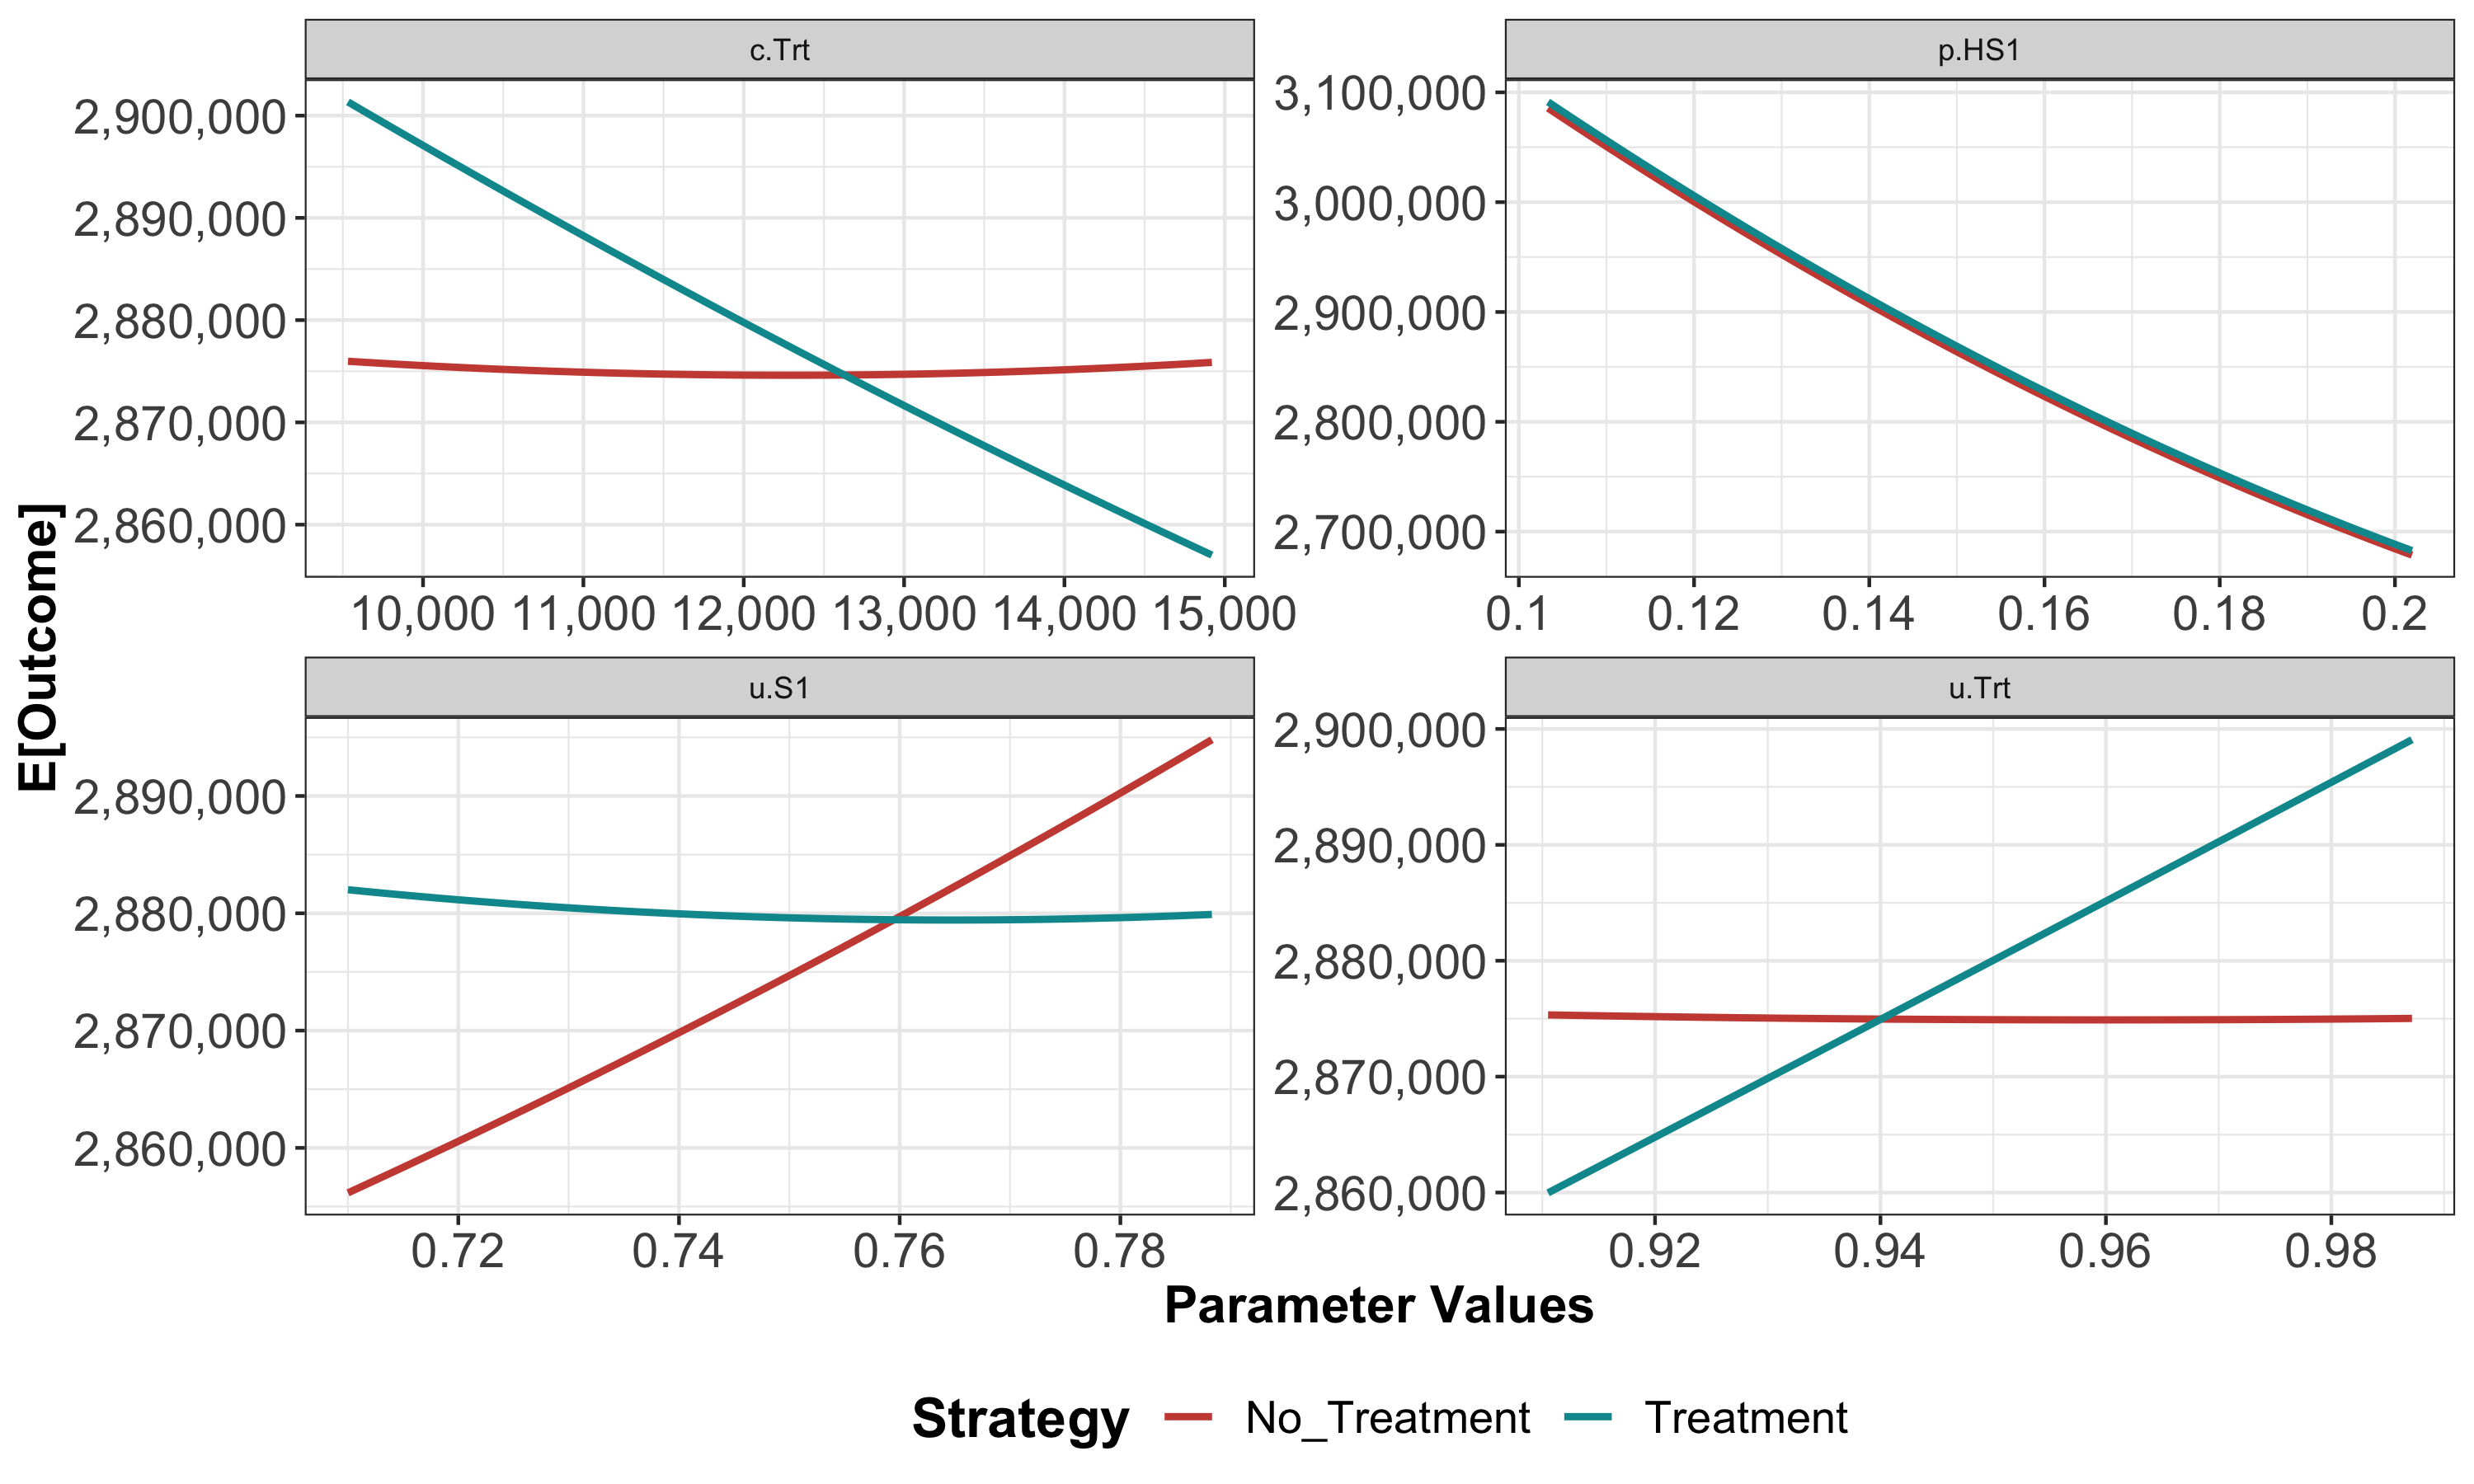
\includegraphics{../figs/05b_owsa-lrm-nmb.png}
\caption{One-way sensitivity analysis (OWSA)
\label{fig:05b_owsa-lrm-nmb}}
\end{figure}

\begin{figure}
\centering
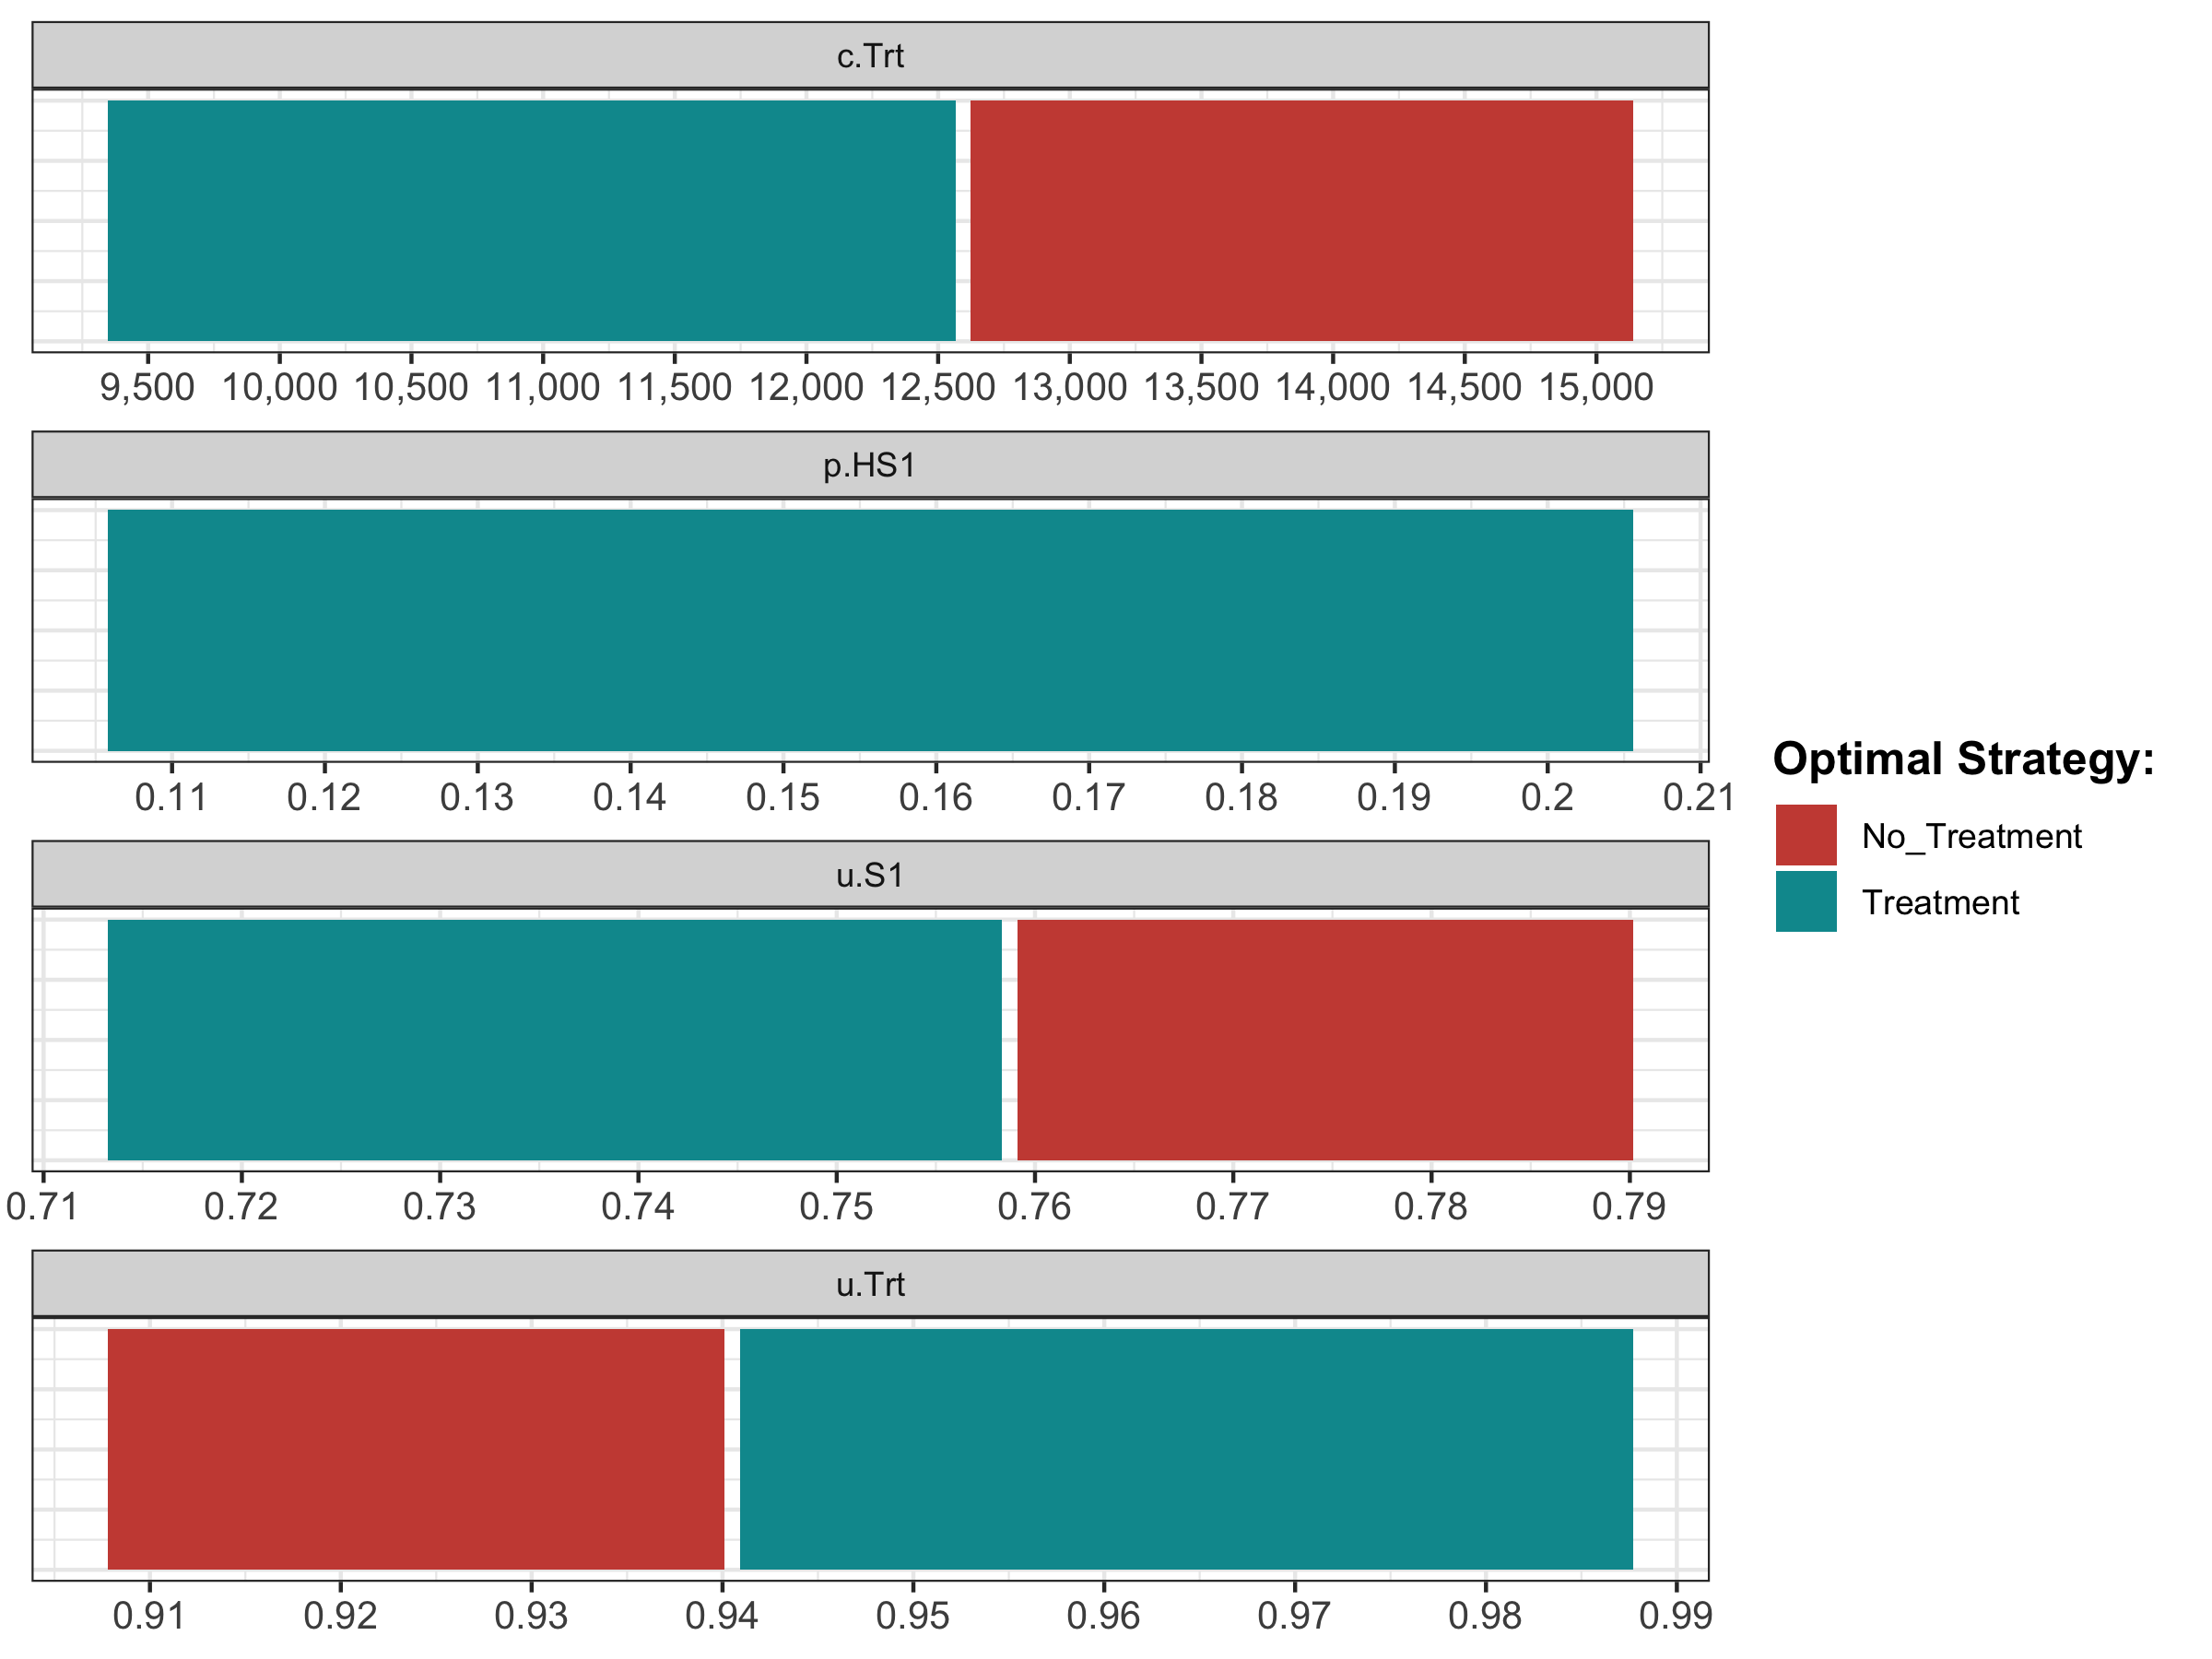
\includegraphics{../figs/05b_optimal-owsa-lrm-nmb.png}
\caption{Optimal strategy with OWSA
\label{fig:05b_optimal-owsa-lrm-nmb}}
\end{figure}

\begin{figure}
\centering
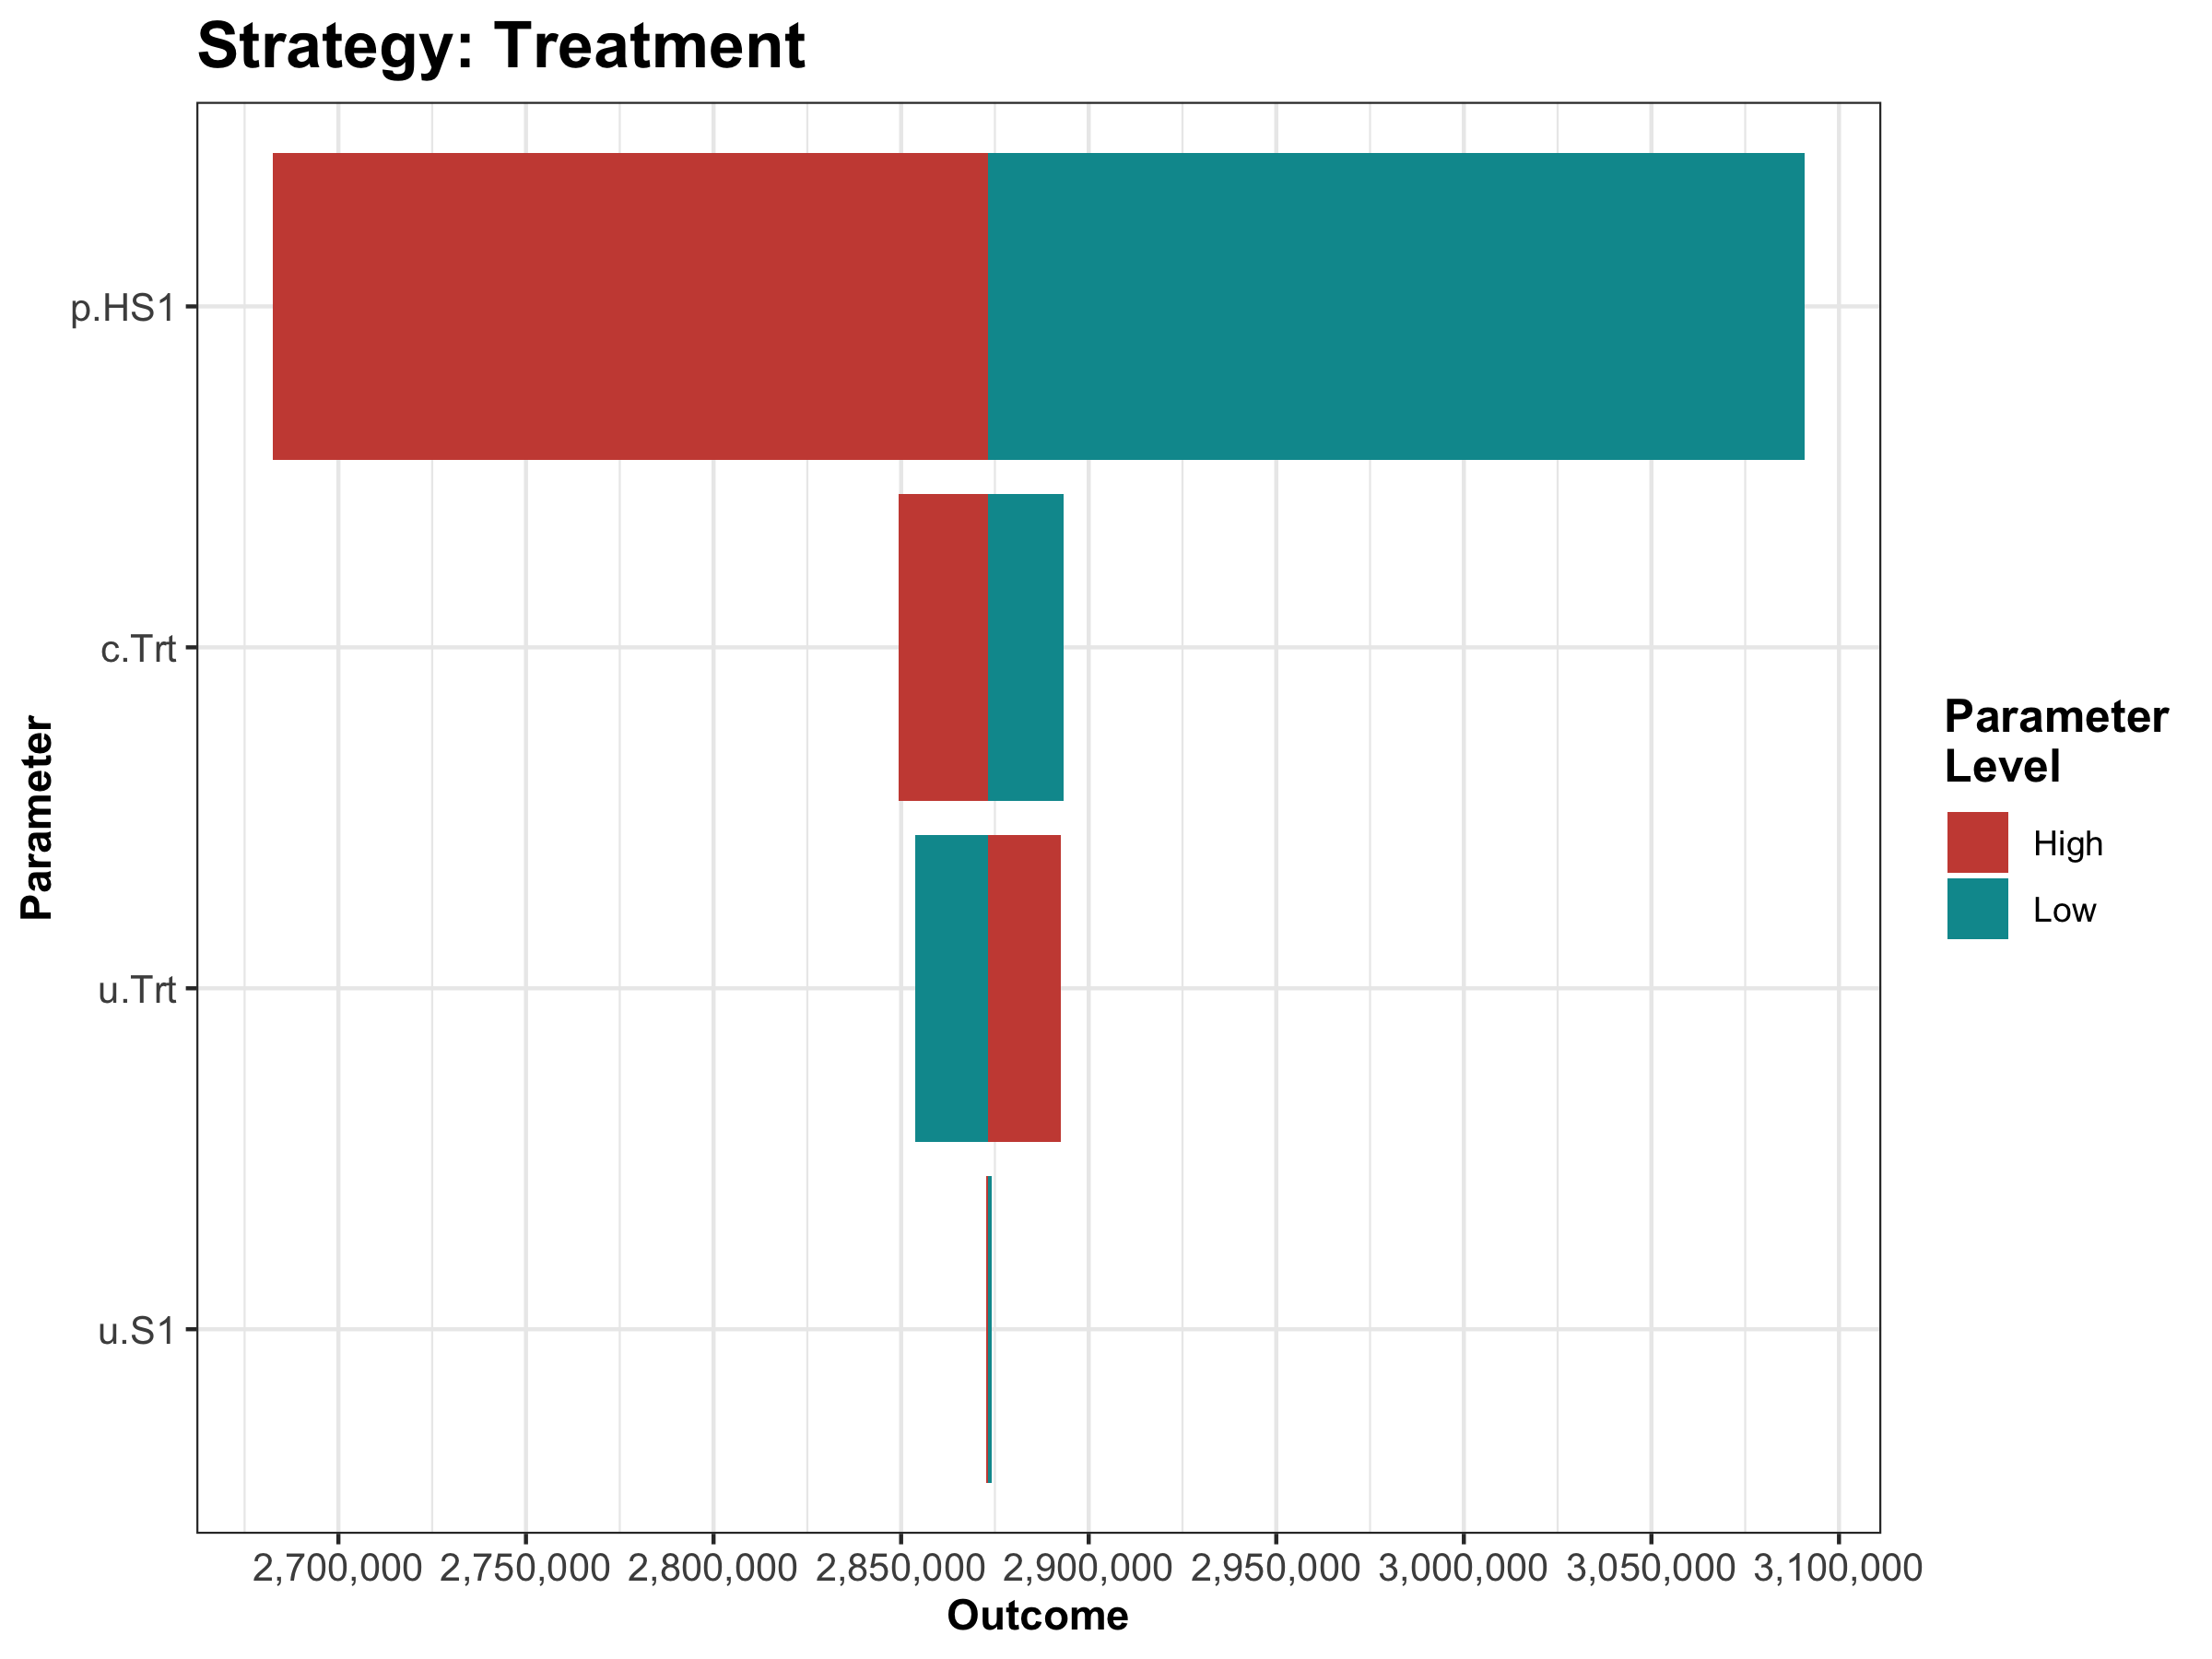
\includegraphics{../figs/05b_tornado-lrm-Treatment-nmb.png}
\caption{Tornado plot \label{fig:05b_tornado-lrm-Treatment-nmb}}
\end{figure}

\begin{figure}
\centering
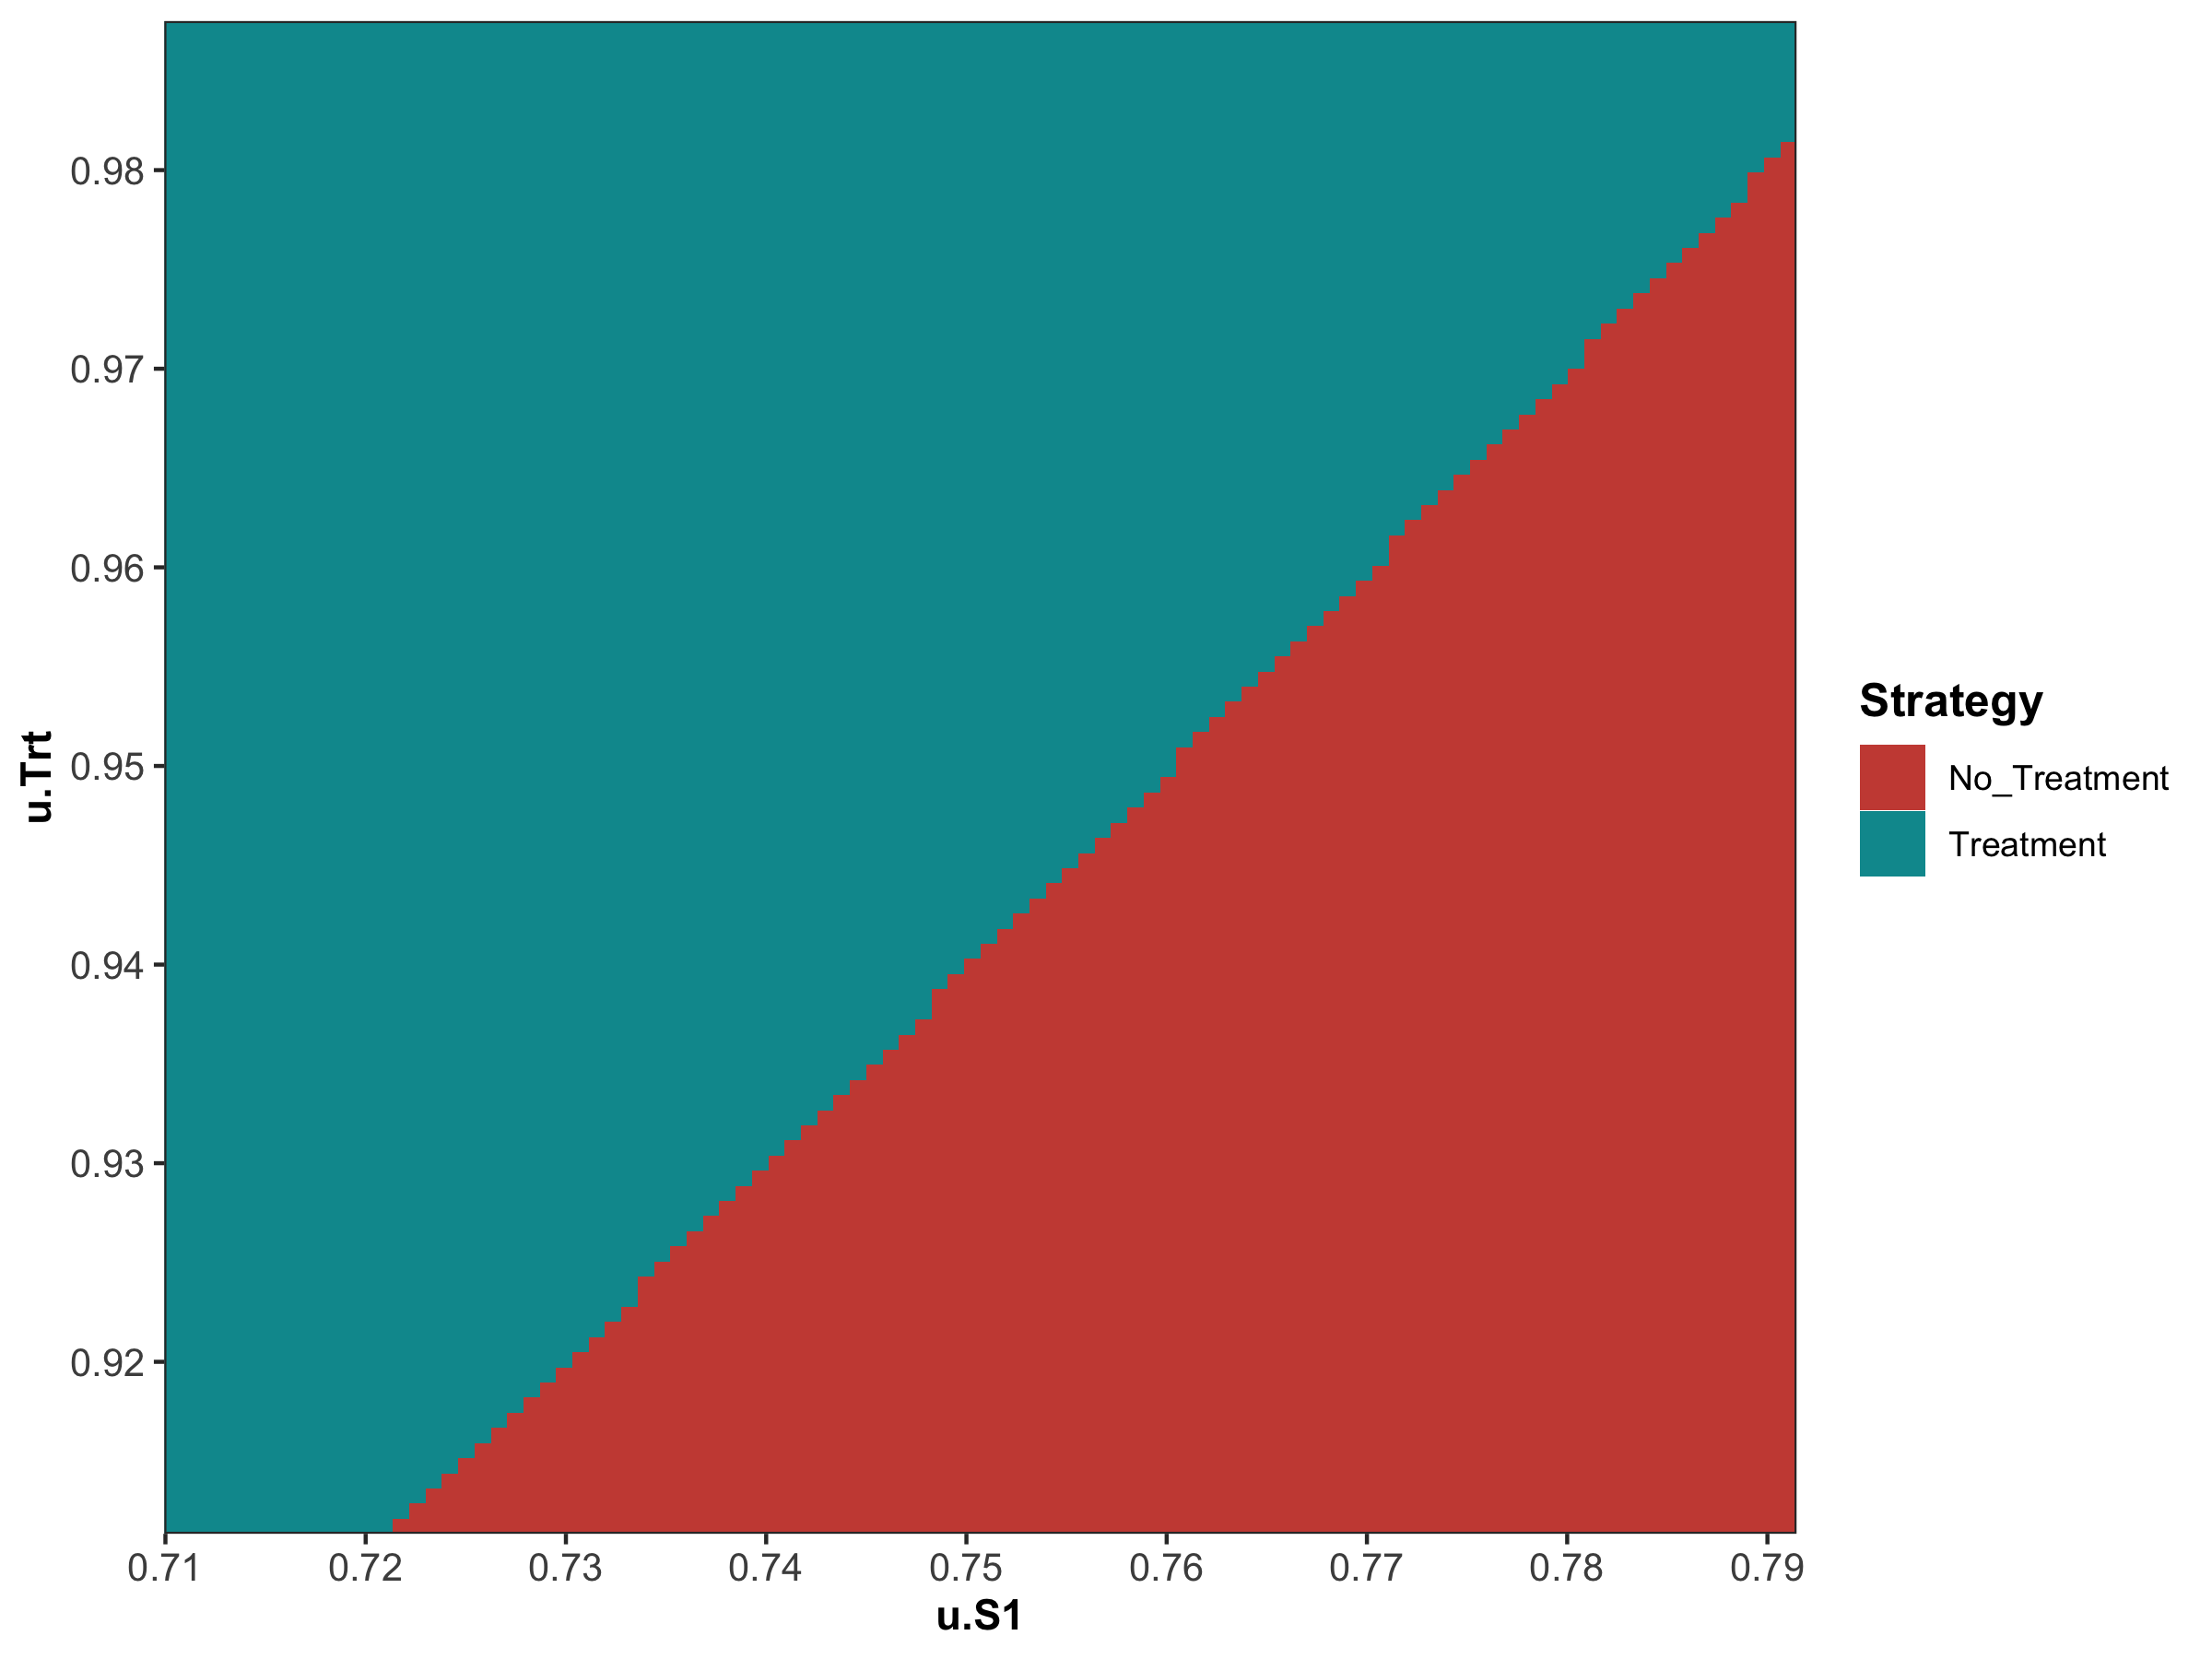
\includegraphics{../figs/05b_twsa-lrm-uS1-uTrt-nmb.png}
\caption{Two-way sensitivity analysis (TWSA)
\label{fig:05b_twsa-lrm-uS1-uTrt-nmb}}
\end{figure}

\paragraph{05c Value of information}\label{c-value-of-information}

In the VOI component, the results from the PSA generated in the
probabilistic analysis subcomponent are used to determine whether
further potential research is needed. We use the \texttt{calc\_evpi}
function from the \texttt{dampack} package to calculate the expected
value of perfect information (EVPI). Figure \ref{fig:05c_evpi} shows the
EVPI for the different WTP values.

\begin{Shaded}
\begin{Highlighting}[]
\NormalTok{evpi <-}\StringTok{ }\KeywordTok{calc_evpi}\NormalTok{(}\DataTypeTok{wtp =}\NormalTok{ v.wtp, }\DataTypeTok{psa =}\NormalTok{ l.psa)}
\end{Highlighting}
\end{Shaded}

\begin{figure}
\centering
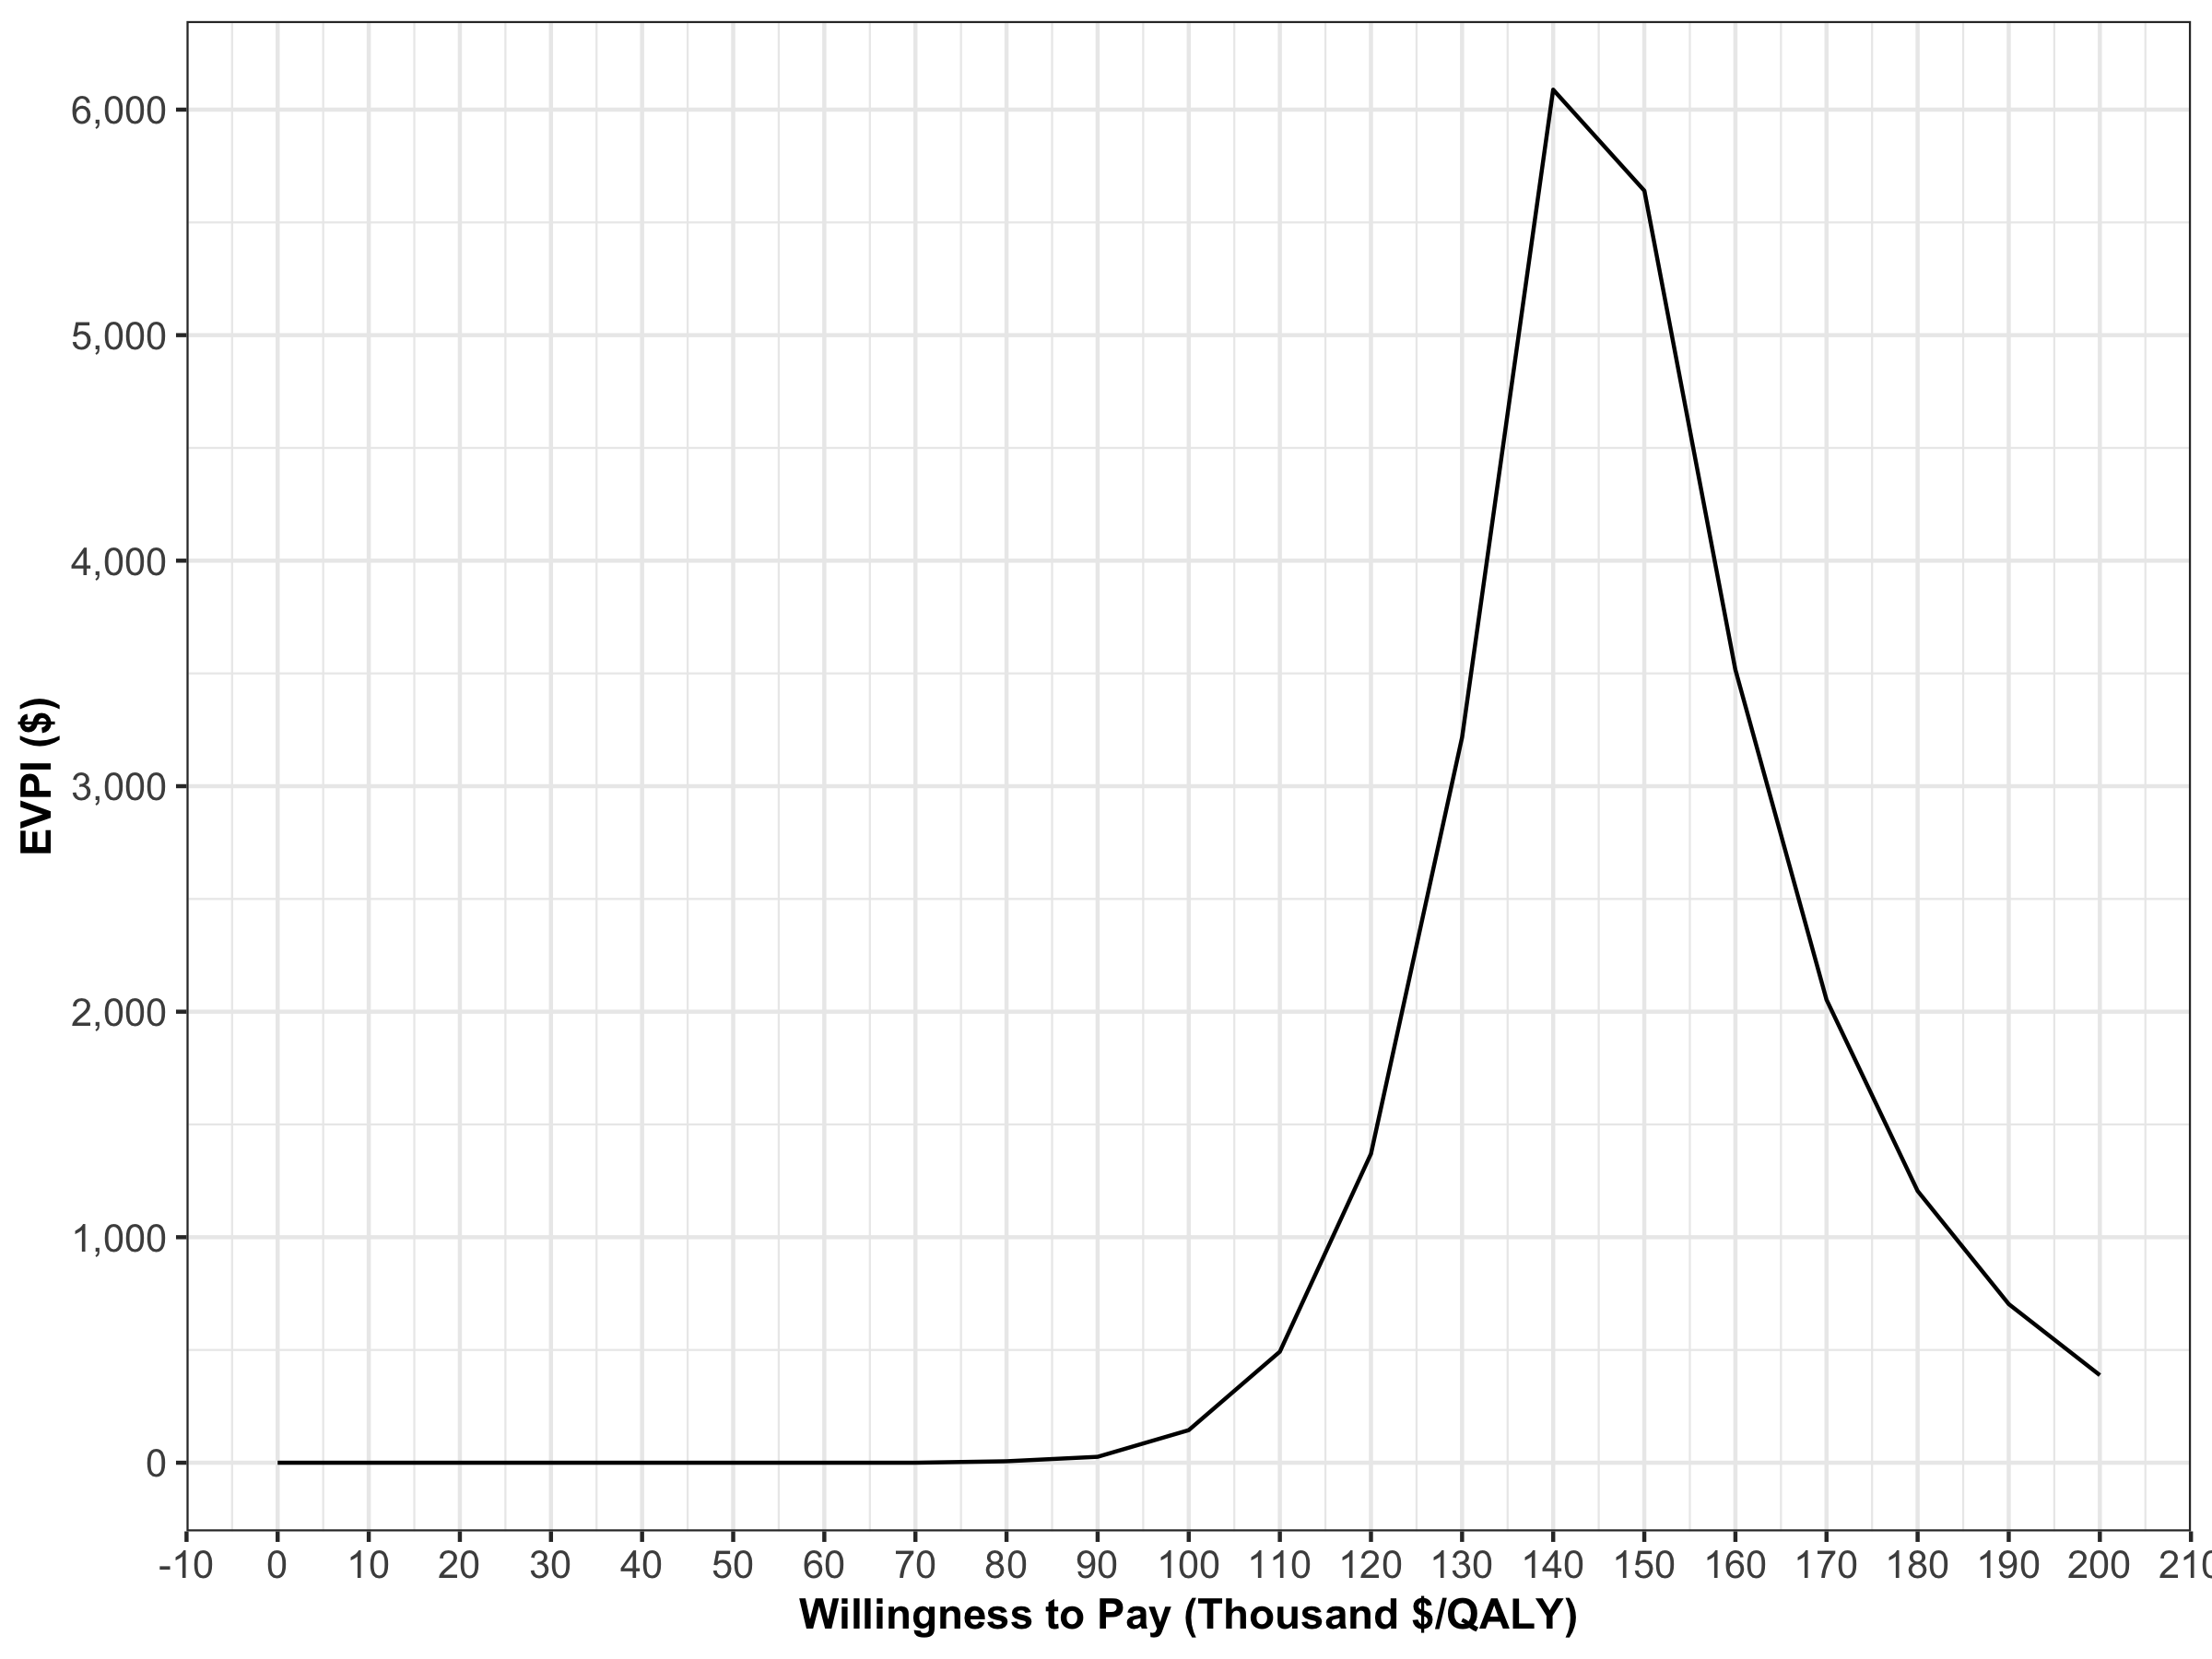
\includegraphics{../figs/05c_evpi.png}
\caption{Expected value of perfect information \label{fig:05c_evpi}}
\end{figure}

\newpage

\subsubsection*{References}\label{references}
\addcontentsline{toc}{subsubsection}{References}

\hypertarget{refs}{}
\hypertarget{ref-Alarid-Escudero2019}{}
Alarid-Escudero, F, EA. Enns, KM. Kuntz, TL. Michaud, and H Jalal. 2019.
```Time Traveling Is Just Too Dangerous' But Some Methods Are Worth
Revisiting: The Advantages of Expected Loss Curves Over
Cost-Effectiveness Acceptability Curves and Frontier.'' \emph{Value in
Health} In Press.

\hypertarget{ref-Alarid-Escudero2018b}{}
Alarid-Escudero, F, RF MacLehose, Y Peralta, KM Kuntz, and Enns EA.
2018. ``Nonidentifiability in Model Calibration and Implications for
Medical Decision Making.'' \emph{Medical Decision Making} 38 (7):
810--21.
doi:\href{https://doi.org/10.1177/0272989X18792283}{10.1177/0272989X18792283}.

\hypertarget{ref-Eddy2012}{}
Eddy, David M., William Hollingworth, J. Jaime Caro, Joel Tsevat,
Kathryn M. McDonald, and John B. Wong. 2012. ``Model transparency and
validation: A report of the ISPOR-SMDM modeling good research practices
task force-7.'' \emph{Medical Decision Making} 32 (5): 733--43.
doi:\href{https://doi.org/10.1177/0272989X12454579}{10.1177/0272989X12454579}.

\hypertarget{ref-Enns2015}{}
Enns, E A, L E Cipriano, C T Simons, and C Y Kong. 2015. ``Identifying
Best-Fitting Inputs in Health-Economic Model Calibration: A Pareto
Frontier Approach.'' \emph{Medical Decision Making} 35 (2): 170--82.
doi:\href{https://doi.org/10.1177/0272989X14528382}{10.1177/0272989X14528382}.

\hypertarget{ref-Goldhaber_Fiebert2010}{}
Goldhaber-Fiebert, JD, NK Stout, and SJ Goldie. 2010. ``Empirically
evaluating decision-analytic models.'' \emph{Value in Health} 13 (5):
667--74.
doi:\href{https://doi.org/10.1111/j.1524-4733.2010.00698.x}{10.1111/j.1524-4733.2010.00698.x}.

\hypertarget{ref-Iskandar2018}{}
Iskandar, R. 2018. ``A theoretical foundation for state-transition
cohort models in health decision analysis.'' \emph{PloS One} 13 (12).
Public Library of Science: e0205543--e0205543.
doi:\href{https://doi.org/10.1371/journal.pone.0205543}{10.1371/journal.pone.0205543}.

\hypertarget{ref-Jalal2013}{}
Jalal, Hawre, Bryan Dowd, François Sainfort, and Karen M. Kuntz. 2013.
``Linear regression metamodeling as a tool to summarize and present
simulation model results.'' \emph{Medical Decision Making} 33 (7):
880--90.
doi:\href{https://doi.org/10.1177/0272989X13492014}{10.1177/0272989X13492014}.

\hypertarget{ref-Menzies2017}{}
Menzies, Nicolas A., Djøra I. Soeteman, Ankur Pandya, and Jane J. Kim.
2017. ``Bayesian Methods for Calibrating Health Policy Models: A
Tutorial.'' \emph{PharmacoEconomics} 35 (6). Springer International
Publishing: 613--24.
doi:\href{https://doi.org/10.1007/s40273-017-0494-4}{10.1007/s40273-017-0494-4}.

\hypertarget{ref-modeest}{}
Poncet, P. 2018. ``Modeest: Mode Estimation.''
\url{https://CRAN.R-project.org/package=modeest}.

\hypertarget{ref-Raftery2010}{}
Raftery, A, and L Bao. 2010. ``Estimating and Projecting Trends in
HIV/AIDS Generalized Epidemics Using Incremental Mixture Importance
Sampling.'' \emph{Biometrics} 66 (4): 1162--73.

\hypertarget{ref-IMIS}{}
Raftery, Adrian, and Le Bao. 2012. \emph{IMIS: Increamental Mixture
Importance Sampling}. \url{https://CRAN.R-project.org/package=IMIS}.

\hypertarget{ref-Rutter2018}{}
Rutter, C, J Ozik, M DeYoreo, and Collier N. 2018. ``Microsimulation
Model Calibration using Incremental Mixture Approximate Bayesian
Computation.'' \emph{arXiv}, no. april: 1--20.
\url{https://arxiv.org/abs/1804.02090v3}.

\hypertarget{ref-Steele2006}{}
Steele, R, A Raftery, and M Emond. 2006. ``Computing Normalizing
Constants for Finite Mixture Models via Incremental Mixture Importance
Sampling (IMIS).'' \emph{Journal ofComputational and Graphical
Statistics} 15 (3): 712--34.
doi:\href{https://doi.org/10.1198/106186006X132358}{10.1198/106186006X132358}.


\end{document}
